\documentclass[10pt,a5paper]{book}
\usepackage{./estilos/paquetes}
\usepackage{./estilos/colores}
\newtheorem{teorema}{Teorema}[chapter]
\usepackage{amsthm}%para definir ecuaciones
\usepackage{amssymb}%para poner dibujos en latex
\usepackage{slashbox}%para poner diagonales en tablas
\usepackage{listings}
\usepackage{multirow}
\usepackage{pdflscape} %para poner horizontal el texto
\usepackage{fancyhdr}%para modificar los encabezados
\usepackage{tocbibind}%para poner bibliografía en el índice
\usepackage[figure,ruled,vlined,linesnumbered,algosection,portugues]{algorithm2e}

\oddsidemargin 0 in
%\textheight 5.7 in
%\textwidth 3.75 in
%\topmargin 0 in
%\parindent 0 em
\let\headwidth\textwidth
\let\footwidht\textwidth


\title{Introducción a la teoría de grafos}
\author{Moisés Gautier Gómez}
\date{}
\setcounter{subsection}{1}
\newtheorem{cor}[]{Corolario}[chapter]
\newtheorem{lem}[]{Lema}[chapter]

\begin{document}
\renewcommand{\tablename}{Tabla}
\renewcommand{\listtablename}{Índice de Tablas}

\frontmatter
\maketitle
\chapter*{}

\emph{Dedicado a mis padres y a mi tutor de proyecto fin de carrera Antonio Tomeu}

\clearpage

\tableofcontents
\listoftables
\listoffigures
\mainmatter
\chapter[Intro. grafos y complej. Algorítmica]{Introducción de grafos y complejidad algorítmica}
La mayoría de los problemas de grafos requieren un recorrido sistemático o búsqueda de grafos. El método actual de recorrido de grafos puede tener características ventajosas estructurales que hacen de este procedimiento una solución eficiente.
\section{Introducción de grafos}

Geométricamente, se define un grafo como un conjunto de puntos (vértices) en el espacio que están interconectados por un conjunto de líneas (aristas).\newline

\begin{figure}[H]
  \centering
  \caption{ }
  \hrulefill{}\\
  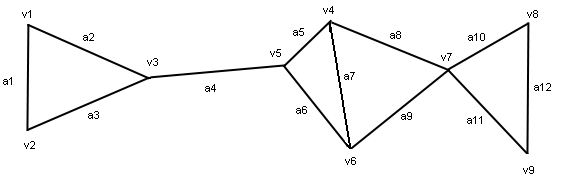
\includegraphics[scale=0.4]{Figura1_1.png}
\end{figure}

\hrulefill{}\\
Para un grafo $G$ denotamos como conjunto de vértices ({$V$}) y como conjunto de aristas ($A$), y escribimos $G = (V, A)$. En la Figura 1.1, tenemos un grafo $G = (\{v_1,v_2, \ldots,v_9\}, \{a_1,a_2, \ldots,a_{12}\})$.

Designaremos al número de vértices en un grafo por $n = |V|$ y el número de aristas por $|E|$. Si tanto $n$ y $|E|$ son finitos, como suele ser generalmente, diremos entonces que el grafo es \textbf{finito}.

Podemos especificar una arista por los dos vértices (llamados puntos finales) que conectan. Si los puntos extremos de $a$ son $v_i$ y $v_j$, entonces podemos escribir $e = (v_i,v_j)$ o $e = (v_j,v_i)$. Así, una definición equivalente del grafo de la Figura1.1 es la siguiente:

\emph{ G = (V,E), V = \{$v_1,v_2, \ldots,v_9$\}} \newline
\begin{center}
  \emph{ E = \{$(v_1,v_2),(v_1,v_3),(v_2,v_3),(v_3,v_5),(v_4,v_5),(v_4,v_6),$}\newline
  \emph{$       (v_4,v_7),(v_5,v_6),(v_6,v_7),(v_7,v_8),(v_7,v_9),(v_8,v_9)\}$}
\end{center}

Si una arista $a$ tiene $v$ como un punto final, entonces podemos decir que esa arista $a$ es incidente con $v$. Asimismo, si $(u,v)\in A$ entonces u se dice que es adyacente a v.

El grado de un vértice $v$, escrito $g(v)$, es el número de aristas incidentes con v. En la Figura 1.1, tenemos $g(v_1) = g(v_2) = g(v_8) = g(v_9) = 2, g(v_3) = g(v_4) = g(v_5) = g(v_6) = 3$ y $g(v_7) = 4$.

\begin{teorema}
  El número de vértices de grado par en un grafo es uniforme. \end{teorema}

\begin{proof}[Demostración:] Si sumamos los grados de todos los vértices de un grafo entonces el resultado debe ser el doble del número de aristas. Esto es porque cada arista contribuye a la suma de cada uno de sus extremos.
  \[ \sum_{i} g(v_{i}) = 2\cdot |A| \]
  El lado derecho de esta ecuación es un número par, tal como define la parte izquierda de los vértices de grado par.\end{proof}

Un bucle es una arista $(u,v)$ tal que $u=v$. Un ejemplo es $a_1$ en el grafo de la Figura 1.2(a). Una arista paralela no puede identificarse exclusivamente especificando sus extremos solamente. En la Figura 1.2(a),$a_2$ es paralelo a $a_3$. En esta sección cuando se trate el concepto de grafos simples, estaremos hablando de grafos que \textbf{no} contienen bucles ni aristas paralelas. Por supuesto, todos los grafos tienen un grafo simple subyacente obtenido por la eliminación del bucle y de las aristas paralelas del grafo inicial. Además para el término multigrafo lo definiremos como un grafo con aristas paralelas pero que no tiene bucles.\newline

\begin{figure}[H]
  \centering
  \caption{ }
  \hrulefill{}\\
  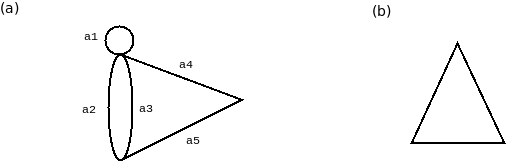
\includegraphics[scale=0.5]{Figura1_2.png}
\end{figure}
\hrulefill{}\newline
Un grafo donde cada par de vértices distintos definen una arista es llamado grafo completo. El grafo completo con $n$ vértices es definido por $K_n$. En un grafo regular (normal) cada vértice tiene el mismo grado, si se corresponde con el valor de $K$ es llamado \emph{k-regular}. Hay que tener en cuenta que $K_n$ es $(n-1)$ regular.\newline

\begin{figure}[H]
  \centering
  \caption{ }
  \hrulefill{}\\
  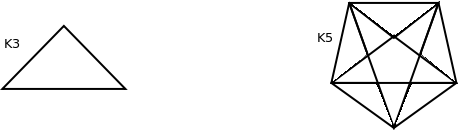
\includegraphics[scale=0.47]{Figura1_3.png}
\end{figure}
\begin{figure}[H]
  \centering
  \caption{ }
  \hrulefill{}\\
  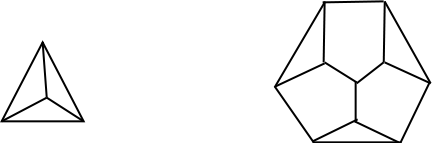
\includegraphics[scale=0.45]{Figura1_4.png}
\end{figure}
\hrulefill{}\\

Si es posible la partición de los vértices de un grafo en dos subconjuntos, $V_{1}$ y $V_{2}$, de manera que cada arista de $G$ una un vértice de $V_{1}$ con un vértice de $V_{2}$, entonces decimos que $G$ puede ser \emph{bipartito}\footnote{bipartito,ta: adj. Que consta de dos partes}. Si cada vértice de $V_1$ esta conectado a cada vértice de $V_2$ entonces se dice que $G$ es un grafo bipartito completo. En este caso se denota al grafo por $K_{i,j}$ donde $|V_1| = i$ y $|V_2| = j$.
\pagebreak
\begin{figure}
  \caption{ }
\hrulefill{}\\
\end{figure}
\begin{flushleft}
  \textbf{(a)}
  \parbox{1cm}
  {
    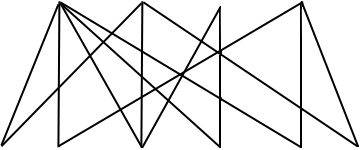
\includegraphics[scale=0.4]{Figura1_5.png}
  }
\end{flushleft}
\begin{flushright}
  \textbf{(b)}
  \parbox{3cm}
  {
    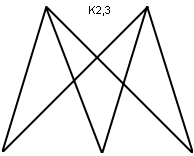
\includegraphics[scale=0.5]{Figura1_5b.png}
  }
\end{flushright}
\hrulefill{}\\

Dos grafos son \emph{isomórficos}\footnote{isomorfismo: Correspondencia biunívoca entre dos estructuras algebraicas que conserva las operaciones.} si hay una correspondencia uno-a-uno entre los vértices de $G_1$ y $G_2$ de tal manera que el número de aristas que une los dos vértices en $G_1$ sea igual al número de aristas que une los dos correspondientes vértices en $G_2$.\\

\begin{figure}[H]
  \centering
  \caption{ }
  \hrulefill{}\\
  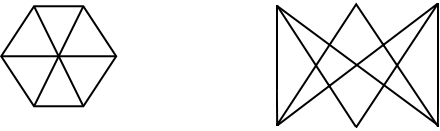
\includegraphics[scale=0.5]{Figura1_6.png}
\end{figure}
\hrulefill{}

Un buen \emph{subgrafo} de $G$ es un grafo obtenido de la eliminación de una serie de aristas y/o vértices de $G$. Si eliminamos una arista $a$ o un vértice $v$ de $G$, los grafos resultantes serán respectivamente denotados como $(G-a)$ y $(G-v)$. Si $H$ es un subgrafo de $G$, entonces $G$ lo podemos llamar como supergrafo de $H$ y lo representamos como $H \subseteq G$. Un subgrafo de $G$ \emph{inducido} por un subconjunto de sus vértices, $V^{'} \subset V$, es el grafo consistente de $V^{'}$ y de aristas de $G$ con ambos extremos en $V^{'}$

Un \emph{camino} desde $v_1$ hasta $v_i$ es una secuencia $P = v_1,a_1,v_2,\\a_2, \ldots,a_{i-1},v_i$ de vértices alternos y aristas de forma que $1 \le j < i, a_j$ es incidente con $v_j$ y $v_{j+1}$. Si $v_1 = v_i$ entonces $P$ se dice que es un \emph{ciclo} o un \emph{circuito}. En un grafo simple un camino o un ciclo $v_1,a_1,v_2,a_2, \ldots,a_{i-1}$ puede ser especificado de una forma más simple por la secuencia de vértices $v_1,v_2, \ldots,v_i$. Si un camino desde cada vértice sólo aparece una vez, entonces la secuencia se llama \emph{camino sencillo}. Si cada vértice aparece una vez, excepto cuando $v_1 = v_i$ entonces $P$ es un circuito \emph{simple}. La \emph{longitud} de un camino o un ciclo es el número de aristas que contiene. Dos caminos son \emph{disjuntos} si no tienen alguna arista en común.

Dos vértices $v_i$ y $v_j$ están conectados si existe un camino desde $v_i$ hasta $v_j$. Los subgrafos inducidos a su vez por los subconjuntos $V_1,V_2, \ldots,V_k$, se llaman \emph{componentes} del grafo. Un grafo conexo solo tiene una componente, de lo contrario no es conexo. Así, el grafo de la Figura1.1 es conexo mientras que el de la Figura1.9 tiene dos componentes.

Un subgrafo de \emph{expansión} de un grafo conexo $G$ es un subgrafo de $G$ que se obtiene eliminando aristas únicamente y de forma que cualquier par de vértices siguen permaneciendo conectados. Si la supresión de un vértice $v$ desconecta $H$, entonces $v$ se puede decir que es un \emph{punto de articulación}.

Un grafo con uno o más puntos de articulación se llama también un grafo \emph{separable}.

En algunas aplicaciones, es natural asignar una \emph{dirección} a cada arista del grafo. Así, en un diagrama de un grafo cada arista es representada por una flecha. Un grafo representado de esta manera se llama grafo \emph{dirigido} o \emph{dígrafo}.\\

\begin{figure}[H]
  \centering
  \caption{ }
\hrulefill{}\\
  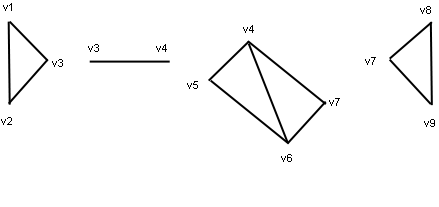
\includegraphics[scale=0.5]{Figura1_7.png}
\end{figure}
\begin{figure}[H]
  \centering
  \caption{ }
  \hrulefill{}\\
  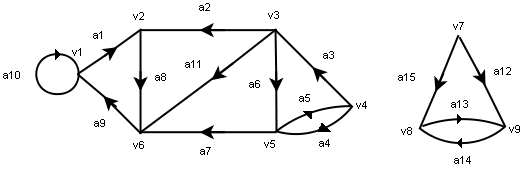
\includegraphics[scale=0.5]{Figura1_8.png}
\end{figure}
\hrulefill{}\\

Para el vértice $v$, la salida $g^{+}(v)$ y la entrada $g^{-}(v)$ son, incidentes respectivamente, el número de aristas incidentes desde $v$ y el número de aristas incidentes hacia $v$. Un dígrafo \emph{simétrico} es un dígrafo en el que por cada arista $(v_i,v_j)$ hay otra arista $(v_j,v_i)$. Un dígrafo es \emph{equilibrado} si para cada vértice $v$, $g^{+}(v) = g^{-}(v)$.

Todo dígrafo tiene un \emph{grafo subyacente} (\emph{no dirigido y simple}) que se obtiene mediante la supresión de las direcciones de las aristas. Así, la Figura1.9 muestra este grafo para el
 subgrafo de la Figura1.8. Según la definición anterior, un camino (o circuito) en un grafo no dirigido corresponde a una secuencia $S = v_1,a_1,v_2,a_2, \ldots,v_{i-1},a_i$ de vértices y aristas. En el dígrafo asociado a esta secuencia puede ser tal que\\

\begin{figure}[H]
  \centering
  \caption{ }
  \hrulefill{}\\
  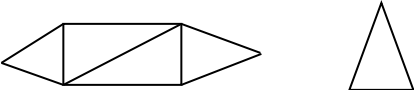
\includegraphics[scale=0.5]{Figura1_9.png}
\end{figure}
\hrulefill{}\\

para todos los $j, 1 \le j < i, a_j$ es incidente desde $v_j$ e incidente hacia $v_{j+1}$. En este caso $S$ se dice que es un camino (o circuito) \emph{dirigido}. De lo contrario sería un camino (o circuito) \emph{no dirigido}. Así en la Figura1.8 $(v_2,a_2,v_3,a_6,v_5,a_4,v_4,a_3,v_3,a_{11},v_6)$ es un camino simple no dirigido, mientras que $(v_1,a_1,v_2,a_8,v_6,\\a_9,v_1)$ es un circuito simple dirigido. Porque en un dígrafo podemos definir dos tipos diferentes de conexión. Dos vértices, $v_1$ y $v_2$, se dice que están \emph{fuertemente conectados} si existe un camino dirigido desde $v_1$ a $v_2$ y un camino dirigido desde $v_2$ a $v_1$. Si $v_1$ y $v_2$ no están fuertemente conectados, pero están conectados en el grafo no dirigido correspondiente, entonces $v_1$ y $v_2$ se dice que están \emph{débilmente conectados}.

Tanto la fuerte conexión como la débil conexión son relaciones de equivalencia\footnote{Sea $K \notin \emptyset$ y $R$ una relación binaria definida sobre $K$. Se dice que R es una relación de equivalencia si cumple que:\begin{itemize}
\item Es reflexiva. 
\item Es simétrica. 
\item Es transitiva.\end{itemize}} en el conjunto de vértices de un dígrafo.

Así, para el grafo de la Figura1.8, las particiones de conexión débil en los vértices de los dos subconjuntos $\{v_1,v_2,v_3,v_4,v_5,v_6\}$ y $\{v_7,v_8,v_9\}$. Los subgrafos inducidos por estos subgrupos se llaman \emph{componentes débilmente conexos} del dígrafo. Por otro lado tenemos una partición fuertemente conexa de los vértices del grafo para los subconjuntos $\{v_1,v_2,v_6\},\{v_3,v_4,v_5\},\{v_7\}$ y $\{v_8,v_9\}$. Cada uno de estos subconjuntos induce una \emph{componente fuertemente conexa} del dígrafo.

Un \emph{bosque} es un grafo cuyas componentes son árboles. Un \emph{árbol externo} es un árbol dirigido en donde, precisamente, uno de los vértices tiene cero grados internos. Del mismo modo, un árbol interno es un árbol dirigido en el que precisamente tiene cero grados externos. Un árbol en el que un vértice, la raíz, es distinguible, es llamado \emph{árbol raíz}. En un árbol cualquier vértice de grado uno, a menos que sea la raíz, se llama \emph{hoja}. La \emph{profundidad} o \emph{nivel} de un vértice en un árbol es el número de aristas en el camino desde la raíz hasta dicho vértice. Si $(u,v)$ es una arista de un árbol de tal manera que $u$ está en el camino desde la raíz a $v$, entonces $u$ se dice que es el \emph{padre} de $v$ y $v$ es el \emph{hijo} de $u$. Un \emph{antepasado} (o \emph{ancestro}) de $u$ es cualquier vértice del camino desde $u$ hasta la raíz del árbol. Un antepasado \emph{adecuado} de $u$ es cualquier antepasado de $u$ excluyendosé al propio $u$. De manera similar, si $u$ es un antepasado de $v$, entonces $v$ es un \emph{descendiente} de $u$. Por último, un \emph{árbol binario} es un árbol en el que cada vértice, a menos que sea una hoja, tiene dos hijos.

\begin{teorema}
\label{teorema1.2}
  Si $T$ es un árbol con n vértices, entonces:
  \begin{description}
  \item[(a)] Cualquier par de vértices de $T$ están conectados precisamente por un camino.
  \item[(b)] Para cualquier arista a, que no este en $T$, pero que conecte dos vértices de $T$, el grafo $(T+a)$ contiene exactamente un camino.
  \item[(c)] $T$ tiene $(n-1)$ aristas.
  \end{description}
\end{teorema}
\begin{proof}
  \textbf{(a)} $T$ está conectado y por lo menos existe al menos un camino entre dos vértices $u$ y $v$. Supongamos que dos caminos distintos $P_1$ y $P_2$ existen entre $u$ y $v$. Siguiendo estos caminos desde $u$ hasta $v$, dejamos que el primero diverga\footnote{Divergir: Dicho de dos o más líneas o superficies: Irse apartando sucesivamente unas de otras.} hacia $u$ y el segundo converga\footnote{Convergir: Dicho de dos o más líneas: Dirigirse a unirse en un punto.}hacia $v$. La sección de $P_1$ desde $u^{'}$ hasta $v^{'}$ seguida por la sección de $P_2$ desde $v^{'}$ hasta $u^{'}$ debería formar un circuito. Por definición, T no contiene circuitos y por lo tanto llegamos a una contradicción.\\
  \textbf{(b)} Sea $a = (u,v)$. De acuerdo con \textbf{(a)} no es precisamente un camino $P$ desde $u$ hasta $v$ en $T$. La adición de a por tanto crea un circuito $(P+a)$.\\
  \textbf{(c)} La prueba es por inducción sobre el número de vértices $n$ en $T$. Si $n=1$ o $2$, entonces, trivialmente, el número de aristas de T es $(n-1)$. Suponemos que el enunciado es verdadero para todos los árboles con menos de $n$ vértices. Sea $T$ con $n$ vértices. Tiene que haber un vértice de un grado que figura en $T$, de lo contrario podríamos realizar un circuito siguiendo cualquier camino desde vértice a vértice entrando por el extremo de un vértice y saliendo por el otro.
\end{proof}

Completamos nuestro catálogo de definiciones mediante la introducción de grafos \emph{ponderados}. En algunas aplicaciones es natural asignar un número a cada arista del grafo. Para cualquier arista a, este número lo escribiremos como $w(a)$ y se llamará peso. Naturalmente, el grafo en cuestión se llama \emph{grafo ponderado}. El peso de un \emph{(sub)grafo} es igual a la suma de los pesos de sus aristas. A menudo cuando nos refiramos al término camino (o ciclo) podría resultar más apropiado referirse a la longitud más que el peso del camino (o ciclo).

\section[Intro. complejidad algorítmica]{Introducción a la complejidad algorítmica}

Nuestro interés en la eficiencia está particularmente centrado en lo que se denomina el \emph{tiempo de la complejidad de los algoritmos}. Dado que el concepto análogo de \emph{complejidad-espacio} será de poco interés para nosotros, podemos usar el término \emph{complejidad} de una manera inequívoca. La\emph{complejidad} de un algoritmo es simplemente el número de pasos computacionales que se requieren para transformar los datos de entrada en un resultado de un cálculo. En general, esta es una función sobre la cantidad de datos de entrada, comúnmente llamado \emph{tamaño del problema}. Para algoritmos de grafos el tamaño del problema es determinado por uno o quizás dos de las variables $n$ y $|A|$.

Para un tamaño de problema $s$, se denota a la complejidad de un algoritmo de grafo $AL$ por $C_{AL}(s)$, dejando caer el subíndice $AL$ cuando no surga ambigüedad. $C_{AL}(s)$ puede variar significativamente si el algoritmo $AL$ se aplica a grafos estructuralmente diferentes pero que sin embargo son del mismo tamaño. En este texto se toma $C_{AL}(s)$ en el sentido de la complejidad del peor caso. A saber, el número máximo, de todos los tamaños de entrada computacional de $s$, necesarios para la ejecución del algoritmo.

La complejidad de dos algoritmos para el mismo problema, en general son diferentes. Sea $AL_1$ y $AL_2$ dos algoritmos y supongamos que $C_{AL_{1}}(n) = \frac{1}{2}n^2$ y que $C_{AL_{2}}(n) = 5n$. Luego $AL_2$ es más rápido que $AL_1$ para todos los tamaños del problema $n>10$. De hecho lo que habían sido los (finito y positivo) coeficientes de $n^2$ y de $n$ en estas expresiones, $AL_2$ sería más rápido que $AL_1$ para todo $n$ mayor que cierto valor $n_0$ dado. La razón, por supuesto, es que el crecimiento asintótico, como el tamaño del problema tiende a infinito, de $n^2$ es mayor que el de $n$. La complejidad de $AL_2$ se dice que es de orden menor que el de $AL_1$. La idea del orden de una función es importante en la teoría de la complejidad y ahora tenemos que definir y aún más ilustrar.

Dadas dos funciones $F$ y $G$, cuyo dominio son los números naturales, decimos que el orden de $F$ es inferior o igual al orden de $G$ provando que: \[ F(n) \le  K\cdot G(n) \]
para todo $n > n_0$, donde $K$ y $n_0$ son dos constantes positivas. Si el orden de $F$ es inferior o igual al orden de $G$, entonces podemos escribir $F = O(G)$ o decimos que $F$ es $O(G)$. $F$ y $G$ son del mismo orden previsto así que $F = O(G)$ y tal que $G = O(F)$. A veces es conveniente escribir $\Theta(G)$ para especificar el conjunto de todas las funciones que son del mismo orden que $G$. Aunque $\Theta(G)$ se define como un conjunto, que convencionalmente escribiriamos como $F = \Theta(G)$ en el sentido de $F \in \Theta(G)$. Para ilustrar estas definiciones, vemos que $5n$ es $O(\frac{1}{2}n^2)$ pero $5n \ne \Theta(\frac{1}{2}n^2)$ porque $\frac{1}{2}n^2$ no es $O(5n)$. Así el polinomio $(3n^3 + 6n^2 + n + 6)$ es $O(n^3)$.

Cuando se comparan dos funciones en términos de orden, a menudo es conveniente tomar la siguiente definición alternativa. Sea \[\lim_{n\rightarrow\infty}\frac{F(n)}{G(n)} = L \] vemos que:
\begin{description}
  \item[\textbf{(i)}] Si $L = c$ una constante finita y positiva, entonces $F = \Theta(G)$.
  \item[\textbf{(ii)}] Si $L = 0$, entonces $F$ es de un orden inferior a $G$.
  \item[\textbf{(iii)}] Si $L = \infty$, entonces $G$ es de orden menor que $F$.
\end{description}
Probaremos los siguientes casos:
\begin{description}
  \item[\textbf{(a)}] $F(n) = 3n^2 - 4n + 2$ y $G(n) = \frac{1}{2}n^2$. Por lo tanto $L = 6$, así que $F = \Theta(G)$.
  \item[\textbf{(b)}] $F(n) = \log_2 n$ y $G(n) = n$. Entonces:\[ L = \lim_{n\rightarrow\infty}\frac{\ln n}{n}\cdot\log_{2}e = \lim_{n\rightarrow\infty}\bigg(\frac{\log_{2}e}{n}\bigg)=0\] Aquí hemos utilizado la regla de L'Hôpital que establece que si \[ \lim_{n\rightarrow\infty} F(n) = \lim_{n\rightarrow\infty} G(n) = \infty \] y con tal que las derivadas de $F^{'}$ y $G^{'}$ y los límites existan, tendremos que:\[ \lim_{n\rightarrow\infty}\frac{F(n)}{G(n)} = \lim_{n\rightarrow\infty}\frac{F^{'}(n)}{G^{'}(n)} \]Como $L = 0$, vemos que $\log_2n$ es de orden menor que $n$.
  \item[\textbf{(c)}] $F(n) = x^n$ y $G(n) = n^k$, donde $x$ y $k$ son constantes arbitrarias fijas, ambas mayores que 1. Se define $U(n) = \frac{F(n)}{G(n)}$, de modo que: \[ \frac{U(n+1)}{U(n)} = x\bigg(\frac{n}{(n+1)^k}\bigg) \] Así para un $k$ fijo, siempre podemos encontrar un valor lo suficientemente grande de $n$, $n_0$ sabiendo que para $n > n_0$: \[U(n+1) \simeq x\cdot U(n) \] Por tanto, para $n \ge n_0$ \[ U(n) \simeq x^{n-n_{0}}U(n_0) \] y \[ L = \lim_{n\rightarrow\infty} U(n) = \infty \] De modo que $F$, que es exponencial en $n$, es de orden superior a \emph{cualquier} polinomio en $n$.
\end{description}
El orden de $C_{AL}(s)$ describe el comportamiento asintótico de $C_{AL}(s)$ como $s \rightarrow\infty$. Si $C_{AL}(s)$ es $O(f)$, a continuación podemos decir que $AL$ es de orden $O(f)$. La \emph{complejidad asintótica} determina el mayor tamaño posible para el problema tratado. Si dos algoritmos para el mismo problema son del mismo orden, podemos decir, en términos generales, que no existen mejoras significativas de uno al otro.

En la Tabla 1.1 se han contabilizado diversas complejidades que ocurren comúnmente para una gama de tamaños de problema.
\begin{table}[!hbt]
\begin{center}
\caption{Tiempos de cómputo para una variedad de complejidad-tiempo, en un rango de tamaños de problemas.}
\begin{tabular}{|p{5cm}|l|c|c|c|c}
\hline
\hline
\backslashbox{Complejidad\\tiempo}{Tamaño del\\problema $n$} & 2 & 8 & 128 & 1024 \\
\hline
$n$ & 2 & $2^3$ & $2^7$ & $2^{10}$ \\
\hline
$n \log_2n$ & 2 & $3$x$2^3$ & $7$x$2^7$ & $10$x$2^{10}$ \\
\hline
$n^2$ & $2^2$ & $2^6$ & $2^{14}$ & $2^{20}$ \\
\hline
$n^3$ & $2^3$ & $2^9$ & $2^{21}$ & $2^{30}$ \\
\hline
$2^n$ & $2^2$ & $2^8$ & $2^{128}$ & $2^{1024}$ \\
\hline
$~n!$ & $2$ & $5$x$2^{13}$ & $5$x$2^{714}$ & $7$x$2^{8766}$ \\
\hline
\hline
\end{tabular}
\end{center}
\end{table}
\begin{subequations}
\begin{align}
2^{10} pasos/segundos & \simeq 0.9 x 2^{16} pasos/minuto\nonumber \\ & \simeq 0.9 x 2^{22} pasos/hora\nonumber \\ & \simeq 1.3 x 2^{26} pasos/d\acute{\dotlessi}a\nonumber \\ & \simeq 0.9 x 2^{35} pasos/a\tilde{n}o\nonumber \\ & \simeq 0.7 x 2^{42} pasos/siglo\nonumber
\end{align}
\end{subequations}

La complejidad de un algoritmo es importante para un científico informático. Una razón de esto es que la existencia de un algoritmo no garantiza en la práctica que el problema pueda ser resuelto. El algoritmo puede ser tan ineficiente que, incluso con velocidade de cómputo mucho mayores sobre las que hay actualmente, no sería posible obtener un resultado dentro de un período de tiempo útil. Es necesario entonces para caracterizar los algoritmos que sean suficientemente eficaces para hacer que su aplicación útil y puedan así distinguirse de los que puedan tenerse en cuenta a efectos prácticos.

La distinción técnica, ya que se ha elaborado, entre algoritmos eficientes e ineficientes puede ser vulgar, ya que no tiene en cuenta los coeficientes o el grado de un polinomio en cuestión. Para tamaños de problemas muy pequeños, se puede ver en la Tabla 1 que el algoritmo con complejidad $2^n$ o $n!$ son en realidad más eficientes que el de complejidad $3^n$.

Sin embargo, es cierto que, en la práctica, estas consideraciones son poco frecuentes porque los problemas en tiempo polinómico tratados son de bajo grado, y contienen coeficientes simples. Otro rasgo diferente, es que también debemos recordar que la complejidad de un algoritmo se mide para el comportamiento en el peor caso. Un ejemplo bien conocido, que sale fuera de nuestra definición técnica de la eficiencia, es el del problema de la \emph{programación lineal}.

Se podría pensar que nuestra especificación de la eficiencia, pierde su utilidad con las nuevas generaciones de ordenadores debido que estos últimos funcionan a velocidades más altas. Esto podría ser remarcable pero no es el caso. La mejor manera de ver esto es contabilizar los tamaños máximos de los problemas que pueden resolverse con varias complejidades, durante un período de tiempo común, debido a que la velocidad de cálculo es mayor.

Queda claro, que esto sólo sirve para mejorar nuestra noción de que los algoritmos puedan ser considerados como eficientes.

A pesar de nuestras premisas anteriores, podemos llamar a un problema cuyo tiempo polinómico no sea conocido, y para el que se conjetura que no existe tal algoritmo, un problema \emph{intratable}.
\begin{center}
\begin{table}
  \caption{El efecto de una mayor velocidad en el tamaño de un problema dado que puede resolverse por cualquier polinómio y en un tiempo algorítmico exponencial}
    \begin{tabular}{p{1.9cm}l c c c c}
      \hline
      \hline
      Complejidad & Velocidad & $2^3$ & $2^7$ & $2^{10}$ \\
      & actual & x velocidad & x velocidad & x velocidad \\
      \hline
      $n$ & $N_1$ & $8N_1$ & $128N_1$ & $1024N_1$ \\
      $n^2$ & $N_2$ & $2.8N_2$ & $11.3N_2$ & $32N_2$ \\
      $2^n$ & $N_3$ & $N_3 + 3$ & $N_3 + 7$ & $N_3 + 10$ \\
      $8^n$ & $N_4$ & $N_4 + 1$ & $N_4 + 2.3$ & $N_4 + 3.3$ \\
      \hline
      \hline
    \end{tabular}
\end{table}
\end{center}      

Como ejemplos, podemos ahora analizar dos algoritmos. El primero, es muy conocido debido a Dijkstra, encuentra el camino más corto desde un vértice especificado en un grafo ponderado hasta cualquier otro vértice, o incluso a todos los otros vértices. El segundo algoritmo resuelve el problema de encontrar la longitud máxima del camino simple de forma similar, entre dos vértices especificados en un grafo similar.

A efectos de comunicar los algoritmos, suponemos que el lector tiene conocimientos de programación en un lenguaje de alto nivel, tales como ALGOL o PASCAL.

El algoritmo de Dijkstra se muestra en la Figura1.10. Para un grafo no dirigido sustituimos cada arista $(u,v)$ por dos líneas dirigidas $(u,v)$ y $(v,u)$. Cada vértice $v$ de un grafo $G = (V,A)$, que se somete al algoritmo, tiene aosciado una etiqueta $L(v)$. Esta inicialmente le asigna un valor igual al peso $w((u,v))$ de la arista $(u,v)$, donde $u$ es el vértice desde el cuál se empieza a medir el camino.

Si $u$ y $v$ son distintos y $(u,v)\notin A$ entonces $w((u,v)) = \infty$, mientras $w((u,v)) = 0$. A la terminación del algoritmo $L(v)$, para todos los $v\in A$, es la longitud del camino más corto desde $u$ a $v$. El algoritmo funciona mediante la construcción de un conjunto $T\subseteq V$ de tal manera que la ruta más corta de $u$ hasta cualquier $v\in T$ sólo pasa a través de los vértices de $T$.

\begin{teorema}
  El algoritmo de Dijkstra encuentra el camino más corto desde $u$ hasta todos los otros vértices.
\end{teorema}
\begin{proof}
En primer lugar, demostrar por inducción sobre el tamaño de $T$ que:
\begin{description}
\item[\textbf{(a)}] para todo $v$,$L(v)$ es igual a la longitud del camino más corto desde $u$ hasta $v$, y
\item[\textbf{(b)}] para todo $v$,$L(v)$ es igual a la longitud del camino más corto de $u$ a $v$ que, además de $v$, solamente pasa por los vértices de $T$.
\end{description}
Ya que la base de nuestra inducción nos dice que cuando $|T| = 1$ en la línea 3 de la Figura1.10, las líneas 1 y 2 han rubricado las etiquetas para satisfacer \textbf{(a)} y \textbf{(b)}.
El paso inductivo, enmarcado en la línea 7, añade a $T$ el vértice $v^{'}$ que tiene la etiqueta más pequeña de las que todavía no están en $T$. Por la hipótesis inductiva, justo antes de que $v^{'}$ sea añadido a $T$,$L(v^{'})$ es igual a la del camino más corto que hay desde $u$ a $v^{'}$ que, además de $v^{'}$, sólo utiliza los vértices de $T$.\end{proof}
\vfill
\nopagebreak
\begin{algorithm}[H]
\caption{Algoritmo de Dijkstra para el camino más corto}
\BlankLine
\dontprintsemicolon
\For{todo $v \ne u L(v) \leftarrow w((u,v))$}\;
$L(u) \leftarrow 0$\;
$T \leftarrow \{u\}$\;
\While{$T \ne V$}
{
  \Begin{
    encontrar un $v^{'} \ne T$ tal que para todo $v \notin T L(v^{'}) \le L(v)$\;
    $T \leftarrow T \cup \{v^{'}\}$\;
    \For{$v\notin T$}
    {
      $L(v) \leftarrow$ \If{$L(v) > L(v^{'}) + w((v^{'},v))$}{$L(v^{'}) + w((v^{'},v))$}
    }
  }
}
\end{algorithm}

Es fácil ver que el algoritmo de Dijkstra se puede implementar con el fin de ejecutarse en tiempo $O(n^2)$. La determinación de la $L(v^{'})$ mínima en la línea 6 se puede archivar con $O(n)$ comparaciones y la línea 8 no requiere de más de $n$ tareas. Ambas líneas 6 y 8 están contenidas en el cuerpo de l declaración de principios, mientras que en la línea 4 este cuerpo se ejecuta $(n-1)$ veces. La declaración de las sentencias están hechas para funcionar en tiempo $O(n^2)$.\\
\vfill
\pagebreak
\hrulefill{}\\
\begin{figure}
\caption{ }
\end{figure}
\begin{center}
\parbox{4cm}
{
  \hspace*{-.3in}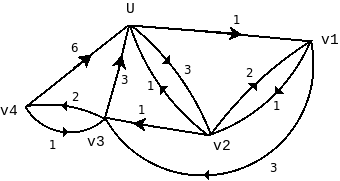
\includegraphics[scale=0.49]{Figura1_11.png}
}
\end{center}
\begin{table}[!hbt]
\begin{tabular}{p{1.5cm}l|c c c c c c p{1cm}c}
Iteración & $v^{'}$ & $L(u)$ & $L(v_1)$ & $L(v_2)$ & $L(v_3)$ & $L(v_4)$ & $T$ \\
\hline
0 & ~--- & 0 & 1 & 3 & $\infty$ & 6 & $\{u\}$ \\
1 & $v_1$ & 0 & 1 & 2 & 4 & 6 & $\{u,v_1\}$ \\
2 & $v_2$ & 0 & 1 & 2 & 3 & 6 & $\{u,v_1,v_2\}$ \\
3 & $v_3$ & 0 & 1 & 2 & 3 & 5 & $\{u,v_1,v_2,v_3\}$ \\
4 & $v_4$ & 0 & 1 & 2 & 3 & 5 & $V$\\
\end{tabular}
\end{table}
\hrulefill{}\\
El algoritmo de Dijkstra determina el camino más corto de $u$ a todos los otros vértices del grafo. Si simplemente estamos interesados en encontrar la distancia más corta desde $u$ hasta cualquier otro vértice especificado $t$, entonces la declaración comenzaría en la línea 4 y se podría terminar tan pronto como $T$ incluya a $t$. Por supuesto, esto no afectaría al \emph{orden} de complejidad de la computación.

Volvemos nuestra atención ahora sobre el segundo ejemplo. Como dijimos anteriormente, su función era encontrar la \emph{máxima} longitud del camino simple entre dos vértices específicados,$u$ y $t$, de un grafo. Cualquier camino simple entre $u$ y $t$ pertenece a un subconjunto de aristas del grafo. En el algoritmo de la Figura1.12 se enumeran todos los subconjuntos de $A$ y a su vez, para aquellos que representan un camino, un registro actual de la trayectoria más larga. Es fácil comprobar que $A^{'}$ es un camino simple desde $u$ hasta $t$ en tiempo polinómico. Esta comprobación se ejecuta para cada iteración de la instrucción en el algoritmo. Sin embargo, hay $2^{|A|}$ iteraciones de este tipo (porque hay $2^{|A|}$ subconjuntos de A) y así sin más detalles del algoritmo, podemos ver que es ineficiente.
\vfill
\begin{algorithm}[H]
\caption{Un algoritmo para comprobar el camino más largo}
\BlankLine
\dontprintsemicolon
$MAXP \leftarrow 0$\;
  \For{todo subconjunto $A^{'} \subseteq A$}
  {
  \If{$A^{'}$ es un camino simple desde $u$ hasta $t$}
  {$MAXP \leftarrow$ \If{$w(A^{'} > MAXP$}{$w(A^{'})$}}}
\end{algorithm}

Hemos visto, por los criterios especificados anteriormente, porque un algoritmo es eficiente y otro es ineficiente. En lo que se refiere al segundo problema, se podría mejorar ligeramente la complejidad del algoritmo si empleamos una enumeración más eficiente o directa para los caminos. Sin embargo, ninguna enumeración de un grafo arbitrario esta delimitada polinomicamente. De hecho, no hay ningún algoritmo conocido para este problema que opere en tiempo polinómico.

Es característico de los problemas \emph{NP-completos} que los algoritmos conocidos requieran un número exponencial de ejecuciones para un tiempo de subtarea polinómico. Por ejemplo, en el problema de la decisión que acabamos de mencionar, es fácil comprobar la longitud de un ruta dada en tiempo polinómico, pera hay un número exponencial de estas. Por definición, cualquier problema \emph{NP-completo} puede transformarse en cualquier otro problema de tiempo polinómico. Así, el descubrimiento de un algoritmo en tiempo polinómico garantiza que ese algoritmo existe para cualquier otro problema.

\section[Estructuras de datos y Búsqueda en Prof.]{Introducción a estructuras de datos y búsqueda en profundidad}

Aquí profundizamos en el concepto de representaciones elementales de grafos para fines computacionales. También describimos un método eficiente para el recorrido de grafos, llamadao búsqueda en profundidad.

\subsection{Matrices de adyacencia y listas de adyacencia}

Las estructuras de datos expuestas aquí se utilizan para representar grafos. En particular, en el uso de listas de adyacencia ya que realizan una importante contribución a la eficiencia de un algoritmo. Una \emph{matriz de adyacencia} para el grafo $G = (V,A)$ es una matriz de $n$ x $n$ $M$, tal que:
\begin{subequations}
\begin{center}
\begin{align}
M(i,j) & = 1 \qquad si \quad (i,j) \in A \nonumber\\
& = 0 \qquad en\quad otro \quad caso \nonumber
\end{align}
\end{center}
\end{subequations}
Si G es un grafo no dirigido entonces $M(i,j) = M(j,i)$, mientras que si G es un dígrafo entonces $M$ es generalmente asimétrico. En la Figura1.13 se ilustran los dos casos. Una especificación de $M$ exige de $O(n^2)$ pasos. Esto elimina cualquier posibilidad de algoritmos de $O(|A|)$ si M representa un grafo disperso, que es aquel en el que el cociente $\frac{|A|}{n}$ es pequeño. Sin embargo, como veremos, los algoritmos $O(|A|)$ son posibles en algunos casos, haciendo uso de \emph{listas de adyacencia}.

En una representación de la lista de adyacencia de un grafo, cada vértice tiene asociada una lista de sus vértices adyacentes. Algunos ejemplos se muestran en la Figura1.13. Estas listas pueden ser incorporadas en una tabla $T$, ejemplos que también se muestran en el diagrama. Con el fin de rastrear la lista de $v_i$, por ejemplo, en la tabla, podemos observar $T(i,2)$ que apunta a $T(T(i,2),1)$, donde el primer vértice adyacente a $v_i$ es registrado. Entonces, $T(T(i,2),2)$ apunta a $T(T(T(i,2),2),1)$ cuando el segundo vértice adyacente a $v_i$ es registrado, y así sucesivamente. La lista de $v_i$ termina cuando se encuentra un puntero nulo.

Claramente, $T$ tiene $(n + |A|)$ filas para un grafo dirigido, y $(n + 2|A|)$ filas para un grafo no dirigido. En algunas circunstancias, es útil, además de utilizar listas doblemente enlazadas para los grafos no dirigidos, también se pueden conectar las dos ocurrencias de una arista $(u,v)$, la primera en la lista de adyacencia de $u$ y la segunda en $v$.

En relación con las matrices de adyacencia hemos de tomar nota de los siguientes teoremas. Este se refiere al producto matricial $k$-ésimo, $M^k$, de la matriz de adyacencia, que se define inductivamente como sigue:
\[M^{k}(i,j) = \sum_{s=1}^{n} M^{k-1}(i,s) M(s,j) \]
donde
\[M^{1}(i,j) = M(i,j) \]
\vfill
\pagebreak
\begin{figure}[H]
\caption{(a) Un dígrafo $G_1$, de su matriz de adyacencia $A_1$ y listas de adyacencia con su representación tabular $T_1$. (b) Un grafo no dirigido $G_2$, de su matriz de adyacencia $A_2$ y listas de adyacencia con su representación tabular}
\hrulefill{}\\
\begin{flushleft}\textbf{(a)}\end{flushleft}
\parbox{1cm}
{
  \begin{flushright}
  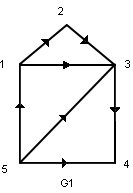
\includegraphics[scale=0.61]{Fig1_13_a.png}
  \end{flushright}
}
\hfill
\parbox{3cm}
{
   \begin{flushleft}
    \[A_1 = \left| 
      \begin{array}{ccccc}
        0 & 1 & 1 & 0 & 0 \\
        0 & 0 & 1 & 0 & 0 \\
        0 & 0 & 0 & 1 & 0 \\
        0 & 0 & 0 & 0 & 0 \\
        1 & 0 & 1 & 1 & 0 \\
      \end{array}
    \right|
    \]
  \end{flushleft}
}
\vfill
\parbox{3cm}
{
  \begin{flushleft}
    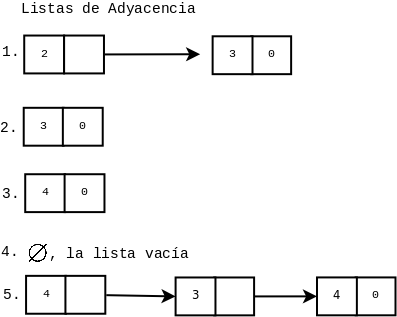
\includegraphics[scale=0.35]{Fig1_13_a3.png}
  \end{flushleft}
}
\hfill
\parbox{2cm}
{
  \begin{flushright}
    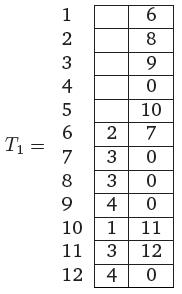
\includegraphics[scale=0.6]{tablita.png}
  \end{flushright}
}
\end{figure}
\hrule
\nopagebreak
\begin{figure}[H]
\begin{flushleft}\textbf{(b)}\end{flushleft}
\parbox{1cm}
{
  \begin{flushright}
  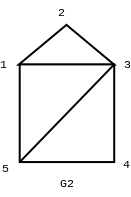
\includegraphics[scale=0.5]{Fig1_13_b.png}
  \end{flushright}
}
\hfill
\parbox{3cm}
{
  \begin{flushleft}
    \[A_2 = \left| 
      \begin{array}{ccccc}
        0 & 1 & 1 & 0 & 1 \\
        1 & 0 & 1 & 0 & 0 \\
        1 & 1 & 0 & 1 & 1 \\
        0 & 0 & 1 & 0 & 0 \\
        1 & 0 & 1 & 1 & 0 \\
      \end{array}
    \right|
    \]
  \end{flushleft}
}
\vfill
\parbox{3cm}
{
  \begin{flushleft}
    \hspace*{-.8in}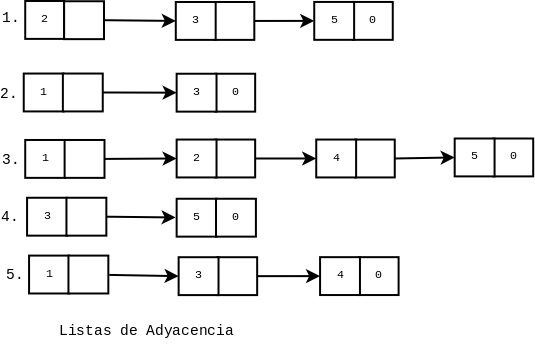
\includegraphics[scale=0.35]{Fig1_13_b3.png}
  \end{flushleft}
}
\hspace*{2in}
\hfill
\parbox{2cm}
{
  \begin{flushright}
    \hspace*{-.2in}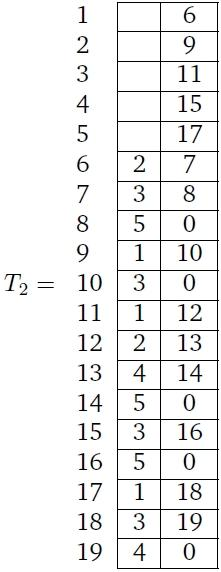
\includegraphics[scale=0.51]{tablita_2.png}
  \end{flushright}
}
\end{figure}
\hrule
\begin{teorema}
$M^k(i,j)$ es el número de caminos (no simples) de $i$ a $j$, que contiene $k$ aristas.
\end{teorema}
\begin{proof}
Por inducción sobre $k$. Si $k = 1$, entonces $M^k(i,j) = 1$ si $(i,j)$ existen y son cero en caso contrario. Así pues, tenemos una base para la inducción. Suponemos que el teorema es cierto para todos los valores de $M$ menos para el $k$-ésimo. Ahora, por definición:
\[M^{k}(i,j) = \sum_{s=1}^{n} M^{k-1}(i,s) M(s,j) \]
y por la hipótesis de inducción $M^{k-1}(i,s)$ es el número de caminos desde $i$ a $s$ y de longitud $(k-1)$. Así que $M^{k-1}(i,s) M(s,j)$ es el número de caminos de longitud $k$ desde $i$ a $j$ que tienen como arista final $(s,j)$. La suma es sobre todos los posibles vértices adyacentes de $j$ y por lo tanto el siguiente resultado.\end{proof}

Antes de llegar a una descripción sobre la búsqueda en profundidad, describiremos un método matricial para encontrar el camino más corto entre cada par de vértices en un grafo ponderado. Esto es en contraste con el algoritmo de Dijkstra que hemos descrito anteriormente, ya que este encuentra el camino más corto desde un vértice especificado a todos los demás. El algoritmo comienza con una matriz $W$ para la que $W(i,j)$ es es el peso $w((v_i,v_j))$, de la arista $(v_i,v_j)$. Si $v_i$ y $v_j$ son distintos y $(v_i,v_j) \notin A$ entonces $w((v_i,v_j)) = \infty $, mientras que $w((v,v)) = 0$. Luego de una serie de matrices $W_1, W_2, \ldots, W_n$ se construyen de acuerdo a la siguiente regla inductiva:
\[ W_k(i,j) = min (W_{k-1}(i,j), (W_{k-1}(i,k) + W_{k-1}(k,j))) \]
donde
\[ W_0(i,j) = W(i,j) \]
$W_n$ proporciona el resultado deseado de acuerdo al siguiente teorema:
\begin{teorema}
$W_n(i,j)$ es la longitud de la ruta más corta de $v_i$ a $v_j$.
\end{teorema}
\begin{proof}
En primer lugar, demostrar por inducción sobre $k$, que $W_k(i,j)$ es el camino más corto desde $v_i$ a $v_j$ que solamente pasan por los vértices del subconjunto $\{v_1, v_2, \ldots, v_k\}$. Si $k = 0$ entonces $W_k(i,j) = w((v_i,v_j))$, de modo que $W_k(i,j)$ es la longitud de la ruta (si existe) de $v_i$ hasta $v_j$ que pasa a través de ningún otro vértice. Suponemos que el enunciado es verdadero para $W_{k-1}(i,j)$. Ahora $W_k(i,j)$ es el más pequeño de $W_{k-1}(i,j)$ y $(W_{k-1}(i,k) + W_{k-1}(k,j))$. En la hipótesis de inducción $W_{k-1}(i,j)$ es el camino más corto desde $v_i$ hasta $v_j$ pasando solo a través de los vértices del subconjunto $V^{'} = \{v_1, v_2, \ldots, v_{k-1}\}$. Si hay una ruta más corta que utiliza $v_k$ así como los vértices de $V^{'}$ entonces su longitud, por la hipótesis de inducción debe ser $(W_{k-1}(i,k) + W_{k-1}(k,j))$. Así pues, el siguiente paso de inducción.\end{proof}

La Figura1.14 muestra que este algoritmo puede ser aplicado para ejecuciones en tiempo $O(n^3)$. La complejidad está dominada por el anidado de las declaraciones en las líneas 2 a 5. Tenga en cuenta que el espacio que emplea el algoritmo como se indica en la Figura 1.14 puede mejorarse considerablemente (sin perjudicar al tiempo) por el reconocimiento de que $W_k$ sólo es necesario para el cálculo de $W_{k+1}$ y no para $W_{k+2}, \ldots, W_n$.\\
\begin{algorithm}[H]
\caption{ }
\BlankLine
\dontprintsemicolon
Inicializo $W_0$\;
\For{$k = 1$ \emph{\KwTo} $n$}
{
  \For{$i = 1$ \emph{\KwTo} $n$}
  {
    \For{$j = 1$ \emph{\KwTo} $n$}
    {
      $W_k(i,j)\leftarrow min((W_{k-1}(i,k) + W_{k-1}(k,j)), W_{k-1}(i,j))$\;
    }
  }
}
Salida $W_n$\;
\end{algorithm}
\subsection{Búsqueda en profundidad}
La mayoría de los algoritmos de grafos requieren un método sistemático para visitar los vértices de un grafo. Una búsqueda en profundidad \emph{(DFS- depth-first search)} es sólo un método que, como veremos, tiene ciertas características que hace posible que algunos algoritmos especialmente eficientes.

El paso general en la búsqueda exige que en la próxima visita a un vértice adyacente a $v$ este aún no haya sido visitado. Si no hay ningún vértice entonces la búsqueda devuelve al vértice visitado justo antes de $v$ y el paso general se repite hasta que todos los vértices de esa componente del grafo haya sido visitado. Esta búsqueda no puede volver a un vértice, excepto por las aristas visitadas anteriormente para llegar a dicho vértice. Por lo tanto las aristas recorridas en la búsqueda en profundidad formar un árbol de expansión para cada componente por separado del grafo. Este conjunto de árboles se le conoce como bosque de expansión por profundidad,$F$. Así, una partición de aristas de $DFS$ en dos grupos, $F$ y $R = A - F$. Las aristas en $R$ son llamadas, \emph{aristas de retroceso}.

Antes de proporcionar un ejemplo de un DFS de un grafo se describe el método en términos de nuestro lenguaje algorítmico. Esto se logra a través del procedimiento recursivo empleado en la Figura 1.15. La entrada a este programa consta de una lista de adyacencia $Ad(v)$ para cada vértice $v$ de $G$. La salida será el conjunto de aristas $F$. El algoritmo utiliza una etiqueta $DFI(v)$ para cada vértice $v$. Llamaremos $DFI(v)$ a la \emph{profundidad del primer índice} de $v$
\vfill
\pagebreak
\begin{algorithm}[H]
\caption{Una búsqueda en profundidad de $G = \{Ad(v)|v \in V\}$ donde $Ad(v)$ es la lista de adyacencia para $v$.}
\dontprintsemicolon
\textbf{procedure} $DFS(v)$
\Begin{
  $DFI(v) \leftarrow i$\;
  $i \leftarrow i + 1$\;
  \For{todo $v^{'} \in Ad(v)$}
  {
    \If{$DFI(v^{'}) = 0$}
    {
      \Begin{
        $F \leftarrow F \cup \{(v,v^{'})\}$\;
        $DFS(v^{'})$\;
      }
     }
   }de $DFS$\;
   $i \leftarrow 1$\;
   $F \leftarrow \emptyset $\;
   \For{todo $v \in V$}
   {
     $DFI(v) \leftarrow 0$\;
   }
   \While{para cualquier $u$, $DFI(u) = 0$}
   {
     $DFS(u)$
   }
   Salida $F$\;
 }
\end{algorithm}

\begin{teorema}
Después de una búsqueda en profundidad de un grafo no dirigido cada una de las aristas de retroceso $(u,v)$, conectando un ancestro con un descendiente.
\end{teorema}
\begin{proof}
Podemos, sin perder la generalidad, suponer que en un $DFS$\footnote{bosque de búsqueda en profundidad} $u$ es visitado antes que $v$. Así $DFS(u)$ se llamaría antes $DFS(v)$ y $DFI$\footnote{profundidad del primer índice}$(v) = 0$ cuando se visita $u$. Todos los vértices visitados durante la ejecución de $DFS(u)$ se convierten en descendientes de $u$. A partir de que $u$ este en la lista de adyacencia de $v$, $DFS(u)$ no terminará antes de que $v$ haya sido visitado y así queda el teorema demostrado.
\end{proof}
En la Figura 1.16 se muestra una aplicación del algoritmo de $DFS$ y una ilustración del teorema 1.6.

La complejidad del algoritmo $DFS$ es $O(max(n,|A|))$ por lo siguiente. Para cada $v \in V$, $DFS(v)$ es llamado una sola vez, porque después de la primera ejecución $DFI(v) = 0$. Además de las llamadas recursivas de $DFS$, el tiempo dedicado por $DFS(v)$ es proporcional a $g(v)$, o para los grafos dirigidos $g^+(v)$. Así, las llamadas de $DFS$ toman un tiempo proporcional a $|A|$. En cambio el orden, en la línea 10, requiere de $O(n)$ pasos al igual que la búsqueda de componentes sucesivos del grafo en la línea 11. La línea 13 requiere $O(|A|)$ pasos.
\vfill
\pagebreak
\begin{figure}[H]
\caption{Un ejemplo que ilustra una aplicación del algoritmo $DFS$.(a)El grafo de dos componentes, cuyas listas de adyacencia cuando son procesadas por el algoritmo $DFS$, producen la salida de abajo. (b)La expansión de los bosques F (en líneas continuas) de salida del algoritmo $DFS$. Las aristas de retroceso se muestran con líneas discontinuas.(c)La profundidad de los vértices ordenados.}
\hrulefill{}\\
\begin{flushleft}\textbf{(a)}\end{flushleft}
\centering
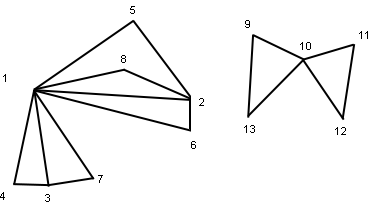
\includegraphics[scale=0.6]{Fig_1_16_a.png}
\end{figure}
\hrulefill{}\\
\parbox{6cm}
{
  \begin{flushleft}\textbf{(b)}\end{flushleft}
  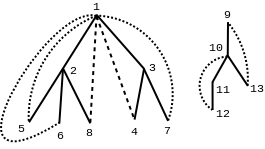
\includegraphics[scale=0.45]{Fig1_16_b.png}
}\parbox{4cm}
{
  \begin{flushleft}\textbf{(c)}\end{flushleft}
  \begin{tabular}{|r|c|}
  \hline
  $v$ & $DFI$ \\
  \hline
  1 & 1 \\
  \hline
  2 & 2 \\
  \hline
  3 & 6 \\
  \hline
  4 & 7 \\
  \hline
  5 & 3 \\
  \hline
  6 & 4 \\
  \hline
  7 & 8 \\
  \hline
  8 & 5 \\
  \hline
  9 & 9 \\
  \hline
  10 & 10 \\
  \hline
  11 & 11 \\
  \hline
  12 & 12 \\
  \hline
  13 & 13 \\
  \hline
\end{tabular}
}\\

\hrule
\vfill
\begin{figure}[H]
\caption{Un ejemplo que ilustra una aplicación del algoritmo $DFS$ a un dígrafo. (a) Un dígrafo que somete al algoritmo $DFS$, produciendo la salida de abajo. (b) El bosque de expansión obtenido se muestra con líneas continuas. Retroceso, directas y cruces de aristas son mostradas en líneas discontinuas. (c) La profundidad de los vértices en orden.}
\hrulefill{}\\
\begin{flushleft}\textbf{(a)}\end{flushleft}
\centering
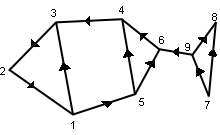
\includegraphics[scale=0.7]{Fig1_17_a.png}
\end{figure}
\hrulefill{}\\
\parbox{6cm}
{
  \begin{flushleft}\textbf{(b)}\end{flushleft}
  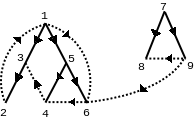
\includegraphics[scale=0.6]{Fig1_17_b.png}
}\parbox{4cm}
{
  \begin{flushleft}\textbf{(c)}\end{flushleft}
  \begin{tabular}{|r|c|}
  \hline
  $v$ & $DFI$ \\
  \hline
  1 & 1 \\
  \hline
  2 & 3 \\
  \hline
  3 & 2 \\
  \hline
  4 & 5 \\
  \hline
  5 & 4 \\
  \hline
  6 & 6 \\
  \hline
  7 & 7 \\
  \hline
  8 & 8 \\
  \hline
  9 & 9 \\
  \hline
\end{tabular}
}\\
\\$F = \{(1,3),(3,2),(1,5),(5,4),(5,6),(7,8),(7,9)\}$ \quad $B_1 = \{(2,1)\}$ 
$C = \{(4,3),(6,4),(9,8),(9,6)\}$ \quad $B_2 = \{(1,6)\}$\\
\hrule

La Figura 1.17 ilustra una aplicación del algoritmo $DFS$. Observe que las particiones de búsqueda de las aristas del grafo son de cuatro tipos:
\begin{description}
\item[\textbf{(i)}] un conjunto de aristas de expansión de un bosque, F,
\item[\textbf{(ii)}] un conjunto de copias de aristas de retroceso, $R_1$, que están dirigidas hacia los descendientes de los ancestros,
\item[\textbf{(iii)}] un conjunto de aristas directas, $R_2$, que están dirigidas a los descendientes de los ancestros,
\item[\textbf{(iv)}] un conjunto de cruces de aristas, $C$, que conectan dos vértices donde ninguno de ellos es descendiente del otro.
\end{description}
A pesar de esta complicación aparente para los dígrafos, en comparación con los grafos no dirigidos, hay un teorema útil análogo al teorema 1.6:
\begin{teorema}
Después de una búsqueda en profundidad de un dígrafo, si $(u,v)$ es un cruce de arista, a continuación, $DFI(u) > DFI(v)$.
\end{teorema}
\begin{proof}
Supongamos que, en contra del teorema, que \\$DFI(u) < DFI(v)$, es decir, $u$ es visitado antes que $v$. Ahora $v$ está en la lista $u$ de adyacencia y por lo tanto deberá ser visitado dentro de $DFS(u)$.Considere el tipo posible de arista $(u,v)$. Si $DFI(v)$ se asigna cuando $(u,v)$ se analiza, entonces $(u,v)$ que deberá ser un bosque de árboles. En caso contrario $v$ es el primero en ser visitado como un descendiente, pero no como hijo de $u$. Entonces $(u,v)$ será una arista directa. Por lo tanto $(u,v)$ no puede ser una arista de cruce y por eso tenemos una contradicción.
\end{proof}

\subsection{Dos algoritmos de tiempo lineal}
A continuación se describe el primer ejemplo de un algoritmo hecho especialmente eficiente en profundidad para una primera búsqueda. Este algoritmo encuentra todos los bloques de un grafo no dirigido dada su lista de adyacencia como entrada. El teorema 1.6 es fundamental para este algoritmo, porque las siguientes observaciones pueden ser hechas como resultado de ello:
Si $v$ es un punto de articulación entonces:
\begin{description}
\item[\textbf{(a)}] Si $v$ es la raíz de un árbol para un bosque de expansión DFS, entonces $v$ tiene más de un hijo.
\item[\textbf{(b)}] Si $v$ no es la raíz de un árbol para un bosque de expansión DFS, entonces $v$ tiene un hijo $v^{'}$ tal que ningún descendiente de $v^{'}$ (incluido $v^{'}$) está conectado por una arista de retroceso hacia un ancestro adecuado de $v$.
\end{description}
Con el fin de identificar los elementos de un grafo, necesitamos identificar sus puntos de articulación y podemos utilizar las observaciones anteriores para hacer esto. A los efectos de implementación \emph{(b)} se asocia con un parámetro $P(v)$ a cada vértice $v$. Si los vértices están etiquetados según el orden en que se visitan en una búsqueda en profundidad, es decir, por $DFI(v)$, entonces $P(v)$ se define como el más pequeño de los vértices $v$ y que están conectados a una arista de retroceso hacia el descendiente de $v$ (incluido $v$). El valor máximo de $P(v)$ es claramente $v$. Teniendo en cuenta esta definición, podemos repetir la observación \emph{(b)}:
Si v es un punto de articulación:
\begin{description}
\item[\textbf{($b^{'}$)}] Si $v$ no es raíz de un árbol para un bosque de expansión DFS, entonces $v$ tiene un hijo $v^{'}$ tal que $P(v^{'}) \ge DFI(v)$.
\end{description}
Utilizaremos el algoritmo $DFS$ como base para el bloque del algoritmo de búsqueda integrado en el seno del cálculo de $P(v)$:
\begin{subequations}
\begin{align}
P(v) = min(\{DFI(v)\} & \cup \{P(v^{'})| v^{'}\quad es\quad un\quad hijo\quad de\quad v\} \nonumber \\
& \cup \{DFI(v^{'}|(v,v^{'}) \in B\}) \nonumber
\end{align}
\end{subequations}

La Figura1.18 incorpora esto dentro del algoritmo $DFS$. La línea 3 de esta búsqueda en profundidad de bloques ($DFSB$) del algoritmo inicializa $P(v)$ a su valor máximo posible $DFI(v)$. En la línea 14 actualizamos $P(v)$ si encontramos un hijo de $v^{'}$ tal que $P(v) \ge P(v^{'})$ y de nuevo $P(v)$ se actualiza en la línea 16 si se encuentra una arista de retroceso adecuada. Los puntos de articulación se identificar a través de la línea 12, cada vez que un vértice $v$ se encuentra tal que $P(v^{'}) \ge DFI(v)$ para algún hijo de $v^{'}$.\\
\vfill
\nopagebreak
\begin{algorithm}[H]
\caption{La búsqueda en profundidad de bloques del algoritmo.}
\BlankLine
\dontprintsemicolon
\textbf{procedure} $DFSB(v)$
\Begin{
  $DFI(v) \leftarrow i$\;
  $P(v) \leftarrow DFI(v)$\;
  $i \leftarrow i + 1$\;
  \For{todo $v^{'} \in Ad(v)$}
  {
    \Begin{
      apilar $(v,v^{'})$ si aún no han sido apilados\;
      \If{$DFI(v^{'}) = 0$}
      {
        \Begin{
          padre $(v^{'}) \leftarrow v$\;
          $DFSB(v)$\;
          \If{$P(v^{'}) \ge DFI(v)$}
          {
            eliminar y extraer de la pila hasta el $(v,v^{'})$\;
            $P(v) \leftarrow$ min $(P(v), P(v^{'}))$\;
          }
        }
      }
      \ElseIf{$v^{'} \ne$ padre $(v)$}
      {
        $P(v) \leftarrow$ min $(P(v), DFI(v^{'}))$\;
      }
    }
  }
  de $DFSB$\;
  $i \leftarrow 1$\;
  vaciar la pila\;
  \For{todo $v\in V$}{$DFI(v) \leftarrow 0$}
  \While{para cualquier $v$, $DFI(v) = 0$}{$DFSB(v)$}
}

\end{algorithm}

El algoritmo de $DFSB$ incorpora una pila que contiene el conjunto de aristas de un bloque extraído tan pronto como se encuentre este. La línea 21 inicializa la pila y la línea 7 la pila de aristas. Tenemos que demostrar que cuando un vértice $v$ y un hijo $v^{'}$ son encontrados tal que $P(v^{'}) \ge DFI(v)$, entonces las aristas de la pila están por encima e incluyen $(v,v^{'})$ definido como un bloque. Esto se demuestra fácilmente por inducción sobre el número de bloques $B$ en un grafo. Si $B = 1$, entonces el único vértice $v$ tal que $P(v^{'} \ge DFI(v)$ es la raíz del árbol $DFS$. Cuando esto se establece, cada extremo del grafo está en la pila con $(v,v^{'})$ en la parte inferior. Así, tenemos una base para nuestra inducción. A partir de nuestra hipótesis de inducción suponemos que el enunciado es verdadero para todos los grafos con menos de $B$ bloques. Consideremos ahora un grafo con $B$ bloques y sea $v$ el primer vértice para el que se encontró que $P(v^{'}) \ge DFI(v)$. No hay aristas que se hayan eliminado de la pila y los elementos de la cima $(v,v^{'})$ deben ser incidentes con los vértices que son descendientes de $v^{'}$. Dado que $v$ es un punto de articulación con ningún descendiente que sea punto de articulación, por encima de las aristas y como $(v,v^{'})$ está en la pila sólo podemos definir el bloque contenedor de $(v,v^{'})$. Cuando las aristas de este bloque se quitan de la pila, el algoritmo se comporta exactamente como lo haría para el grafo con $(B-1)$ bloques obtenido mediante la supresión de los bloques que contienen $(v,v^{'})$. Esto completa el paso inductivo de la demostración.

En la Figura 1.19 se muestra una aplicación de búsqueda en profundidad de bloques del algoritmo. En \textbf{(a)} el grafo sujeto al algoritmo se muestra como si fuera el árbol de expansión, y los valores de $DFI(v)$ y $P(v)$ encontrados durante el curso de la computación. En \textbf{(b)} se ilustra el estado de la pila justo antes y después de las tres ocasiones en que se encuentra un vértice $v$ para el que $P(v^{'}) \ge DFI(v)$ para algún hijo de $v^{'}$.

La complejidad de la búsqueda en profundidad de bloques del algoritmo es $O(max(n,|A|))$. Esto se sigue por una simple extensión de los argumentos utilizados por la complejidad del algoritmo $DFS$. La única complicación surge de la utilización de una pila. Es evidente, sin embargo, que el tiempo total requerido en todas las llamadas del procedimiento $DFSB$ para apilar y posteriormente desapilar aristas es $O(|A|)$. Así, el algoritmo es especialmente eficiente, operando en el tiempo lineal. Esta eficiencia se logra a través de la eficiencia del algoritmo $DFS$ y la característica expresada en el teorema 1.6.
\vfill
\pagebreak
\begin{figure}[H]
\caption{Ilustración de una solicitud de la búsqueda en profundidad de bloques del algoritmo de la figura 1.18}
\end{figure}
\hrulefill{}\\
\begin{center}
\parbox{2cm}
{
  \begin{flushleft}\textbf{(a)}\end{flushleft}
  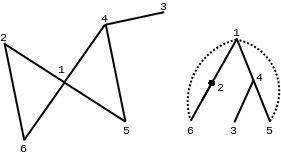
\includegraphics[scale=0.45]{Fig1_19_a.png}
}\hfill
\parbox{4cm}
{
  \begin{flushright}
  \begin{tabular}{|c|c|c|}
  \hline
  $u$ & $DFI$ & P\\
  \hline
  1 & 1 & 1 \\
  \hline
  2 & 2 & 1 \\
  \hline
  3 & 5 & 5 \\
  \hline
  4 & 4 & 1 \\
  \hline
  5 & 6 & 1 \\
  \hline
  6 & 3 & 1 \\
  \hline
\end{tabular}
\end{flushright}
}\\
\end{center}
\hrule
\begin{figure}[H]
\begin{flushleft} \textbf{(b)} \end{flushleft}
\begin{center} Extracción de la pila en la línea 12 \hspace*{0.25in} Bloque de búsqueda\end{center}
\begin{center}
\parbox{3cm}
{
  \textbf{(i)}\\
    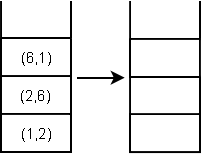
\includegraphics[scale=0.5]{Fig1_19_b1.png}
}
\hspace*{1in}
\parbox{2cm}
{
$ [(6,1),(2,6),(1,2)] $
}
\end{center}
\begin{center}
\parbox{3cm}
{
  \textbf{(ii)}\\
    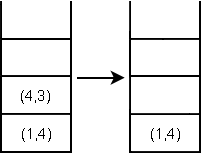
\includegraphics[scale=0.5]{Fig1_19_b2.png}
}
\hspace*{1in}
\parbox{2cm}
{
$ [(4,3)] $
}
\end{center}
\begin{center}
\parbox{3cm}
{
  \textbf{(iii)}\\
    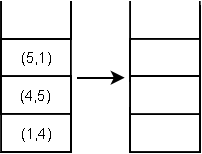
\includegraphics[scale=0.5]{Fig1_19_b3.png}
}
\hspace*{1in}
\parbox{2cm}
{
$ [(1,4),(4,5),(5,1)] $
}
\end{center}

\textbf{(i)} Se produce dentro de $DFSB(1)$ después de la finalización de $DFSB(2)$, que contiene una llamada anidada de $DFSB(6)$.
\textbf{(ii)} Se produce dentro de $DFSB(4)$ (que está anidado dentro de $DFSB(1)$) después de la finalización de $DFSB(3)$.

\textbf{(iii)} Se produce dentro de $DFSB(1)$ después de la finalización de $DFSB(4)$, que contiene una llamada de $DFSB(3)$ y una llamada de $DFSB(5)$.

\hrulefill{}\\
\end{figure}


Llegamos ahora a nuestro segundo ejemplo de un algoritmo hecho especialmente eficiente para una primera búsqueda en profundidad.

\begin{teorema}
Si $G_i = (V_i, A_i)$ es una componente fuertemente conectada del dígrafo $G$ y $F = (V_F,A_F)$ es un bosque de expansión, entonces $T_i = (V_i, A_i \cap A_F)$ es un árbol.
\end{teorema}
\begin{proof}
En primer lugar, demostrar que cualquiera de los dos vértices $u,v \in V_i$ tienen un ancestro común en $V_i$. Supongamos, sin pérdida de generalidad, que $DFI(u) < DFI(v)$. Desde que $u$ y $v$ pertenecen a la misma componente fuertemente conexa, existe un camino $P$ desde $u$ hasta $v$. Se define $w$ como un vértice en $P$ tal que $DFI(w) < DFI(x)$ para cualquier otro vértice $x$ en $P$. Si hacemos una traza $P$ desde $u$, entonces tan pronto como llegemos a $w$, $P$ sólo podrá pasar a través de los vértices que son descendientes de $w$. Esto se debe a que las aristas de los descendientes de $w$ a los vértices que no son descendientes de $w$ son cualquier arista de cruce o arista de retroceso, y ambos serán los vértices con menor profundidad de los primeros índices posibles. Así, $w$ es un ancestro de $v$. También desde que $DFI(w) \le DFI(u) < DFI(v)$, $u$ sólo puede ser un descendiente de $w$.

Sea $r$ la raíz del subárbol que contiene cada vértice en $V_i$. Si $x \in V_i$ y si $y$ están en el camino del árbol desde $r$ hasta $x$, entonces podemos completar la demostración mostrando que $y \in V_i$.
\end{proof}

La raíz del árbol $T$ en el enunciado del teorema 1.8 se llama la \emph{raíz de la componente fuertemente conexa} $G_i$, y se denota por $r_i$. De paso, señalar que el vértice de $G_i$ es su raíz y está en función de que las aristas sean aristas de un árbol. Un dígrafo proporciona, por supuesto, un número de posibles bosques de expansión por profundidad.

El teorema 1.8 sugiere una forma natural para determinar los componentes fuertemente conexos de un dígrafo $G$. Encontramos las raíces, $r_1, r_2, \ldots, r_k$, que convenientemente están en orden de modo que si $i < j$, $r_i$ es visitado por última vez en un primer recorrido en profundidad de $G$ antes de que $r_j$ sea el último visitado. Por el teorema 1.8 y porque $r_j$ no puede ser un descendiente de $r_i$ si $DFI(r_i) > DFI(r_j)$, deducimos que $G_i$ es el subgrafo inducido por los vértices que son descendientes de $r_i$ pero que no son descendientes de $r_1, r_2, \ldots, r_{i-1}$.

De la misma manera que definimos el parámetro $P(v)$ para ayudar en el descubrimiento del cálculo de los puntos de articulación en los grafos no dirigidos, se define un parámetro $Q(v)$ para ayudar en la identificación del cálculo de las ráices de las componentens fuertemente conexas de un dígrafo.
\begin{enumerate}
\item[] \hspace*{0.05in} $Q(v) = min(\{DFI(v)\} \cup \{DFI(v^{'})|(x,v^{'})$ está en $B_1$
\item[] \hspace*{0.1in} o $C$, x es un descendiente de $v$ y la raíz, $r$, de la
\item[] \hspace*{0.1in} componente fuertemente conexa $v^{'}$ es un ancestro
\item[] \hspace*{0.1in} de $v)\}$
\end{enumerate}

El valor de esta definición se encuentra en el siguiente teorema.
\begin{teorema}
En un dígrafo $G$, $v$ es la raíz de una componente fuertemente conex si y sólo si $Q(v) = DFI(v)$.
\end{teorema}
\begin{proof}
Tenga en cuenta que, por definición \\$Q(v) \le DFI(v)$.
En primer lugar, demostrar que si $v$ es la raíz de una componente fuertemente conexa entonces $Q(v) = DFI(v)$. Supongamos que, por el contrario, $Q(v) < DFI(v)$. Por lo tanto, existe un vértice $v^{'}$, como en la definición $Q(v)$, de tal manera que $DFI(v^{'}) < DFI(v)$. Ahora $DFI(r) < DFI(v^{'})$, de modo que tenemos $DFI(r) < DFI(v)$. Pero $r$ y $v$ deben pertenecer a la misma componente fuertemente conexa porque hay un camino de $r$ a $v$ y un camino desde $v$ hasta $r$ a través de $(x,v^{'})$. Así, desde $DFI(r) < DFI(v)$, $v$ no puede ser la raíz de una componente fuertemente conexa. Esta es una contradicción y así llegamos a la conclusión de que $Q(v) = DFI(v)$.

Ahora sólo necesitamos demostrar que si $v$ no es la raíz de una componente fuertemente conexa entonces $Q(v) < DFI(v)$. Supongamos, sin embargo, que $Q(v) = DFI(v)$, de modo que no es un vértice $v^{'}$, como se describió en la definición de $Q(v)$, por lo tanto debería existir para aquellos que $DFI(v^{'} < DFI(v)$. Como $v$ no es la raíz, algunos de los otros vértices $r$ deberá ser la raíz. Entonces debe existir un camino $P$ de $v$ a $r$ que contenga un primer vértice (quizás $r$), que no sea un descendiente de $v$. Permitamos que este vértice sea $v^{'}$. Claramente, $r$ y $v^{'}$ pertenecen a la misma componente fuertemente conexa. La arista de $P$ incidente con $v^{'}$ está en $B_1$ o $C$. Así que $DFI(v^{'}) < DFI(v)$, que es una contradicción. Por lo tanto $Q(v) < DFI(v)$.
\end{proof}
Una vez más se utiliza el algoritmo $DFS$ como base e inserción dentro del cálculo de $Q(v)$. Al igual que con $P(v)$ del ejemplo anterior, se requiere un método recursivo de evaluación para $Q(v)$.
\begin{enumerate}
\item[] \hspace*{0.05in}$Q(v) = min(\{DFI(v)\} \cup \{Q(v^{'})|v^{'}$ es un hijo de $v\}$
\item[] \hspace*{0.1in} $\cup \{DFI(v^{'})|(v,v^{'})$ está en $B_1$ o $C$, de forma que
\item[] \hspace*{0.1in} la raíz de la componente fuertemente conexa 
\item[] \hspace*{0.1in} con $v^{'}$ sea un ancestro de $v$.
\end{enumerate}
En la Figura1.20 incorpora dentro el algoritmo $DFS$. El procedimiento modificado $DFSSCC(v)$\footnote{depth-first search for strongly connected component}, búsqueda en profundidad de los componentes fuertemente conexos, incluye una pila en la que los vértices se sitúan en la línea 5. Una matriz llamada \emph{apilada} se utilizar para registrar los vértices que están en la pila. La línea 3 inicializa $Q(v)$ a su máximo valor posible y la línea 10 actualiza $Q(v)$ si se encuentra un hijo de $v$,$v^{'}$, tales que $Q(v^{'}) < Q(v)$. La línea 12 actualiza nuevamente $Q(v)$ si una arista $(v,v^{'})$ en $B_1$ o $C$ se encuentra de tal manera que la raíz de la componente fuertemente conexa $v^{'}$ es un ancestro de $v$. Tenga en cuenta que en la línea 12 $DFI(v^{'}) \ne 0$ y así $v^{'}$ ha sido visitado anteriormente y a partir de que $DFI(v^{'}) < DFI(v)$ tendrá lugar la actualización de $(v,v^{'})$ que no podrá ser una arista directa. Además, dado que se apila $v^{'}$, la raíz de la componente fuertemente conexa $v^{'}$ ya se ha identificado y que, por el orden en que se identifican las raíces, debe ser un ancestro de $v$. La línea 15 identifica las raíces, de nuevo por el teorema 1.8 y el orden de identificación de la raíces, los vértices superiores e incluyendo la cima de la pila que debe inducir a una componente fuertemente conexa.
\begin{algorithm}[H]
\caption{La búsqueda en profundidad para el algoritmo de componentes fuertemente conexas.}
\BlankLine
\dontprintsemicolon
\textbf{procedure} $DFSSCC(v)$
\Begin{
  $DFI(v) \leftarrow i$\;
  $Q(v) \leftarrow DFI(v)$\;
  $i \leftarrow i + 1$\;
  poner $v$ en la pila y $apilar(v) \leftarrow \bf{true}$\;
  \For{para $v^{'} \in Ad(v)$}{
    \If{$DFI(v^{'}) = 0$}{
      \Begin{
        $DFSSCC(v^{'})$\;
        $Q(v) \leftarrow$ min($Q(v), Q(v^{'})$)\;
      }
        \Else{\If{$DFI(v^{'}) < DFI(v)$ {\bf{and}} apilar $(v^{'})$}
          {$Q(v) \leftarrow$ min ($Q(v), DFI(v^{'})$)}
        }
      }
    }
    \If{$Q(v) = DFI(v)$}{eliminar y extraer la pila incluido $v$, por cada vértice $u$ restableciendo $apilar(u) \leftarrow false$}(de $DFSSCC$)\;
    $i \leftarrow 1$\;
    vaciar la pila\;
    \For{todo $v \in V$}
    {
      \Begin
      {
        $DFI(v) \leftarrow 0$, $apilar(v) \leftarrow \bf{false}$
      }
    }
    \While{para cualquier $u$, $DFI(u) = 0$}{
      $DFSSCC(u)$
    }
  }
\end{algorithm}
En la Figura 1.21 se muestra una aplicación de búsqueda en profundidad para el algoritmo de componentes fuertemente conexas. En \textbf{(a)} el grafo obtenido del algoritmo muestra como son sus bosques de expansión y los valores de $DFI(v)$ y $Q(v)$ encontrados durante el curso de la computación. En \textbf{(b)} se muestra el estado de la pila justo antes de encontrar un vértice para el que $Q(v) = DFI(v)$ y justo después de que los vértices de una componente fuertemente conexa hayan sido extraídos de la pila. También se indican en cuál de las llamadas recursivas de $DFSSCC$ las componentes se encuentran fuertemente conectadas.

El algoritmo de $DFSSCC$ opera dentro de un tiempo lineal, con complejidad $O(max(n,|A|))$. Esto sigue el argumento similar empleado por el algoritmo de DFSB.
\vfill
\nopagebreak
\begin{figure}[H]
\caption{ }
\end{figure}
\hrulefill{}\\
\begin{center}
\parbox{1cm}
{
  \begin{flushleft}\textbf{(a)}\end{flushleft}
  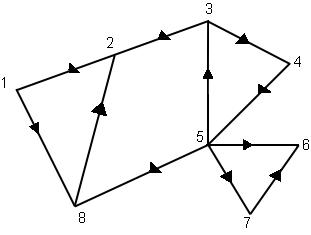
\includegraphics[scale=0.4]{Fig1_21_a1.png}
}\hfill
\parbox{5cm}
{
  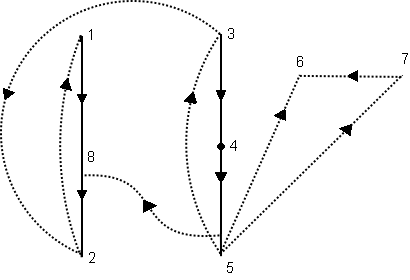
\includegraphics[scale=0.42]{Fig1_21_a2.png}
}\hfill

\parbox{4cm}
{
  \begin{flushright}
  \begin{tabular}{|c|c|c|}
  \hline
  $v$ & $DFI$ & $Q$\\
  \hline
  1 & 1 & 1 \\
  \hline
  2 & 3 & 1 \\
  \hline
  3 & 4 & 4 \\
  \hline
  4 & 5 & 4 \\
  \hline
  5 & 6 & 4 \\
  \hline
  6 & 7 & 7 \\
  \hline
  7 & 8 & 8 \\
  \hline
  8 & 2 & 1 \\
  \hline
\end{tabular}
\end{flushright}
}\\
\end{center}
\hrule
\begin{figure}[H]
\begin{flushleft} \textbf{(b)} \end{flushleft}
\begin{center} Extracción de la pila en la línea 15 \hspace*{0.25in} Inducción de vértices\\ \hspace*{2.4in}por una componente \\ \hspace*{2.4in}fuertemente conexa\end{center}
\begin{center}
\parbox{3cm}
{
  \textbf{(i)}\\
    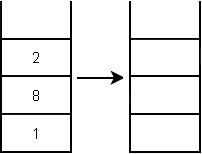
\includegraphics[scale=0.5]{Fig1_21_b1.png}
}
\hspace*{1in}
\parbox{2cm}
{
$ [1,2,8] $
}
\end{center}
\begin{center}
\parbox{3cm}
{
  \textbf{(ii)}\\
    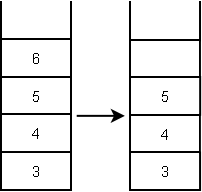
\includegraphics[scale=0.5]{Fig1_21_b2.png}
}
\hspace*{1in}
\parbox{2cm}
{
$ [6] $
}
\end{center}
\begin{center}
\parbox{3cm}
{
  \textbf{(iii)}\\
    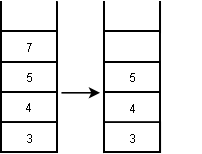
\includegraphics[scale=0.5]{Fig1_21_b3.png}
}
\hspace*{1in}
\parbox{2cm}
{
$ [7] $
}
\end{center}
\begin{center}
\parbox{3cm}
{
  \textbf{(iv)}\\
    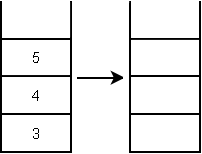
\includegraphics[scale=0.5]{Fig1_21_b4.png}
}
\hspace*{1in}
\parbox{2cm}
{
$ [3,4,5] $
}
\end{center}
\end{figure}

\textbf{(i)} Se produce dentro de $DFSSCC(1)$ después de la finalización de $DFSSCC(8)$ que contiene una llamada anidada de $DFSSCC(2)$.

\textbf{(ii)} Se produce dentro de $DFSSCC(6)$ que está anidado sucesivamente dentro de $DFSSCC(5), DFSSCC(4)$ y $ DFSSCC(3)$.

\textbf{(iii)} Se produce dentro de $DFSSCC(7)$ que se llama inmediatamente después de $DFSSCC(6)$.

\textbf{(iv)} Se produce dentro de $DFSSCC(3)$ que se llama después de la finalización de $DFSSCC(1)$.

\hrulefill{}\\

\chapter[Árbol exp. , ramificacion y conect.]{Árboles de expansión, ramificaciones y conectividad}

Los árboles son el tipo más frecuente de grafos en los modelos y cálculos de todo tipo. Los científicos en computación están particularmente familiarizados con estas estructuras a través de la consideración de árboles de parser, árboles de búsqueda, árboles de juego y así sucesivamente.

\section{Árboles de expansión y ramificación}

Un árbol de expansión de un grafo conectado no dirigido $G$ es un subgrafo que es como un árbol y que contiene todos los vértices de $G$. Como vimos en el capítulo 1, este árbol de expansión se puede encontrar en un tiempo lineal empleando, por ejemplo, una búsqueda en profundidad.

En esta sección se describen en primer lugar un algoritmo que resuelve una tarea más general. Se trata de encontrar, dado un grafo ponderado, conectado y no dirigido, un árbol de expansión de peso mínimo. Este problema puede aparecer en una serie de formas, la más común de lo que se refiere a la construcción de una red de comunicación, tal vez un camino o un sistema ferroviario que une un conjunto de ciudades. Dado el coste de la conexión directa de cualquiera de las dos ciudades, el problema es encontrar una red a un coste mínimo y que proporcione alguna ruta entre las dos ciudades. La solución es el mínimo peso del árbol completo de expansión asociado al grafo. Debido a esta descripción del problema es a menudo llamado el problema del conector. El problema similar de encontrar un peso máximo del árbol de expansión se puede resolver haciendo una pequeña modificación del peso mínimo del algoritmo del árbol de expansión que se describe.

\subsection{Peso óptimo de los árboles de expansión}

Hay una serie de algoritmos conocidos para resolver el problema de conexión para grafos no dirigidos. Los más conocidos de estos son debidos a Prim\cite{d}, que se describe aquí, y de Kruskal.

El algoritmo de Prim se describe en la Figura 2.1. En cada etapa el algoritmo iterativo, una nueva arista $a$ se agrega a $T$. Ahora, $T$ es un subgrafo conexo de peso mínimo del árbol de expansión en construcción, y abarca un subconjunto de vértices $V^{'} \subset V$. La arista $a$ es la arista de peso mínimo de la conexión de un vértice desde ($V - V^{'}$) hacia un vértice de $V^{'}$. Inicialmente $V^{'}$ contiene algunos vértices arbitrarios $u$. En cada etapa, la etiqueta $L(v)$, para cada vértice $v$, recorre la arista de menos peso desde $v \in (V- V^{'})$ a un vértice de $V^{'}$. Así, cada $L(v)$ es inicializado con el peso $w((u,v))$ de la arista $(u,v)$, siempre que $(u,v) \in A$. De lo contrario $w((u,v)) = \infty$ si $u$ y $v$ son distintos, mientras que $w((u,v)) = 0$. La línea 8 del algoritmo actualiza $L(v)$ cuando un nuevo vértice $w$ se ha añadido a $V^{'}$. El algoritmo se detiene cuando $V = V^{'}$, en la línea 4.

\begin{teorema}
El algoritmo de Prim encuentra el peso mínimo del árbol de expansión de un grafo no dirigido conexo $G$.
\end{teorema}
\begin{proof}
Demostraremos por inducción sobre el tamaño de $V^{'}$ dado un subárbol de mínimo peso $T$ del árbol de expansión de $G$ que abarca los vértices de $V^{'}$.

Como base para nuestra inducción, tomamos nota de que la declaración es una verdad trivial cuando $T$ y $V^{'}$ son inicializadas en las líneas 1 y 2 del algoritmo. Suponemos entonces que es cierto, cualquier que sea el valor de $|V^{'}|$, justo antes de que $a$ se añada a $T$ en la línea 6. Consideremos ahora $(T + a)$. En primer lugar, demostrar que $(T + a)$ es un árbol.

La arista $a$ sirve para conectar $w$ con un vértice $v$ de $T$. Dado que la hipótesis de inducción $T$ esta conectada, $(T + a)$ debe serlo también. Ahora $(T + a)$ no puede contener un circuito porque no es $T$ y porque uno de los extremos de $a$, llamado $w$, es de un grado 1 en $(T + a)$. Por lo tanto $(T + a)$ es a la vez conexo y acíclico y consecuentemente debe ser un árbol.

\begin{algorithm}[H]
\caption{Algoritmo de Prim para árboles de expansión de coste mínimo}
\BlankLine
\dontprintsemicolon
$T \leftarrow \emptyset$\;
$V' \leftarrow \{ u \}$\;
\For{todo $v \in (V - V')$}
{
  $L(v) \leftarrow w((u,v))$\;
}
\While{$V' \ne V$}
{
  \Begin{
    encontrar un $w$ para el que $L(w) =$ min$\{L(v)|v \in (V - V')\}$ y denota la asociación de aristas desde $V'$ hasta $w$ por $a$.\;
    $T \leftarrow T \cup \{a\}$\;
    $V' \leftarrow V' \cup \{w\}$\;
    \For{ todo $v \in (V - V')$}
    {
      $L(v) \leftarrow$ \If{$w((v,w)) < L(v)$}{$w((v,w))$}
    }
  }
}

\end{algorithm}

\begin{figure}[H]
  \caption{Una aplicación del algoritmo de Prim. Para cada iteración del bucle mientras $T$ se convierte en $T \cup \{a\}$ y $V'$ se convierte en $V' \cup \{w\}$. Por último, $T$ es el árbol de expansión de peso mínimo compuesto por las aristas de mayor peso}
\end{figure}
\hrulefill{}\\
\begin{center}
  \parbox{1cm}
  {
    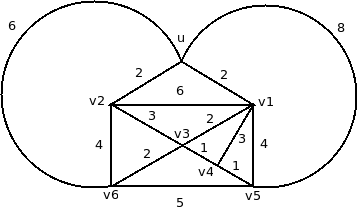
\includegraphics[scale=0.4]{Figura2_2.png}
  }\hfill
  \parbox{3cm}
  {
    \begin{flushright}
      \begin{tabular}{|c|c|c|}
        \hline
        Iteración & $w$ & $a$\\
        \hline
        1 & $v_1$ & $(u,v_1)$ \\
        \hline
        2 & $v_2$ & $(u,v_2)$ \\
        \hline
        3 & $v_3$ & $(v_1,v_3)$ \\
        \hline
        4 & $v_4$ & $(v_3,v_4)$ \\
        \hline
        5 & $v_5$ & $(v_4,v_5)$ \\
        \hline
        6 & $v_6$ & $(v_3,v_6)$ \\
        \hline
      \end{tabular}
    \end{flushright}
  }\\
\end{center}
\hrule


Ahora se demuestra que $(T + a)$ es un subárbol de peso mínimo del árbol de expansión de $G$. En la hipótesis de inducción $T \subset T_M$, donde $T_M$ es un peso mínimo del árbolde expansión de $G$. Supongamos que $a$ no es una arista de $T_M$. Luego, por el teorema\ref{teorema1.2} $(T_M + a)$ contiene un circuito $C$. Una de las aristas de $C$, llamada $a$, conecta un vértice desde $V^{'}$ a un vértice en $(V - V^{'})$. Por tanto, existe otra arista $a^{'}$ desde $V^{'}$ hacia $(V - V^{'})$ en $C$. Si ahora construimos el árbol $T^{'}_M = (T_M + a) - a^{'}$, nos damos cuenta de que $(T + a) \subset T^{'}_M$. Además $T^{'}_M$ es el mínimo peso del árbol de expansión debido a que:
\[ w(T^{'}_M) = w(T_M) + w(a) - w(a^{'})\]
y desde la línea 5 del algoritmo:
\[ w(a) \le w(a^{'})\]
de modo que:
\[ w(T^{'}_M) = w(T_M) \]

Así, cuando $a$ se añade a $T$, $(T + a)$ es todavía un subárbol de peso mínimo del árbol de expansión.

Para terminar el algoritmo, en la línea 4, $V^{'}=V$ de manera que $T$ extiende  $G$.
\end{proof}

El algoritmo de Prim es eficiente, tal como a continuación veremos. El cuerpo del while, desde las líneas 5 a la 8 de la Figura 2.1, se ejecutará $(n-1)$ veces. Dentro de cada ejecución tanto el cálculo de $min\{L(v)|v \in (V - V^{'})\}$ en la línea 5 como la instrucción de la línea 8 pueden ejecutarse dentro de $O(n)$ pasos. Así, en general, tenemos que el algoritmo es $O(n^2)$.

Este algoritmo, como ya hemos descrito, encuentra el mínimo peso del árbol de expansión. Es fácil ver que la simple modificación de sustituir $min\{L(v)\}$ por $max\{L(v)\}$ en la línea 5 hará que el algoritmo encuentre el máximo peso del árbol de expansión.

Lo siguiente es un generalización del peso mínimo que pertenece al problema de los árboles de expansión. Dado un subconjunto propio\footnote{
Sean A y B dos conjuntos tal que todo elemento de A es también de B, entonces decimos que:
\begin{enumerate}
\item A es subconjunto de B $\rightarrow$ $A \subseteq B$;
\item B es un superconjunto de A $\rightarrow$ $B \supseteq A$;
\end{enumerate}
Todo conjunto A es un subconjunto de sí mismo. Cualquier subconjunto de A que no sea igual a A se denomina propio. Si A es un subconjunto propio de B, escribimos:
\[A \subset B\]}, $V^{'}$, de los vértices de un grafo conexo y no dirigido ponderado, encontrar un árbol de peso mínimo que extienda los vertices de $V^{'}$, y si fuera necesario, de algunos otros. Este árbol se llama árbol de Steiner. \textbf{No se conoce ningún algoritmo eficiente} para el problema del árbol de Steiner. De hecho, el problema de decisión relacionado es \emph{NP-completo}.

\subsection{Ramificaciones Óptimas}

En la sección anterior, estábamos preocupados por encontrar árboles ponderados para los grafos no dirigidos. Aquí vemos un problema similar para los dígrafos. Se describe un algoritmo debido a Edmonds\cite{b}. Este encuentra un subgrafo de un dígrafo de máximo peso, lo que no significa necesariamente que sea de expansión, que es un bosque de árboles llamado ramificación máxima. Veremos que el mismo algoritmo, con algunos cambios,se puede utilizar, para encontrar un bosque de árboles llamado esta vez de mínima ramificación.

El algoritmo recorre el dígrafo examinando los vértices y las aristas. Se colocan los vértices en el llamado \emph{cubo de vértices BV}, que ya han sido examinados, y las aristas en el llamado \emph{cubo de aristas BA} si han sido elegido provisionalmente para la ramificación. Consideramos el curso del algoritmo BA que siempre contiene una ramificación, como una colección acíclica de aristas dirigidas con una arista incidente hacia cualquier vértice. El análisis de un vértice $v$ consiste en elegir una arista de máxima peso positivo $a$ que sea incidente a $v$.

Hay que tener en cuenta que ninguna arista de peso negativo será elegida para una máxima ramificación. La arista $a$ se revisa para ver si forma un circuito con las aristas incluidas en $BA$. Si no se puede revisar entonces $a$ se añade a $BA$ y un nuevo vértice se examina. Si se realiza entonces el grafo se reestructura por reducción de este circuito para un solo vértice y la asignación de nuevos pesos a las aristas que son incidentes a este vértice nuevo ``artificial''.

El proceso de inspección de los vértices continua hasta que $BV$ contenga a todos los vértices en un grafo final. Este contiene sólo estos vértices, varios de los cuales en general pueden ser ``artificiales'', porque cada vez que un circuito es reducido para formar un nuevo grafo de aristas y vértices se eliminan de $BA$ y $BV$. $BA$ en esta etapa contiene las aristas de máxima ramificación del grafo final. El proceso inverso de sustitución cambia cada uno de los vértices artificiales creados por su circuito asociado que comienze. En cada una de las sustituciones la elección de las aristas colocadas en $BA$ es tal que para el nuevo grafo reconstruido, $BA$ contiene las aristas para la máxima ramificación. Como veremos, el elemento crucial del algoritmo es la regla para la reasignación de pesos a las aristas cuando se reducen los circuitos.

Un esquema del algoritmo se muestra en la Figura 2.3. El dígrafo original, entrada al algoritmo, es $G_0 = (V_0,A_0)$ y $G_i = (V_i,A_i)$ es el grafo obtenido tras el $i-\acute{e}simo$ circuito que se ha reemplazado por un vértice simple $u_i$. Las líneas 11-13 inclusive generan la sucesión de grafos $G_1,G_2, \ldots, G_K$ siempre que uno o más circuitos tengan que ser educido a los vértices artificiales. Este proceso termina cuando $BV$ contiene las aristas de la gráfica actual en la línea 4. Tenemos que completar los detalles por los que se construye $G_i$ a partir de $G_{i-1}$ y por el cual $BA, BV,$ y cualquier arista son modificadas en las líneas 10 y 11.

Como se puede imaginar $G_i$ contiene cada vértice de $G_{i-1}$, excepto para los de $C_i$. $V_i$ también incluye el nuevo vértice $u_i$. $A_i$ contiene cada arista de $A_{i-1}$ excepto aquellas con uno o más puntos finales en $C_i$. También vamos a añadir a $A_i$ nuevas aristsa de la siguiente manera. Para cada arista $(x,y) \in A_{i-1}$ para los que $x \notin C_i$ e $y \in C_i$ (o para los que $x \in C_i$ e $y \notin C_i$), $A_i$ contiene una arista $(x,u_i)$ (o una arista $(u_i,y)$). Cualquier arista en $G_i$ tiene el mismo peso que su arista correspondiente en $G_{i-1}$, excepto para aquellas aristas incidentes hacia $u_i$. Para cualquiera de las aristas $(x,u_i)$, denotamos su equivalente en $A_{i-1}$ por $a = (x,y)$. Esto define un vértice $y$ en $C_i$ y una única arista $\tilde{a}$ en $C_i$ que es incidente a $y$. Además de definir un mínimo de peso en $C_i$ para $a_i^0$. Entonces, el peso de cada arista $(x,u_i)$ en $G_i$ se define como:

\[ w(x,u_i) = w(a) - w(\tilde{a}) + w(a_i^0) \]

La motivación para esta asignación se hará evidente en el teorema 2.2. $BV$ se modifica simplemente quitando cualquier vértice de $BV$ que podrían estar en $C_i$. $BA$ es modificado mediante la eliminación de las aristas de $C_i$ y sustituyendo estas aristas con un único punto de $C_i$ con sus aristas equivalentes en $A_i$. Observe que el último implicará, en su caso, sólo las aristas incidentes desde $u_i$. Las aristas de máximo peso en los vértices de $C_i$ son en realidad los bordes de $C_i$, de lo contrario $C_i$ no habrían sido identificados. Cuando $u_i$ sea elegida en la línea 4, una arista incidente hacia $u_i$ podría añadirse a $BA$ en la línea 12 si tiene, como se muestra en la línea 7, un peso positivo.

La sentencia repetitiva while de las líneas 14-19, a su vez, es para las aristas de cada circuito $C_k, C_{k-1}, \ldots, C$ que son incluidas en la ramificación. En la línea 15 $G_{i-1}$ se reconstruye desde $G_i$ en la forma obvia (de hecho, un algoritmo detallado en realidad podría mantener $G_{i-1}$ cuando $G_i$ es construido a partir de él). También en la línea 11 las aristas de $BA$ con $u_i$ como un vértice o extremo se sustituirán por su equivalente en 

\vfill
\pagebreak
\begin{algorithm}[H]
\caption{Algoritmo de Edmond para encontrar una ramificación máxima}
\BlankLine
\dontprintsemicolon
$BV \leftarrow BA \leftarrow \emptyset$\;
$i \leftarrow 0$\;
\If{$BV = V_i$}{\textbf{go to} 14}
\For{algún vértice $v \notin BV$ \textbf{and} $v \in V_i$}
{
  \Begin{
    $BV \leftarrow BV \cup \{v\}$\;
    encontrar una arista $a = (x,y)$ tal que $w(a)$ = max\{$(y,v)|(y,v) \in A_i$\}\;
    \If{ $w(a) \le 0$}{\textbf{go to} 3}\;
  }
}
\If{$BA \cup \{a\}$ contiene un circuito}
{
  \Begin{
    $i \leftarrow i + 1$\;
    construir $G_i$ por reducción de $C_i$ a $u_i$\;
    modificar $BA, BV$ y cualquier peso de una arista\;
  }
}
$BA \leftarrow BA \cup \{a\}$\;
\textbf{go to} 3\;
\While{$i\ne 0$}
{
  \Begin{
    reconstruir $G_{i-1}$ y renombrar algunas aristas en $BA$\;
    \eIf{$u_i$ era la raíz de un árbol en $BA$}
    {
      $BA \leftarrow BA \cup \{ a|a \in C_i$ y $a \ne a_0^i \}$\;  
    }
    {
      $BA \leftarrow BA \cup \{a|a \in C_i$ y $a \ne \tilde{a}_i \}$\;
    }

    $i \leftarrow i - 1$\;
  }
  ramificación máxima ponderada $\leftarrow \sum_{a \in BA}^{} w(a)$
}
\end{algorithm}

las aristas de $G_{i-1}$. Qué aristas de cada $C_i$ son añadirán dependerá de si $BA$ contiene una arista incidente hacia un vértice de $C_i$ o no.

Como se indica en la línea 20, el conjunto final de las aristas de $BA$ se define como una máxima ramificación de $G_0$.

\begin{teorema}
El algoritmo de Edmond busca una ramificación máxima para un dígrafo ponderado.
\end{teorema}
\begin{proof}
Vamos a demostrar que si $BA$ contiene las aristas para una máxima ramificación de $G_i$, entonces posteriormente lo para $G_{i-1}$ en la fase de reconstrucción del algoritmo. Si $BA$ contiene las aristas de una máxima ramificación para el grafo más pequeño de $G_k$, entonces tendremos una prueba por inducción que a la larga en $BA$ contendrá las aristas de algunas ramificaciones máximas de $G_0$.

Como base para nuestra inducción consideremos $G_k$ cuando $BV$ contenga todos los vértices de $V_k$, detectados en la línea 3. Luego $BA$ contiene sólo una de las aristsa de máximo peso incidentes a cada vértice de $V_k$, siempre que la arista sea de peso positivo. También las aristas de $BA$ son acíclicas. Evidentemente, $BA$ representa una ramificación máxima de $G_k$.

Ahora $BA$ contiene las aristas de una máxima ramificación de $G_i$. Considere $G_{i-1}$ y los correspondientes conjuntos de aristas $BA$, tal como se definió en la declaración del mientras a partir de la línea 13 del algoritmo. Sea $A'_{i-1}$ el conjunto de las aristas de $G_{i-1}$ que son incidentes a los vértices de $C_i$ y sea $A''_{i-1}$ las aristas restantes de $G_{i-1}$. Denotamos las aristas de $A'_{i-1}$ que se encuentran de $BA$ por $BA'$ y las aristas de $A''_{i-1}$ que se encuentran en $BA$ de $BA''$. Si $BA$ no representa una máxima ramificación de $G_{i-1}$, entonces debe haber una ramificación $B$ con aristas $B'$ en $A'_{i-1}$ y aristas $B''$ en $A''_{i-1}$ tal que:
\begin{description}
\item[] (a) $w(B') > w(BA'')$
\end{description}
ó
\begin{description}
\item[] (b) $w(B'') > w(BA'')$
\end{description}

De hecho, vamos a demostrar que $BA'$ es una máxima ramificación para $A'_{i-1}$ y $w(B'') = w(BA'')$. Considere la posibilidad de $A'_{i-1}$ en primer lugar.

Para cada vértice de $C_i$, la arista de entrada de peso máximo, y que será de peso positivo, es una arista de $C_i$. De lo contrario $C_i$ no habría sido identificado como un circuito. No hay una ramificación máxima de $A'_{i-1}$ que contenga cada arista de $C_i$. Sin embargo, hay una máxima ramificación de $A'_{i-1}$ que incluye a todas menos una arista de $C_i$. Esto es porque, de una ramificación con exclusión de dos o más aristas de $C_i$, siempre se puede obtener una ramificación de peso mayor o igual de la siguiente manera. Sea $v$ un vértice de $C_i$, que no tiene arista en $C_i$ incidente a ella. Entonces cualquier $v$ es una arista de $a$, no de $C_i$, incidente a ella o no. Si $a$ existe entonces es sustituido por otra arista de mayor peso, $\tilde{a}$ es incidente a $v$ y esta en $C_i$, de lo contrario una ramificación de mayor peso de mayor peso se obtiene simplemente como $\tilde{a}$. Ahora consideremos cuál de las ramificaciones de $A'_{i-1}$ con todas menos una arista de $C_i$ son de peso máximo. Cualquier ramificación contrendrá al menos una arista de la forma $a = (x,y), x \notin C_i$ y $y \in C_i$, donde la arista de $C_i$ sería incidente a $y$, $\tilde{a}$, podría estar ausente. Ahora bien, si existe una arista $a$ para una ramificación de $A'_{i-1}$, entonces el peso de las ramas podría ser:
\[w(C_i) + w(a) - w(\tilde{a})\]
Supongamos que $a$ ha sido elegida para maximizar esta expresión. Las ramificaciones que donde no emplean una arista como $a$, tendrán como peso máximo el peso:
\[w(C_i) - w(a_i^0)\]
donde $a_i^0$ es la arista de $C_i$ con el mínimo peso. Así, si
\[w(C_i) + w(a) - w(\tilde{a}) > w(C_i) - w(a_i^0)\]
es decir, si
\[w(a) - w(\tilde{a}) + w(a_i^0) > 0\]
entonces una ramificación de peso máximo de $A'_{i-1}$, que incluye cada arista siendo una de $C_i$, tiene una arista tal como $a$. De lo contrario, no lo haría. El lado izquierdo de la última desigualdad es, precisamente, el peso asignado $a$ cuando $C_i$ es reducido a $u_i$ en el algoritmo. Cuando el algoritmo encuentra una ramificación de $G_i$ entonces $a$ esta en $BA$ si la desigualdad se cumple para la arista de máximo peso incidente con $u_i$. Luego la línea 18 asigna a las aristas de $C_i - \{\tilde{a}\}$ a $BA'$ cuando $u_i$ se extiende a $C_i$ para formar $G_{i-1}$. Si la última desigualdad es válida para cualquier arista $u_i$ de $G_i$, entonces $u_i$ se convierte en la raíz de un árbol en $BA$. La línea 17 del algoritmo asigna las aristas de $C_i - a_i^0$ en $BA$. Así, el algoritmo proporciona una correspondencia máxima para $A'_{i-1}$.

Ahora se demuestra que $w(B'') = w(BA'')$. Sin pérdida de generalidad, podemos suponer que $B'$ es de la forma de $BA'$ por el algoritmo. Si no es así, entonces se puede convertir en una forma tal que no afecte a $B''$. Hay entonces dos casos a considerar:
\begin{description}
\item[(i)] La ramificación de $A'_{i-1}$ no contiene ninguna arista fuera de $C_i$.
\item[(ii)] La ramificación de $A'_{i-1}$ contiene una arista $a= (x,y)$ donde $x \notin C_i$ e $y \in C_i$.
\end{description}

En la hipótesis de inducción $BA$ representa una ramificación máxima para $G_i$ antes de que $u_i$ se extienda a $C_i$. En el caso de \textbf{(i)} esta ramificación máxima tiene una correspondencia uno-a-uno con las aristas de la ramificación producidas por $A''_{i-1}$ por el algoritmo. Así, en este caso $w(B'') = w(BA'')"$. En el caso \textbf{(ii)} la ramificación de $A''_{i-1}$ producido por el algoritmo tiene una correspondencia una-a-una aristas con la ramificación máxima de $G_i$ menos la arista de esta ramificación incidente con $u_i$. Sin embargo, queda claro que $w(B) = w(BA'')$ porque si el peso de las ramas de $A''_{i-1}$ puede aumentarse sin incluir una ruta desde un vértice de $C_i$ a $x$, entonces la ramificación de $G_i$ no sería máxima. Se podría construir otra de mayor peso de esa ramificación con una correspondencia una-a-una aristas con una mayor ramificación de $A''_{i-1}$ más la arista de la ramificación máxima original de $G_i$ en $u_i$.
\end{proof}

En la figura 2.4 se muestra una aplicación del algoritmo de Edmond. Los vértices imaginados deben examinarse en orden alfabético, con los vértices artificiales que son añadidos al final de la cola y en el orden en que son creados. A partir de $G_0$, $(a)$ muestra los sucesivos grafos $G_1$ y $G_2$ obtenidos en la etapa de reducción del circuito del algoritmo. Coincidentemente, ya que en general no sería el caso, $BV$ y $BA$ están vacíos cuando se inici el proceso en $G_1$ y $G_2$. Para $G_0, G_1$ y $G_2$ se muestran los valores finales de $BA$ y $BV$. En la figura 2.4 $(b)$ se muestra el contenido sucesivo de $BA$ como $G_1$ y como se reconstruye $G_0$. Observe que el conjunto final de las aristas de $BA$, que definen una ramificación máxima de $G_0$, es en realidad una sola raíz del árbol en $B$ que no, por cierto, incluye la arista de máximo peso en $G_0$.

El algoritmo de Edmond es eficiente, ya que se ejecuta en un tiempo de $O(n|A|)$. La etapa más costosa concierne a la construcción y reconstrucción de los grafos. Para cada grafo nuevo se requiere $O(|A|)$ pasos y este proceso no se repite más de $n$ veces. Tal vez el único otro paso de cualquier complejidad este incorporado en las líneas 6 y 8. Para cada vértice $v$, la arista de entrada de peso máximo requiere aproximadamente $g^-(v)$ comparaciones. Por lo tanto la línea 6 requiere para todos los vértices sólo $O(|A|)$ pasos. Para la línea 8, cualquier circuito, si existe, puede ser detectado en tiempo $O(n)$. Un circuito de nueva creción debe contener las aristas denotadas por $a$ en la línea 8. Si un circuito existe este puede ser detectado por rastreo de aristas en dirección inversa a partir de $a$ y visitando no más de $n$ vértices.

Si se requiere como mínimo una ramificación máxima, es fácil modificar el algoritmo de Edmond para encontrar una. Nosotros simplemente reemplazaremos el peso de cada arista por su negación y luego aplicaremos el algoritmo como se ha descrito.
\begin{figure}[H]
\caption{Una aplicación del algoritmo de Edmond para encontrar la máxima ramificación}
\end{figure}
\vfill
\hrulefill{}\\
\parbox{6cm}
  {
    \textbf{(a)} Construcción de $G_1, G_2, \ldots, G_E$ \\
    \hspace*{.5in}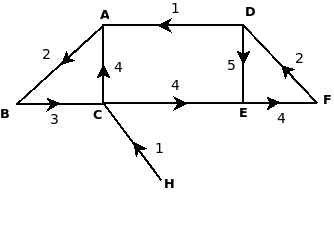
\includegraphics[scale=0.6]{Fig2_4_a1.png}\\
      \hspace*{1.5in}\textbf{$G_0$}\\
      
      $C_1 = \{(C,A),(A,B),(B,C)\}\\
      BV = \{A,B,C\}\\
      BA = \{(C,A),(A,B)\}$ \\
    }\hfill\\
  \parbox{6cm}
  {
    \hspace*{-.5in}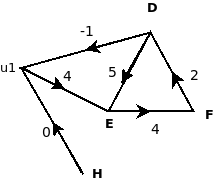
\includegraphics[scale=0.6]{Fig2_4_a2.png}\\
    \hspace*{.25in}\textbf{$G_1$}\\
    
    $C_2 = \{(F,D), (D,E), (E,F)\}\\
    BV = \{D,E,F\}\\
    BA = \{(F,D),(D,E)\}$ \\
  }\hfill
  \parbox{6cm}
  {
    \hspace*{-.5in}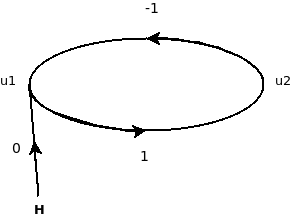
\includegraphics[scale=.6]{Fig2_4_a3.png}\\
    \hspace*{.5in} \textbf{$G_2$}\\
    
    $BV = \{H,u_1,u_2\} = V_2 \\
    BA = \{(u_1,u_2)\} = max. ramificaci\acute{o}n$\\
}\hfill\\
\parbox{10cm}
{
  \textbf{(b)} Reconstrucción de $G_{k-1}, G_{k-2}, \ldots, G_0$\\
  La máxima ramificación tiene peso 17.\\

  $G_2: BA = \{(u_1,u_2)\} \rightarrow G_1: \\ BA = \{(u_1,E),(E,F),(F,D)\} \rightarrow G_0: \\ BA = \{(C,E),(E,F),(F,D),(C,A),(B,C)\} $
}\hfill\\
\hrule


\subsection{Enumeración de árboles de expansión}

En general, un grafo tiene un número de árboles de expansión distintos. Para algunas aplicaciones es útil para construir árboles de expansión con cualidades específicas. Sin embargo, no se trata aquí de sus cualidades individuales, sino más bien, con el número total de árboles asociados de un grafo determinado.

Antes de resolver el problema general sería conveniente conocer el resultado específico obtenido por Cayley\cite{c}

\begin{teorema}
El número de árboles de expansión de $K_n$ es $n^{n-2}$.
\end{teorema}
\begin{proof}
El número total de árboles de expansión de $K_n$ es evidentemente el mismo que el número de árboles que se puede construir en $n$ distinguido, es decir, con vértices etiquetados. Sea $T$ un árbol en el que los vértices están etiquetados $1,2, \ldots, n$.

\begin{figure}[H]
\caption{ }
\end{figure}
\hrulefill{}\\
\parbox{6cm}
{
\hspace*{.5in}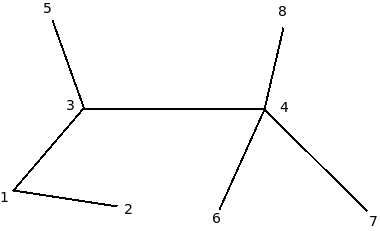
\includegraphics[scale=.55]{Fig2_5.png}
}\hfill\\
\hrule

Podemos generar una secuencia de $(n-2)$ etiquetas, $S$, únicamente codifica $T$ de la siguiente manera. Al elegir el $i$-ésimo elemento de $S$ se elimina el vértice de un grado de $T$ que tenga la menor etiqueta. El $i$-ésimo elemento es entonces la etiqueta de los vértices restantes en $T$, que se encontrab junto al vértice eliminado. El proceso se detiene cuando sólo quedan dos vértices en $T$.

Por el contrario, podemos construir un único árbol, con $n$ vértices de una secuencia $S$, de $(n-2)$ etiquetas de la siguiente manera. Sea $I$ la lista de etiquetas ($1,2, \ldots,n$). En primer lugar, buscamos la etiquet más pequeña en $I$ que no esté en $S$. Sea esta $i_1$. La arista $(i_1,s_1)$ se encuentra entonces en $T$. Quitamos $i_1$ de $I$ y $s_1$ de $S$ y repetimos el proceso con un nuevo $S$ e $I$. Por último, $S$ no contiene elementos y la última arista en incorporarse a $T$ es la definida por el par restante de las etiquetas en $I$.

Así pues, es una correspondencia uno-a-uno entre los árboles de expansión de $K_n$ y las palabras de longitud $(n-2)$ sobre el alfabeto $(1,2, \ldots,n)$. El número de esas palabras es $n^{n-2}$ y por lo tanto el teorema continua de la siguiente manera.
\end{proof}

Llegamos ahora al problema general de contar el número de árboles de expansión para un uso arbitrario multi-grafo de $G$. Esto requiere que primero se concentren en dígrafos y contando el número de árboles de expansión cuya raíz sea un vértice particular. A tal fin, introducimos ahora el llamado \emph{Kirchoff} o una matriz de grados $K(G)$. Los elementos de $K$ se definen como sigue:

\begin{align}
K(i,j) & = g^-(v_i), i = j \nonumber \\
& = -k, i \ne j \nonumber
\end{align}

donde $k$ es el número de aristas de $i$ a $j$. Dentro de esta definición el grafo se presume que no tiene bucles. Si existiera en un grafo de interés, entonces pueden ser borrados con seguridad porque no pueden contribuir al número de árboles de expansión. Figura 2.6 (a).

Observe que la suma de las entradas de cualquier columna de $K$ es necesariamente igual a cero. Podemos usar $K$ para identificar al conjunto $\{g_i\}$ de subgrafos de $G$, en el que cada vértice $v$ tiene $g^-(v) = 1$, siempre que $G$, $g^-(v) \ge 1$. El procedimiento  se entiende mejor con la ayuda de un ejemplo. En la figura 2.6 (b) el determinante de $K$, para el grafo de la figura 2.6 (a) se extiende a una suma de determinantes, para cada correspondiente $g_i$. Este procedimiento es siempre posible por una aplicación continua de la identidad:

\[ det(c_1,c_2, \ldots,(c_j + c^{'}_j), \ldots, c_n) = \]
\[ det(c_1, c_2, \ldots, c_j, \ldots, c_n) + det(c_1,c_2, \ldots, c^{'}_j, \ldots, c_n) \]

donde cada $c_i$ es un columna de $n$ elementos. Las aplicaciones siguientes se utilizan para reducir el valor de un elemento de la diagonal que es mayor que uno y para producir dos determinantes, cada uno con la suma de los elementos en cualquier columna igual a cero. La expansión se detiene cuando cada elemento de la diagonal de los determinantes creados no son superiores a uno. Tenemos entonces

\[ det(K(G)) = \sum_i det(K(g_i)) \]

donde $K(g_i)$ es el grado de la matriz de $g_i$. En nuestro ejemplo, $g_i$ es elaborado por a través de su determinante asociado $det(K(g_i))$ en la figura 2.6 (b).

\begin{figure}[H]
\caption{ }
\end{figure}
\hrulefill{}\\
\parbox{3cm}
{
  \textbf{(a)}\\
  \hspace*{.5in}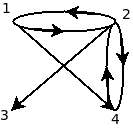
\includegraphics[scale=.5]{Fig2_6_a1.png}
}\hspace*{.5in}
\parbox{2cm}
{
  \[
  K = \left[ \begin{array}{lccl}
      1 &  -1 &  0 &  -1 \\
      -1 &  2  & -1 & -1 \\
      0 &  0 &  1  & 0 \\
      0 &  -1 &  0  & 2 
    \end{array}
  \right]
  \]
}\hfill\\
\hrule
\hspace*{-1.2in}\parbox{6cm}
{
  \textbf{(b)}\\
    \[
    det(K) = \left| \begin{array}{cccc}
        1 & 0 & 0 & 0 \\
        -1 & 1 & -1 & 1 \\
        0 & 0 & 1 & 0 \\
        0 & -1 & 0 & 1
      \end{array}
    \right| \quad+ \]
 \hspace*{.8in}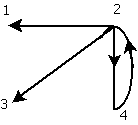
\includegraphics[scale=.6]{Fig2_6_b1.png}
 \begin{center} $\textcolor{rojo}{\uparrow} g_1$ \end{center}
}\hfill
\parbox{6cm}
{
  \[
   \left| \begin{array}{cccc}
        1 & 0 & 0 & -1 \\
        -1 & 1 & -1 & 0 \\
        0 & 0 & 1 & 0 \\
        0 & -1 & 0 & 1 
      \end{array}
    \right| \quad +\]
    \hspace*{.7in}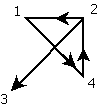
\includegraphics[scale=.65]{Fig2_6_b2.png}
    \begin{center} $\textcolor{rojo}{\uparrow} g_2$ \end{center}
}\hfill\\
\parbox{6cm}
{
    \[
    \left| \begin{array}{cccc}
        1 & -1 & 0 & 0 \\
        -1 & 1 & -1 & -1 \\
        0 & 0 & 1 & 0 \\
        0 & 0 & 0 & 1 
      \end{array}
    \right| \quad +\]
    \hspace*{.3in}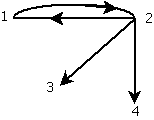
\includegraphics[scale=.6]{Fig2_6_b3.png}
    \begin{center} $\textcolor{rojo}{\uparrow} g_3$ \end{center}
}
\hspace*{-.5in}\parbox{6cm}
{
    \[
    \left| \begin{array}{cccc}
        1 & -1 & 0 & -1 \\
        -1 & 1 & -1 & 0 \\
        0 & 0 & 1 & 0 \\
        0 & 0 & 0 & 1 
      \end{array}
    \right| \]
    \hspace*{.3in}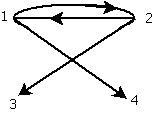
\includegraphics[scale=.6]{Fig2_6_b4.png}
    \begin{center} $\textcolor{rojo}{\uparrow} g_4$ \end{center}
}\hfill\\
\hrule
\hspace*{-1in}\parbox{6cm}
{
  \textbf{(c)}\\
  \[
  det (K(G_2)) = \left | \begin{array}{cccc}
      1 & 0 & 0 & -1 \\
      -1 & 0 & -1 & 0 \\
      0 & 0 & 1 & 0 \\
      0 & 0 & 0 & 1 \\
      \end{array}
      \right | \quad + \]
      \hspace*{1in}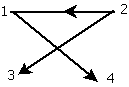
\includegraphics[scale=.65]{Fig2_6_c1.png}
      \begin{center} $\textcolor{rojo}{\uparrow} g_1$ \end{center}
}
\parbox{6cm}
{
  \vspace*{.5in}
  \[
  \left | \begin{array}{cccc}
      1 & 0 & 0 & 0 \\
      -1 & 0 & -1 & -1 \\
      0 & 0 & 1 & 0 \\
      0 & 0 & 0 & 1 \\
    \end{array}
  \right | \]
  \hspace*{.5in}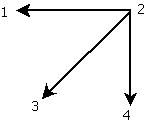
\includegraphics[scale=.65]{Fig2_6_c2.png}
  \begin{center} $\textcolor{rojo}{\uparrow} g_2$ \end{center}

}\nopagebreak\vfill
\hspace*{-1.1in}\parbox{6cm}
{
  \[
  det (K(G_3)) = \left | \begin{array}{cccc}
      1 & 0 & 0 & 0 \\
      -1 & 1 & 0 & -1 \\
      0 & 0 & 0 & 0 \\
      0 & -1 & 0 & 1 \\
    \end{array}
  \right | \quad + \]
  \hspace*{1in}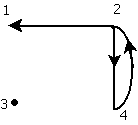
\includegraphics[scale=.65]{Fig2_6_c3.png}
  \begin{center} $\textcolor{rojo}{\uparrow} g_1$ \end{center}
}
\hspace*{-.3in}\parbox{6cm}
{
  \[
  \left | \begin{array}{cccc}
      1 & 0 & 0 & -1 \\
      -1 & 1 & 0 & 0 \\
      0 & 0 & 0 & 0 \\
      0 & -1 & 0 & 1 
      \end{array}
    \right |\quad+ \]
    \hspace*{.85in}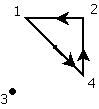
\includegraphics[scale=.675]{Fig2_6_c4.png}
    \begin{center} $\textcolor{rojo}{\uparrow} g_2$ \end{center}
}\vfill
\hspace*{-.7in}\vspace*{.3in}\parbox{6cm}
{
  \[
  \left | \begin{array}{cccc}
      1 & -1 & 0 & 0 \\
      -1 & 1 & 0 & -1 \\
      0 & 0 & 0 & 0 \\
      0 & 0 & 0 & 1 
      \end{array}
    \right | \quad + \]
    \hspace*{.4in}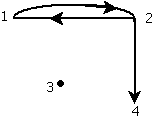
\includegraphics[scale=.65]{Fig2_6_c5.png}
    \begin{center} $\textcolor{rojo}{\uparrow} g_3$ \end{center}
}
\parbox{1cm}
{
  \[
  \left | \begin{array}{cccc}
      1 & -1 & 0 & -1 \\
      -1 & 1 & 0 & 0 \\
      0 & 0 & 0 & 0 \\
      0 & 0 & 0 & 1 
      \end{array}
    \right | \]
    \hspace*{.2in}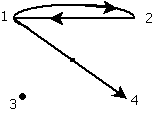
\includegraphics[scale=.65]{Fig2_6_c6.png}
    \begin{center} $\textcolor{rojo}{\uparrow} g_4$ \end{center}
}\hrule
\hfill
\nopagebreak
En la expansión de la figura 2.6 (b) cada $g_i$ corresponde a un subgrafo de $G$ en el que $g^-(v) = 1$, si en $G$, $g^-(v) \ge 1$. Evidentemente, cada subgrafo de $G$ se representa precisamente una vez en esta expansión. Consideremos la expansión de la raíz de un árbol como un vértice particular $v$ de $G$ y sea $T$ tal que un árbol. Si $g^-(r) > 1$, entonces $T$ aparece exactamente en $g^-(v)$ de $g_i$. Cada uno de estos $g_i$ comienza en $T$ más una posible arista incidente a $r$. Pero, sin embargo, si $g^-(v) = 0$ ó $1$ entonces $T$ aparece en uno de $g_i$ únicamente. Si dejamos que $G_r$ denote $G$ con aquellas aristas incidentes a $r$ que han sido eliminadas, entonces podemos ampliar $det(K(G_r))$ de acuerdo con el método previsto anteriormente. En esta expansión, sin embargo, cualquier árbol raíz de $r$ estará representado por un término exacto. En la figura 2.6 (c) podemos ver dos ejemplos. Observe que cada término de estas ampliaciones es el determinante del grado de una matriz para un subgrafo $g'_i$ de $G$ donde $g^-(v) \le 1, v \ne r$, y $g^-(r) = 0$.

Ahora necesitamos el siguiente teorema en el que $det(K_{rr}(G))$ denota el menor resultado de eliminar la $r$-ésima columna y la $r$-ésima fila de $det(K_{rr}(G))$.

\begin{teorema}
Si $g$ es un dígrafo finito tal que para cada vértice $v$, $g^-(v) \le 1$, entonces
\begin{align}
det (K_{rr}(g)) & = 1\ si\ g\ contiene\ un\ \acute{a}rbol\ ra\acute{\dotlessi}z\ de\ expansi\acute{o}n\ r \nonumber\\
& = 0\ en\ otro\ caso\ \nonumber
\end{align}
\end{teorema}
\begin{proof}
Supongamos que $g$ contiene un árbol de expansión $T$ enraizado en $r$, y que sus vértices están etiquetados $1,2,\ldots,n$. Entonces $g = T$ o $g = T + a$ donde $a$ es una arista incidente a $r$. Podemos renombrar los vértices de acuerdo con una amplitud de primer orden al atravesar $T$, visitando primeramente $r$. Entonces $r = 1$, de modo que $K(1,1) \le 1$ y para $i > 1$, $K(i,i) = 1$. Además, si $i \ne 1$ y $i > j$ entonces $K(i,j) = 0$. Así, $K_{11}(g)$ es la parte de una matriz triangular superior con elementos unitarios en la diagonal, y así $det(K_{11}(g)) = 1$.

Ahora bien, supongamos que $g$ no contiene un árbol de expansión enraizado en $r$. Si cualquier vértice $v \ne r$ tiene $g^-(v) = 0$, entonces la columna correspondiente de $K$ consta sólo de ceros, de modo que $det(K_{rr}(g)) = 0$. Supongamos entonces que cada vértice $v \ne r$ tiene $g^-(v) = 1$. Como $g$ no contiene un árbol enraizado en $r$, entonces debe contener un circuito que excluya $r$ de la siguiente manera. Trazar una arista donde $v_i \ne r$ hacia atrás hasta $v_j$ y una arista desde $v_j$ retrocediendo hasta $v_k$ y así sucesivamente. Si $r$ es finalmente alcanzado en este proceso, entonces $v_i,v_j,v_k,\ldots$ pertenecen a un subárbol en $r$. En caso contrario, el proceso termina trazando un circuito no incluido en $r$. Si se alcanza $r$ repetiremos el proceso inicial con los vértices que no están en el subárbol. Consideremos ahora el conjunto de columnas de $K$ correspondiente a los vértices de un circuito. Cualquier fila de este conjunto contiene sólo ceros o que contiene un solo ($-1$) y un solo ($+1$). Así, la suma de ests columnas es una columna de ceros. De ello se deduce que $det(K_{rr}(g)) = 0$.
\end{proof}

El $g'_i$ (y de paso $g_i$) se definió anteriormente para satisfacer el teorema 2.4. Hay que tener en cuenta que $K_{rr}(G)$ es idéntico a $K(G_r)$, salvo que el ($rr$)-ésimo elemento sea la unidad en vez de cero. Es evidente que hay una correspondencia uno-a-uno entre los términos de $det(K_{rr}(G))$ y de $det(K(G_r))$ si cada uno se ha ampliado de acuerdo a la prescripción dada anteriormente. En efecto:

\[det\ (K_{rr}(G))\ = \sum_{i}\ det\ (K_{rr}(g'_{i}))\]

y si aplicamos el teorema 2.4 por encima a cada término de la suma obtendremos inmediatamente el siguiente teorema.

\begin{teorema}
El número de árboles de expansión de raíces $r$ en un grafo finito $G$ es igual a $det(K_{rr}(G))$.
\end{teorema}

La Figura 2.7 ilustra un algoritmo eficiente, basado en el teorema 2.5 para calcular el número de árboles de expansión de raíz $r$. Ahora bien, $K$ es una matriz $n \times n$ de Kirchoff y la línea 1 del algoritmo asigna (o introduce) los elementos de $K_{rr}$ en una matriz determinante $A$ de $(n-1) \times (n-1)$. Esto claramente se puede hacer en $O(n^2)$ pasos. Las líneas 2-5 usan el método de Gauss para convertir A en una matriz triangular superior. En otras palabras, una serie de sustracciones de filas reducen cada elemento $A(i,j)$ de $A$, para los que $i > j$, a cero. Esto se logra en $O(n^3)$ pasos. El determinante es entonces evaluado por la diagonal ampliada en las líneas 7-8 usando $O(n)$ pasos, donde el resultado se almacenará en $DKRR$.
\vfill
\begin{algorithm}[H]
\caption{Un Algoritmo para encontrar el número de árboles de expansión de raíces r en un dígrafo con matriz de grado K, o el número de árboles de expansión de un grafo no dirigido con matriz de grado K}
\BlankLine
\dontprintsemicolon
$A \leftarrow K_{rr}$\;
\For{$k = 2${\KwTo} $(n-1)$}
{
  \For{$i = k${\KwTo} $(n-1)$}
  {
    \For{$j = 1${\KwTo} $(n-1)$}
    {
      $A(i,j) \leftarrow A(i,j) - (A(i,(k-1))/A((k-1))).A((k-1),j)$\;
    }
  }
}
$DKRR \leftarrow A(1,1)$\;
\For{$i=2${\KwTo} $(n-1)$}
{
  $DKRR \leftarrow DKRR.A(i,i)$
}
\end{algorithm}

Habiendo resuelto el problema de contar el número de árboles de expansión de raíces en un vértice dado en un dígrafo, podemos ver muy rápidamente una solución al problema de contar los árboles de expansión de un grafo no dirigido. Para ello sabiendo que, dado un grafo no dirigido $G$, podemos construir un dígrafo $G'$ reemplazando cada arista $(u,v)$ por dos aristas dirigidas $(u,v)$ y $(v,u)$. Luego, por cada árbol de expansión de $G$ corresponderá un árbol de expansión $G'$ de raíces en un vértice particular, y viceversa. Se define la matriz de grado $G$ para que sea idéntica a la matriz de grado $G'$, que se denota también por $K$.

\begin{teorema}
El número de árboles de expansión en un grafo no dirigido finito es igual a cualquiera de los $det(K_{rr}(G))$ para $1\le r \le n$.
\end{teorema}

El teorema contempla la solución obvia de que el número de árboles de expansión no puede depender de la elección de $r$. Como el título de la Figura 2.7 implica, obviamente podremos utilizar ese algoritmo de $O(n^3)$ para contar el número de árboles de expansión de un grafo no dirigido, así como para contar árboles de expansión de raíces en un vértice particular de un dígrafo.

\section{Circuitos, conjuntos de corte y conectividad}
En esta sección demostraremos la importancia de los árboles de expansion con respecto al espacio del circuito y al llamado conjunto de corte de un grafo.

Sería conveniente aquí ampliar nuestras definiciones. Un \emph{co-árbol} es un grafo $G = (V,A)$ con respecto a un árbol de expansión $T = (V,A')$ que es el conjunto de aristas $(A-A')$. Si $G$ tiene $n$ vértices entonces cualquier co-árbol, si existe, tendrá $|A| - (n-1)$ aristas. Cualquier arista de un co-árbol es llamada como \emph{cuerda} de un árbol de expansión. También tenemos que definir la operación del \emph{anillo de suma}. El \emph{anillo de suma} de dos grafos $G_1 = (V_1,A_1)$ y $G_2 = (V_2,A_2)$, que escribimos como $G_1 \oplus G_2$, es el grafo $((V_1 \cup V_2)), ((A_1 \cup A_2)) - (A_1 \cap A_2))$. En otras palabras el conjunto de aristas de $G_1 \oplus G_2$ consiste en que las aristas que se encuentren en $G_1$ o en $G_2$ pero que no están en ambos. Es fácil ver que la operación del anillo de suma es tanto conmutativa como asociativa. Es decir, que:
\[ G_1 \oplus G_2 = G_2 \oplus G_1\]
y que
\[(G_1 \oplus G_2) \oplus G_3 = G_1 \oplus (G_2 \oplus G_3)\]

\subsection{Circuitos fundamentales de un grafo}
Del teorema 1.2 vemos que la adición de un acorde a un árbol de expansión de un grafo crea precisamente un circuito. En un grafo de la colección de estos circuitos con respecto a un árbol de expansión particular, se le llama conjunto de \emph{circuitos fundamentales}. Como veremos, ninguno de los circuitos arbitrarios del grafo se pueden expresar como una combinación lineal de los circuitos fundamentales mediante la operación del anillo de suma. En otras palabras, los circuitos fundamentales forman una \emph{base} para el espacio del circuito.

\begin{figure}[H]
\caption{Algunos circuitos de $G$ expresados como una combinación lineal de circuitos fundamentales de $G$ con respecto a $T$}
\end{figure}
\hrulefill{}\\
\parbox{6cm}
{
  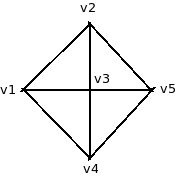
\includegraphics[scale=.5]{Fig2_8_1.png}\\
  \hspace*{.5in}$G$
}
\hspace*{-.2in}\parbox{6cm}
{
  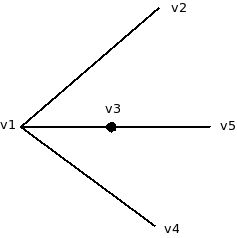
\includegraphics[scale=.6]{Fig2_8_2.png}\\
  $T$: árbol de expansión de $G$.
}\hfill
\hspace*{-.5in}\parbox{10cm}
{
  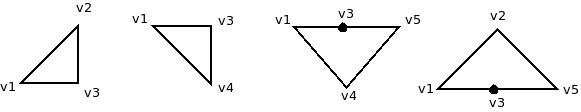
\includegraphics[scale=.6]{Fig2_8_3.png}\\
 \hspace*{.25in} El conjunto fundamental de circuitos de $G$ con respecto a $T$.
}\hfill\\
\hspace*{-.3in}\parbox{3cm}
{
\includegraphics[scale=.6]{Fig2_8_4.png} 
}
\parbox{1cm}
{
$=$}
\parbox{3cm}
{
\includegraphics[scale=.6]{Fig2_8_5.png}
}
\hspace*{.1in}\parbox{1cm}
{
$\oplus$
}
\parbox{3cm}
{
\includegraphics[scale=.6]{Fig2_8_6.png}
}\hfill\\
\hspace*{-.5in}\parbox{3cm}
{
\includegraphics[scale=.6]{Fig2_8_7.png} 
}
\parbox{1cm}
{
$=$}
\parbox{3cm}
{
\includegraphics[scale=.6]{Fig2_8_8.png}
}
\hspace*{.1in}\parbox{1cm}
{
$\oplus$
}
\parbox{3cm}
{
\includegraphics[scale=.6]{Fig2_8_9.png}
}\hfill\\
\hspace*{-.9in}\parbox{2cm}
{
\includegraphics[scale=.6]{Fig2_8_10.png} 
}
\parbox{2cm}
{
\hspace*{.45in}$=$
}
\parbox{2cm}
{
\includegraphics[scale=.6]{Fig2_8_11.png}
}
\hspace*{.1in}\parbox{1cm}
{
$\oplus$
}
\parbox{2cm}
{
\includegraphics[scale=.6]{Fig2_8_12.png}
}
\parbox{1cm}
{
$\oplus$
}
\hspace*{-.25in}\parbox{2cm}
{
\includegraphics[scale=.6]{Fig2_8_13.png}
}\hrule
\hfill
\nopagebreak

La figura 2.8 muestra, para el grafo ilustrado hay, un árbol de expansión $T$, el conjunto correspondiente de los circuitos fundamentales y algunos otros circuitos expresados como combinaciones lineales de estos. En general, entonces, tenemos el siguiente teorema.

\begin{teorema}
Un conjunto de circuitos fundamentales, con respecto a algún árbol de expansión de un grafo $G$, constituye una base del espacio del
circuito de $G$.
\end{teorema}
\begin{proof}
En primer lugar, hay que tener en cuenta cualquiera de los circuitos se puede expresar como una combinación lineal de los circuitos de $F$ con respecto a algún árbol de expansión $T$. Denotamos un circuito $C$ arbitrario por su conjunto de aristas:
\[ C = {a_1, a_2, \ldots, a_i, a_{i+1}, \ldots, a_j}\]
donde $a_k$ para $1 \le k \le i$ es una cuerda de $T$ y para $i < k \le j$ es una arista de $T$. $F$ contiene precisamente un circuito fundamental que contiene a cada $a_k$ para $1 \le k \le i$. Denotamos al circuito fundamental que contiene $a_k$ por $C(a_k)$. Definimos ahora como $C'$ del siguiente modo:
\[ C' = C(a_1) \oplus C(a_2) \oplus \ldots \oplus C(a_k) \]
y mostramos así como $C$ y $C'$ contiene precisamente al mismo conjunto de aristas. Si no lo hacen entonces:
\[ C \oplus C' \ne \emptyset \]
Para cualesquiera dos circuitos $C_1$ y $C_2$, $C_1 \oplus C_2$ debe ser un circuito o una unión disjunta de aristas de circuitos. Así $C'$ es un circuito o una unión disjunta de aristas de circuitos y es tal que $C \oplus C'$. Sin embargo, $C$ y $C'$ solo contienen el conjunto de cuerdas $a_1, a_2, \ldots, a_k$ de $T$ y no otras cuerdas. Así, $C \oplus C'$ sólo puede tener aristas de $T$ y aquellas que no contengan un circuito. Por lo tanto tenemos una contradicción en donde nuestra hipótesis $C \ne C'$ debe ser errónea.

Completamos la demostración al señalar que ningún miembro de $F$ se puede expresar como un anillo de suma lineal de los otros circuitos de $F$. Esto se deduce inmediatamente de la observación de que cada cuerda de $T$ está contenida en uno y sólo un circuito fundamental.
\end{proof}

Tenemos un corolario inmediato:
\begin{cor}
El espacio del circuito para un grafo con $|A|$ aristas y $n$ vértices tiene dimension $(|A| - n + 1)$.
\end{cor}

Un conjunto de circuitos fundamentales, \emph{FCS (Fundamental Circuit Set)}, de un grafo $G$ se puede encontrar fácilmente en tiempo polinómico. El algoritmo descrito en la figura 2.9, por ejemplo, opera en tiempo $O(n^3)$. La línea 1 establece que un árbol de expansión $T$ y su correspondiente co-árbol $CT$ de $G$ se encontraron en primera instancia. Como vimos en el capítulo 1 un árbol de expansión se puede encontrar en un tiempo $O(max\ (n,|A|))$. Es fácil modificar el algoritmo, tal que cuando se encuentre una arista que no sea requerida para $T$, esta no sea descartada para ser añadida a $CT$. Es más, esto fácilmente se puede hacer sin costo alguno para el orden de complejidad. Así la línea 1 se puede lograr en tiempo $O(max\ (n,|A|))$.

Para cada arista de $a_i \in CT$ del cuerpo de la declaración en la líneas 4-6 se encuentra un circuito fundamental y lo agrega al conjunto $FCS$. La búsqueda de la ruta en $T$ la cual genera un circuito con $a_i$ en la línea 4 puede lograrse en $O(n)$ pasos tal como sigue. El vértice $v_i$ en $T$ es etiquetado como uno. Entonces a partir de $v_i$ y empleando primeramente un recorrido en anchura de $T$, cada vértice $v$ se denomina $(L+1)$ donde $L$ es la etiqueta del padre de $v$. El proceso se detiene cuando $v'_1$ adquiere una etiqueta. El camino desde $v'_1$ hacia $v_i$ es entonces fácilmente trazable si empezamos en $v'_1$ y procedemos así en cada paso con el siguiente vértice visitado colocandole una etiqueta que es numéricamente una menos que la del vértice actual. En este subalgoritmo el etiquetado inicial claramente se puede lograr en $O(n)$ pasos. El tiempo total dedicado al recorrer las aristas en los vértices al trazar la ruta de acceso es $O(n)$, en el peor de los casos cada arista se recorre dos veces a excepción de las aristas inicial y final y $T$ contiene $(n-1)$ aristas. El camino a lo sumo es la acumulación de las $(n-1)$ aristas y así todo el camino para encontrar el proceso no requiere más de tiempo $O(n)$.
\nopagebreak
\begin{algorithm}[H]
\caption{ }
\BlankLine
\dontprintsemicolon
Encontrar un árbol de expansión $T$ y el correspondiente co-árbol $CT$ de $G$\;
$FCS \leftarrow \emptyset$\;
\For{todo $a_i = (v_i,v'_i) \in CT$}
{
  \Begin{
    encontrar el camino desde $v_i$ hasta $v'_i$ en $T$ y denotemoslo por $P_i$\;
    $C_i \leftarrow P_i \cup {a_i}$\;
    $FCS \leftarrow FCS \cup C_i$\;
  }
}
\end{algorithm}


El número de aristas en $CT$ es $O(|A|)$, es decir, $O(n^2)$ con carácter general o $O(n)$ para un grafo disperso. Así, el cuerpo de la sentencia for se ejecuta en un tiempo $O(|A|)$ en las líneas 3-6, que en esencia determinan la complejidad general del algoritmo, que puede ser ejecutado en tiempo $O(n^2)$ para un grafo disperso, y en el peor de los casos, en tiempo $O(n^3)$.

\subsection{Conjuntos de corte fundamentales de un grafo}

Un conjunto de corte de un grafo conexo, o una componente, es un conjunto de aristas cuya eliminación desconecta al grafo o a la componente. Como parte de la definición no será el subconjunto propio el que cause la desconexión. Una consecuencia de esto es que uno de los conjuntos de corte produce exactamente dos componentes.

A veces es útil para indicar un conjunto límite fijado por la partición de los vértices que induce. Si $V$ denota el conjunto de vértices de $G$ y si $P$ es el subconjunto de vértices en una componente de $G$ inducida por el conjunto de corte, entonces el límite del conjunto se puede especificar por $(P,\bar{P})$ donde $\bar{P} = V - P$.

Sea $T$ un árbol de expansión del grafo $G$. Cualquier arista de $T$ define una partición de los vértices de $G$ desde que su traslado desconecta a $T$ en dos componentes. Habrá por tanto un conjunto de corte correspondiente de $G$ que producirá la misma partición de los vértices. Este conjunto de corte contiene precisamente una de las aristas y un número de cuerdas de $T$. Así que este conjunto de corte se le llama \emph{conjunto de corte fundamental} de $G$ con respecto a $T$.

\begin{figure}[H]
\caption{ }
\end{figure}
\hrulefill{}\\
\parbox{6cm}
{
  \includegraphics[scale=.6]{Fig2_10_1.png}\\
  $G$
}
\parbox{8cm}
{
  \includegraphics[scale=.61]{Fig2_10_2.png}\\
  \hspace*{-.2in}$T$: un árbol de expansión de $G$.
}\hfill\\
\parbox{10cm}
{
  \begin{align}
    C_1 = \{a_1, a_2, a_5, a_8\} \nonumber\\
    C_2 = \{a_4, a_2, a_5, a_7\}\nonumber \\
    C_3 = \{a_6, a_7, a_8\} \nonumber\\
    C_4 = \{a_3, a_5, a_8\} \nonumber
  \end{align}
  El conjunto fundamental de conjuntos de corte de $G$ con respecto a $T$.\\
  \begin{align}
    \{a_3 , a_5, a_6, a_7\} = C_3 \oplus C_4 \nonumber\\
    \{a_1, a_4, a_6\} = C_1 \oplus C_2 \oplus C_3 \nonumber\\
    \{a_1, a_2, a_5, a_8\} = C_1 \oplus C_2 \oplus C_3 \oplus C_4 \nonumber
  \end{align}
}\hrule
\hfill

Algunos conjuntos de corte de $G$ se expresan como combinaciones lineales de los conjuntos fundamentales de corte de $G$ con respecto a $T$.

\begin{teorema}
El conjunto de corte fundamental con respecto a algún árbol de expansión forma una base para el conjunto de corte de un grafo.
\end{teorema}

\begin{proof}
Esto es totalmente análogo al del teorema 2.7 y por ello se omiten detalles. La función principal de la demostración, tomando un conjunto de corte arbitrario de $CS$:
\[ CS = a_1, a_2, \ldots, a_i, a_{i+1}, \ldots, a_j\]
donde $a_k$ para $1 \le k \le i$ son aristas del árbol de expansión y $a_k$ para $i < k \le j$ son cuerdas, se muestra que $CS$ es identico a $CS'$:
\[ CS' = CS(a_1) \oplus CS(a_2) \oplus \ldots \oplus CS(a_i) \]
donde $CS(a)$ es el conjunto de corte fundamental asociado con una arista $a$ de $T$.\\

Podemos ver esto de la siguiente manera informal. Sea $C_1 = (V_1,\bar{V}_1)$ y $C_2 = (V_2,\bar{V}_2)$ un conjunto de corte de un grafo $G$. Si las aristas de ambos conjuntos $C_1$ y $C_2$ son retirados de $G$, entonces los vértices se dividen en cuatro subconjuntos $(V_1 \cap V_2), (V_1 \cap \bar{V}_2) (\bar{V}_1 \cap V_2)$ y $(\bar{V}_1 \cap \bar{V}_2)$ tales que ninguna arista de G conecta los restantes vértices en diferentes subconjuntos. La suma del anillo de $C_1$ y $C_2$ se compone de las aristas en $C_1$ y $C_2$ pero no de aquellas que se encuentren tanto en $C_1$ como en $C_2$. Las aristas comunes a ambos $C_1$ y $C_2$ sólo pueden conectar vértices de $(V_1 \cap V_2)$ hacia los vértices de $(\bar{V}_1 \cap \bar{V}_2)$ o que esten en $(\bar{V}_1 \cap V_2)$ hacia vértices de $(\bar{V} \cap V_2)$. Así, si las aristas de $C_1 \oplus C_2$ se eliminan de $G$ se formarán una partición de vértices dentro de cada subconjunto $(V_1 \cap V_2) \cup (\bar{V}_1 \cap \bar{V}_2)$ y $(V_1 \cap \bar{V}_2) \cup (\bar{V}_1 \cap V_2)$. Si cada uno de estos subconjuntos induce un subgrafo conexo entonces $C_1 \oplus C_2$ es un conjunto de corte. De lo contrario, será una unión disjunta de aristas del conjunto de corte.
\end{proof}

\begin{figure}[H]
\caption{Para ilustrar, con referencia a la figura 2.10, que el anillo de la suma de dos conjuntos de corte arbitrarios o la unión disjunta de aristas del conjunto de corte}
\hrulefill{}\\
\end{figure}
\parbox{10cm}{
\begin{align}
\{a_1, a_4, a_6\} \oplus \{a_2, a_3, a_4, a_6\} & = \{a_1, a_2, a_3\} \nonumber\\
\{a_4, a_1, a_7, a_8\} \oplus \{a_3, a_5, a_6, a_7\} & = \{a_1, a_3, a_4, a_5, a_6, a_8\} \nonumber\\
& = \{a_1, a_4, a_6\} \cup \{a_3, a_5, a_8\} \nonumber
\end{align}}\hrule
\hfill

\begin{cor}
El espacio del conjunto de corte establecido para un grafo con $n$ vértices tiene dimensión $(n-1)$.
\end{cor}

En cuanto al caso de los circuitos fundamentales, es fácil construir un algoritmo de tiempo polinómico para encontrar un conjunto de corte fundamental.

\subsection{Conectividad}

Los circuitos y los conjuntos de corte son aspectos de la conexión de un grafo.

Es evidente que la eliminación de cualquier vértice de un árbol lo desconecte. Por otro lado, la eliminación de cualquier vértice o subconjunto de vértices de un grafo completo no lo desconecta. Los árboles y grafos completos representan los dos casos extremos de \emph{conectividad de vértices}, o simplemente \emph{conectividad} de un grafo. Para un grafo arbitrario $G$, definimios su conectividad, escribiendo $K_v(G)$ o simplemente $K_v$, siendo esto el número mínimo de vértices cuya eliminación hará no conexo a $G$. También se dice que $G$ es \emph{h-conexo} para cualquier valor entero positivo $h$ que satisfaga que $h \le K_v(G)$. Cualquier subconjunto de vértices cuya eliminación desconecte al grafo $G$ se le llamará \emph{vértice de corte}.

Del mismo modo se define la \emph{arista de conectividad}, $K_a(G)$ o $K_a$, para el grafo conexo $G$ donde es el tamaño de los más pequeños conjuntos de corte de $G$. $G$ se dice que es \emph{arista-h-conectado} para cualquier valor entero positivo $h$ que satisfaga $h \le K_a(G)$.

Denotamos el menor grado de cualquier vértice en un grafo por $\delta$. Dado que el conjunto de aristas incidentes con cualquier vértice forma un conjunto de corte, se tiene que $\delta \ge K_a(G)$. También $K_v(G)$ no puede superar a $K_a(G)$. Podemos ver esto de manera informal mediante el reconocimiento de que un vértice de corte se puede obtener mediante la eliminación de un extremo de cada arista de un conjunto de corte minimal. Por conveniencia se define $K_v(K_n)$ para ser $(n-1)$. Entonces tenemos el siguiente teorema:

\begin{teorema}
Para cualquier grafo conexo $G$:
\[ K_v(G) \le K_a(G) \le \delta \]
\end{teorema}

Describimos ahora un teorema para grafos bi-conexos antes de afirmar su generalización para grafos h-conexos.

\begin{teorema}
Un grafo $G$ con al menos tres vértices es un bloque si y sólo si dos vértices están conectados por al menos dos caminos de aristas disjuntas.
\end{teorema}
\begin{proof}
Si cualquiera de los dos vértices de $G$ están conectados por al menos dos caminos de aristas disjuntas entonces $G$ es conexo y no puede contener un punto de articulación. Por lo tanto $G$ debe ser un bloque.

Por otra parte, supongamos que $G$ es bi-conexo. Sea $l(u,v)$ la longitud del camino de $u$ a $v$. Se prueba, por inducción sobre $l(u,v)$ que hay dos caminos de aristas disjuntas desde $u$ a $v$. Si $l(u,v) = 1$, entonces $(u,v)$ no puede ser un conjunto de corte si $G$ es un bloque. Entonces $G - (u,v)$ está conectado y lo que $G$ contiene es un camino de $u$ a $v$, que no utiliza la ruta $(u,v)$. Tenemos así una base para nuestra inducción. Supongamos entonces que hay dos caminos de aristas disjuntas entre $u$ y $v$ para $l(u,v) < L$. Ahora bien, supongamos que $l(u,v) = L$ y sea $P$ un camino de longitud $L$ de $u$ a $v$ y sea $w$ el vértice adyacente a $u$ en $P$. Por la hipótesis de inducción $v$ y $w$ están conectados por dos caminos de aristas disjuntas. Sin pérdida de generalidad, podemos tomar un camino de $P - (u,w)$ y al que denotaremos como $Q$. Suponiendo que $G$ es un bloque, $G - w$ deberá ser conexo. Sea $R$ el camino de $u$ a $v$ sin incluir $w$, y sea $x$ el primer vértice común a $R$ y $Q$ que se encuentra si recorremos $R$ desde $u$. Es posible que $x = u$. Está claro que hay dos caminos de aristas disjuntas desde $u$ a $v$. Uno de ellos es $P$ y el otro es el que parte de $R$ de $u$ para $x$ más la parte de $Q$ que concierne desde $x$ a $v$.
\end{proof}

\begin{figure}[H]
\end{figure}
\hrulefill{}\\
\parbox{10cm}
{
  \hspace*{.8in}\includegraphics[scale=.6]{Fig2_12.png}
}\hrule
\hfill

Tenemos dos corolarios:
\begin{cor}
En un bloque con al menos tres vértices dos de ellos cualesquiera se encuentran en un ciclo común.
\end{cor}

\begin{cor}
En un bloque con al menos tres vértices al menos dos aristas cualesquiera se encuentran en un ciclo común.
\end{cor}

\begin{proof}
Sea $G$ un bloque con al menos tres vértices. Escogamos dos aristas cualesquiera de este bloque $(u_1,v_1)$ y $(u_2,v_2)$. A partir de $G$ construimos $G'$, un bloque con al menos cinco vértices añadiendo dos más, $w_1$ y $w_2$, ambos de grado 2. Esto se hace sustituyendo $(u_1,v_1)$ con las aristas $(u_1,w_1)$ y $(w_1,v_1)$ y sustituyendo $(u_2,v_2)$ con $(u_2,w_2)$ y $(w_2,v_2)$. Desde el corolario 2.3, $w_1$ y $w_2$ de $G'$ se encuentran en un ciclo común. Se deduce entonces que $(u_1,v_1)$ y $(u_2,v_2)$ de $G$ se encuentran en un ciclo común.
\end{proof}

\chapter{Grafos planos}

\section{Propiedades básicas de los grafos planos}

En esta primera sección se proponen una serie de propiedades básicas para los grafos planos. Un grafo plano se puede dibujar en una superficie plana donde no hayan dos aristas en intersección. Más precisamente, un grafo $G$ es \emph{plano} si es isomorfo a un grafo $G'$ tal que los vértices y las aristas de $G'$ se encuentran en el mismo plano y que la mayoría de estos vértices o la mayoría de estas aristas pasan a través de cualquier punto del plano. $G'$ se dice que está \emph{incrustado} en el plano y es una representación plana de $G$. En general, $\widetilde{G}$, denotará como un sistema incrustado de $G$.

Podemos extender la idea de incrustar en otras superficies. La Figura 3.1(a) muestra el grafo completo con cinco vértices que, como se demostrará más adelante, no se puede incrustar en el plano. La Figura 3.1(b) muestra, de hecho, que $K_5$ se puede incrustar en una superficie toroidal. Un toro es una figura sólida que se obtiene al hacer girar un círculo (o de cualquier curva cerrada) sobre una línea en su plano, pero que no se intersecta con él.

\begin{figure}[H]
\caption{ }
\hrulefill{}\\
\hspace*{.3in}\includegraphics[scale=.4]{Fig3_1_a.png} $K_5$ 
\includegraphics[scale=.4]{Fig3_1_b.png} $\widetilde{K}_5$
\end{figure}
\hrulefill{}\\



Una propiedad inherente de los grafos planos se plasma en el siguiente teorema:
\begin{teorema}
Un grafo $G$ es integrable en el plano si y solo si es integrable sobre la esfera.
\end{teorema}
\begin{proof}
Mostramos esto utilizando una asignación conocida como \emph{proyección estereográfica}. Consideremos la posibilidad de una superficie esférica $S$, tocando un plano $P$ en el punto $x$. El punto $y$ (llamado \emph{punto de proyección}) está en $S$ y es el opuesto diametral de $x$. Cualquier punto $z$ en $P$ puede ser proyectado únicamente sobre $S$ en $z'$ haciendo que $y, z$ y $z'$ alineados. De esta manera cualquier grafo incrustado en $P$ se puede proyectar sobre $S$. Por el contrario, podemos proyectar cualquier gráfico incrustado sobre $S$ en $P$, seleccionando $y$ para que no se encuentre en un vértice o arista del grafo.
\end{proof}

Una representación planar de un grafo divide al plano en un número de regiones conectadas, llamadas \emph{caras}, donde cada una es delimitada por las aristas del grafo. La Figura 3.2(a) indica las caras de un grafo incrustado, en particular el mostrado. Por supuesto, cualquier representación de un grafo plano (finito) siempre contendrá una cara adjunta al grafo. Esta cara, llamada \emph{cara} exterior, es $f_1$ en la Figura 3.2(a). El teorema 3.2 será de especial relevancia en el futuro.

\begin{figure}[H]
\caption{ }
\hrulefill{}\\
\includegraphics[scale=.4]{Fig3_2.png}
\end{figure}
\hrulefill{}\\

\begin{teorema}
Un plano que incorpora un grafo se puede transformar en un plano incrustado diferente de tal manera que cualquier cara especificada se convierta en la cara exterior.
\end{teorema}
\begin{proof}
Cualquier cara de $\widetilde{G}$ se define por el camino que forman sus límites. Cualquier camino como, $T$, identificado en un plano particular representa un $P$ de $G$, donde podemos definir la cara exterior como una representación de diferentes planos $P'$ de la siguiente manera. Formamos, como nos sea posible de acuerdo al teorema 3.1, una esfera incrustada $P''$ de $P'$. $P'$ esta formado entonces por una proyección de $P''$ sobre el plano de tal manera que el punto de proyección se encuentra en la cara definida por la imagen de $T$ en la esfera.
\end{proof}

La Figura 3.2(b) muestra un mapa del grafo de la Figura 3.2(a) de acuerdo con el teorema 3.2 por el que $f_6$ se convierte en una cara exterior.

Hay una fórmula sencilla de conectar el número de caras, aristas y vértices en un grafo plano. La \emph{fórmula de Euler}, como se la conoce, será de particular utilidad para nosotros en el establecimiento de la no planaridad de dos grafos importantes. Se deriva de la fórmula del teorema 3.3 en la que se emplea la siguiente notación. Para un grafo $\widetilde{G}$, $n(G)$ denota el número de vértices, $a(G)$ el número de aristas y $f(G)$ el número de caras. Donde no hay ambigüedad es en escribir, respectivamente, $n$, $|A|$ o $f$.

\begin{teorema}
Si $G$ es un grafo plano conexo, entonces, para cualquier $\widetilde{G}$:
\begin{align}
f = |A| - n + 2\nonumber
\end{align}
\end{teorema}
\begin{proof}
Por inducción sobre $f$. Para $f=1$, $G$ es un árbol y por el teorema 1.2 $|A| = n - 1$, por lo que la fórmula es válida. Supongamos que se cumple para todos los grafos planos con menos de $f$ caras y supongamos que $\widetilde{G}$ tiene $f \ne 2$ caras. Sea $(u,v)$ una arista de $G$ que no es un conjunto de corte. Así que debería existir una arista porque $\widetilde{G}$ tiene más de una cara. La eliminación de $(u,v)$ de $\widetilde{G}$ hará que las dos caras separadas por $(u,v)$ se combinen, formando una sola cara. Por lo tanto $\widetilde{(G-(u,v))}$ es un plano incrustado de un grafo conexo con una cara menos que $\widetilde{G}$, por lo tanto:
\begin{align}
f(G-(u,v)) = f(G) -1\nonumber
\end{align}
también
\begin{align}
n(G -(u,v)) = n(G)\nonumber
\end{align}
y
\begin{align}
a(G-(u,v)) = a(G) -1\nonumber
\end{align}
Pero la hipótesis de inducción:
\begin{align}
f(G-(u,v)) = a(G-(u,v)) -n(G-(u,v))+2\nonumber
\end{align}
y así, por sustitución:
\begin{align}
f(G) = a(G) - n(G) +2\nonumber
\end{align}
Por lo tanto, por inducción, la fórmula de Euler es válida para todos los grafos planos conexos.
\end{proof}

Nos exigirá tres corolarios al teorema 3.3. Antes de su presentación, se define el \emph{grado de una cara, g(f)}, para ser el número de aristas que limitan la cara $f$ y se denota el número de vértices de grado $i$ por $n(i)$.

\begin{lem}
Para un simple grafo plano $G$, tenemos que para cualquier $\widetilde{G}$:
\begin{align}
2a(G) = \sum_i g(f_i) = \sum_j jn(j)\nonumber
\end{align}
porque cada arista contribuye en uno al grado de cada par de vértices.
\end{lem}

\begin{cor}
Para cualquier grafo simple conexo y plano $G$, con $|A| > 2$, se cumple lo siguiente:
\begin{align}
|A| \le 3n - 6\nonumber
\end{align}
\end{cor}

\begin{proof}
Cada cara de $\widetilde{G}$ es delimitada por al menos tres aristas y así:
\begin{align}
\sum_i g(f_i) \ge 3f\nonumber
\end{align}
El resultado luego sigue por la sustitución en la fórmula de Euler y usando el lema 3.1.
\end{proof}

\begin{cor}
Para cualquier grafo conexo \emph{bipartito} y plano $G$, con $|A| > 2$, se cumple lo siguiente:
\begin{align}
|A| \le 2n - 4\nonumber
\end{align}
\end{cor}

\begin{proof}
Cada cara de $\widetilde{G}$ es delimitada por al menos cuatro aristas. El resultado sigue a continuación, como corolario de 3.1.
\end{proof}

\begin{cor}
En un grafo simple conexo y plano existe al menos un vértice de grado 5 a lo sumo.
\end{cor}

\begin{proof}
Del corolario 3.1:
\begin{align}
|A| \le 3n - 6\nonumber
\end{align}
también $n = \sum_i n(i)$ y del lema 3.1, $2|A| = \sum_i i\ n(i)$. Por lo tanto, por sustitución:
\begin{align}
\sum_i (6-i)\ n(i) \ge 12\nonumber
\end{align}
El lado izquierdo de esta desigualdad debe ser claramente positivo. Como $i$ y $n(i)$ son siempre no negativos se sigue que debe existir algún $n(i)$ que no sea cero durante al menos un $i$ inferior a seis.
\end{proof}

Como ejemplos del uso de corolarios 3.1 y 3.2, ahora establecemos la no planaridad de dos de los grafos $K_5$ y $K_{3,3}$. Estos grafos juegan un papel fundamental en una caracterización de planaridad, encarnado en el teorema de Kuratowski que será presentado en la sección 3.3. Ahora $K_5$ tiene cinco vértices y diez aristas y así no puede ser plano porque la desigualdad del corolario 3.1 es violada. Del mismo modo, $K_{3,3}$ no puede ser plano, ya que con seis vértices y nueve aristas la desigualdad del corolario 3.1 no es satisfacida.

Los corolarios 3.1 y 3.2 son necesarios pero no suficientes para caracterizar grafos planos y por lo tanto tienen una aplicación limitada. En la sección 3.3 se describen las maneras de caracterizar con mayor precisión grafos planos.

\section{Género, número de cruces y densidad}

Hemos visto que tanto $K_5$ y $K_{3,3}$ no se pueden incrustar en el plano. Ambos, de hecho, son grafos \emph{toroidales}, es decir que se pueden incrustar en la superficie de un toro. Para $K_5$ se ilustra esta incrustación en la Figura 3.1(b). Es instructivo para entender la diferencia topológica\footnote{Topología: Rama de las matemáticas que trata especialmente de la continuidad y de otros conceptos más generales originados de ella, como las propiedades de las figuras con independencia de su tamaño o forma.} entre una superficie esférica y una superficie toroidal. Cualquier línea cerrada (o curva) incrustada en una superficie esférica dividirá la superficie en dos regiones, aunque cualquiera de las dos no se cruzen las curvas cerradas están garantizadas.
\vfill
\pagebreak
\begin{figure}[H]
\caption{ }
\hrulefill{}\\
\hspace*{.65in}\includegraphics[scale=.4]{Fig3_3.png}
\end{figure}
\hrulefill{}\\

La Figura 3.3 muestra una curva cerrada $C$ elaborada por primera vez en una superficie esférica y luego sobre una superficie toroidal. En el primer el resultado son dos regiones, pero en el segundo caso, la superficie permanece conectada. Para cualquier $g$ entero no negativo, podemos construir una superficie en la que sea posible integrar $g$ en donde no se cruzan las curvas cerradas sin que la superficie quede separada en dos regiones. Si por la misma superficie $(g+1)$ es una curva cerrada \emph{siempre} causará una separación, entonces la superficie se dice que es de un \emph{género} igual a $g$. Para una superficie esférica $g=0$, mientras que para una superficie toroidal $g=1$.

El género es una propiedad topológica de una superficie y sigue siendo la misma si la superficie se deforma. La superficie toroidal es topológicamente como una superficie esférica pero con la adición de una ``asa'', como se muestra en la Figura 3.4. En este diagrama de $K_{3,3}$ se ha incrustado en la superficie toroidal. Cualquier superficie de género $g$ es topológicamente equivalente a una superficie esférica con $g$ asas. Un grafo que puede ser incrustado en una superficie de género $g$, pero no en una superficie de género $(g-1)$ se le llama un grafo de género $g$. Tenga en cuenta que el llamado \emph{número de cruces} de un grafo (es decir, el número mínimo de los cruces de aristas para el grafo dibujado en el plano) no es el mismo que su género. Más de una de las aristas puede pasar por encima o debajo de una asa en la esfera y por lo que el género de un grafo no superará al número de cruces.

\begin{figure}[H]
\caption{ }
\hrulefill{}\\
\begin{center}\includegraphics[width=3.6cm]{Fig3_4.png}\end{center}
\end{figure}
\hrule{}
\begin{teorema}
Si $G$ es un grafo conexo con género $g$, $n$ vértices, |A| aristas y si $\widetilde{G}$ tiene $f$ caras, entonces:
\[f = |A| - n + 2 - 2g\]
\end{teorema}
\begin{proof}
Por inducción sobre $g$. Para $g=0$ el teorema coincide con el teorema 3.3. Partimos de la premisa de que nuestra hipótesis de inducción es cierta para todos los grafos con género $(g-1)$. Estos grafos se pueden dibujar en una superficie esférica con $(g-1)$ asas e incluyendo todos los grafos obtenidos a través de la eliminación de aquellas aristas que pasan a través de una simple asa en cualquier grafo de género $g$. Construimos $G$ con género $g$ en una superficie de género $g'$ mediante la adición de una sola arista de algún grafo $G'$, de modo que inserción obliga al uso de un asa adicional. Usando letras preparadas para $G'$, tenemos la hipótesis de inducción:
\[ f' = |A| - n' + 2 -2g'\]
pero
\[ |A| = |A'| +1, g = g' + 1\ y\ n = n' \]

También $f = f' - 1$ porque el asa conecta dos caras distintas en $G'$ creando una sola cara en $G$. Entonces la sustitución:
\[ f = |A| -n + 2 -2g \]
y así por inducción el teorema está probado. Tenga en cuenta que la adición de más (no cruzada) de las aristas sobre el asa no cambia el género del grafo, aunque cada arista añadida de esta manera también se añade a otra cara del grafo para que la fórmula siga siendo cierta.
\end{proof}

Género y número de cruces tienen implicaciones obvias para la fabricación de circuitos eléctricos en láminas planas. Un hecho de interés para los circuitos a gran escala integradosen chips de silicio es que hay una equivalencia en el plano para cualquier circuito \emph{booleano} eléctrico, que se obtiene mediante la sustitución de cada par de cruces de cables por un subcircuito plano de tamaño fijo, que simula el comportamiento de la travesía original. La Figura 3.5 muestra una simulación de usando, en este caso, puertas \textbf{or-exclusivas}. El cruce de cables $(X,X')$ y $(Y,Y')$ de $(a)$ se sustituye por tres puertas \textbf{or-exclusivas} en $(b)$. Es fácil comprobar que todos los valores booleanos que son de entrada en $X$ e $Y$ se reproducen respectivamente en $X'$ e $Y'$. En un circuito plano con todas las conexiones rectas y $n$ vértices (puertas),debe haber al menos del orden de $O(n^2)$ cruces. De ahí que un plano equivalente de un circuito booleano se puede obtener a costa de un máximo de $O(n^2)$ aumentando el número de puertas (al cuál es llamado tamaño del circuito).

\begin{figure}[H]
\caption{ }
\hrulefill{}\\
\begin{center}\includegraphics[scale=.35]{Fig3_5.png}\end{center}
\end{figure}
\hrule{}

Una práctica conveniente es hacer conexiones entre subcircuitos planos paralelos separados por hojas de aislamiento en los vértices del grafo correspondiente. El problema es entonces equivalente a descomponer el grafo en subgrafos planos y, en particular, nos interesamos en la \emph{densidad} del grafo. La densidad $T(G)$ de un grafo $G$ es el mínimo número de subgrafos planos de $G$ tales que la \emph{unión} es $G$. Si $G_1 = (V,E_1)$ y $G_2 = (V,E_2)$, entonces su unión, $G_1 \cup G_2$, es el grafo $(V, A_1 \cup A_2)$. La Figura 3.6 muestra tres grafos $G_1, G_2$ y $G_3$ donde la unión de ellos es $K_9$. Por lo tanto $T(K_9) \le 3$. En breve se presentará una expresión para la densidad de un grafo completo de $n$ vértices, lo que proporcionará una cota superior para cualquier grafo con el mismo número de vértices.

Antes de completar esta sección observemos dos corolarios derivados del teorema 3.3 y del teorema 3.4. 

\begin{cor}
La densidad $T$ de un grafo simple con $n$ vértices y $|A|$ aristas satisface:
\[ T \ge \bigg\lceil \frac{|A|}{3n - 6} \bigg\rceil \]
\end{cor}
\begin{proof}
Cada subgrafo plano contendrá, según el corolario 3.1, a lo sumo, $(3n - 6)$ aristas y por lo tanto el resultado sigue.
\end{proof}
\vfill
\nopagebreak
\begin{figure}[H]
\caption{ }
\hrulefill{}\\
\includegraphics[scale=.4]{Fig3_6.png}\\
\begin{center}$K_9 = G_1 \cup G_2 \cup G_3$\end{center}
\end{figure}
\hrule{}

\begin{cor}
El género $g$ de un grafo simple con $n (\ge 4)$ vértices y $|A|$ aristas satisface:
\[ g \ge \bigg\lceil \frac{1}{6}(|A| -3n) +1 \bigg\rceil \]
\end{cor}
\begin{proof}
Todas las caras de una incrustación de un grafo están formadas por al menos tres aristas del grafo separadas por dos caras, siendo $3f \le 2\cdot|A|$. Del teorema 3.4 $g = \frac{1}{2}(|A| -n -f) +1)$ y el resultado se sigue por sustitución.
\end{proof}

Los resultados especificados de densidad y género son conocidos por casos especiales (por ejemplo, los grafos completos, grafos completos bipartitos) que hacen involucrarnos en unas demostraciones largas. En el caso de los grafos completos $|A| = \frac{1}{2}n(n-1)$ y los corolarios de arriba tenemos que:
\[ g \ge \bigg\lceil \frac{1}{12}(n - 3)(n - 4)\bigg\rceil \]
y
\[ T \ge \bigg\lceil \frac{n(n-1)}{6(n-2)}\bigg\rceil = \bigg\lfloor \frac{n(n-1) + (6n-14)}{6(n-2)}\bigg\rfloor = \bigg\lfloor \frac{1}{6}(n + 7)\bigg\rfloor \]

Se sabe que en el resultado para la igualdad de $g$ se mantiene. Del mismo modo, la igualdad en la expresión $T$ excepto para $n = 9$ y para $n = 10$, en ambos casos, $T = 3$. Estas mejoras requiren los considerables esfuerzos de los matemáticos durante muchos años. Beineke \& Wilson\cite{e} proporcionaron una lista de referencia de fuentes primarias.

Filotti et al\cite{f} describieron un algoritmo de orden $O(n^{O(g)})$ que toma como entrada un grafo $G$ y un entero positivo $g$, y que luego encuentra una incrustación de $G$ en una superficie de género $g$ si tal incrustación existe.

\section{Caracterizaciones de las planaridad}
En la sección 3.1 hemos demostrado que $K_5$ y $K_{3,3}$ no son planos. Estos dos grafos juegan un papel fundamental en la caracterización clásica de la planaridad debido a Kuratowski y que se encarna en el teorema 3.5. Usaremos el teorema de Kuratowski para establecer otras dos descripciones de planaridad que más encajan exactamente con los requisitos de este texto. Antes de continuar, necesitamos algunas definiciones:

Por $G_1 = (V_1,A_1)$ denotamos un subgrafo de $G = (V,A)$. Una \emph{pieza} de $G$ con respecto a $G_1$ es entonces:
\emph{o}
\[(a)\ una\ arista\ (u,v) \in A\ donde\ (u,v) \notin A_1\ y\ u,\ v \in V_1 \]
\emph{o}
\[(b)\ una\ componente\ conexa\ de\ (G - G_1),\] 
\[as\acute{\dotlessi}\ como\ cualquier\ arista\ que\ incida\ en\ esta\ componente. \] 

En la Figura 3.7 el grafo $G$ tiene un subgrafo $G_1$, que es un circuito $(v_1, v_2, v_3, v_4, v_5, v_1)$. $B_1, B_2$ y $B_3$ son las piezas de $G$ con respecto a $G_1$. Para cualquier pieza $B$, los vértices de $B$ que sean comunes a $G_1$ se llaman \emph{puntos de contacto} de $B$. Así, en la Figura 3.7 $B_1$ tiene los puntos de contacto $v_3\ y\ v_5$ mientras que $B_3$ tiene los puntos de contacto $v_1, v_2\ y\ v_5$. Si una pieza tien dos o más puntos de contacto, entonces es llamada \emph{puente}. Así $B_1$ y $B_3$ son puentes pero $B_2$ no lo es.

\begin{figure}[H]
\caption{ }
\hrulefill{}\\
\hspace*{-.2in}\includegraphics[scale=.55]{Fig3_7.png}
\end{figure}
\hrule{}

Es evidente que un grafo es plano si y sólo si cada uno de estos bloques son planos. Así, en cuestiones de planaridad siempre podemos suponer que se trata de bloques. Cualquier pieza de un bloque con respecto a cualquier subgrafo adecuado es claramente un puente.

Sea $C$ cualquier circuito que es un subgrafo de $G$. $\widetilde{C}$ divide el plano en dos caras, una cara \emph{interior} y una cara \emph{exterior}. Por cada par de vértices de un puente dado $C$, existe un camino desde un vértice al otro que no utiliza una arista de $C$. Por supuesto, si $G$ es plano, y si existe un solo puente en relación con $C$, entonces $C$ es una frontera de alguna cara porque el puente puede pertenecer a una y sólo una (llamemosla, otra) cara de $C$. Dos puentes $B_1$ y $B_2$ se dice que son \emph{incompatibles} $(B_1 \not \approx B_2)$ si, cuando se coloca en la misma cara del plano definido por $C$, por lo menos dos de sus aristas se cruzan. Véase la Figura 3.8 (a). Para establecer las incompatabilidades, cada puente está convenientemente reducido a un sólo vértice conectado a los puntos de contacto con $C$.

\vfill
\nopagebreak
\begin{figure}[H]
\caption{ }
\hrulefill{}\\
\hspace*{-.7in}\includegraphics[scale=.5]{Fig3_8.png}
\end{figure}
\hrulefill{}\\

Un grafo \emph{auxiliar} $G$ con respecto a un circuito $C$ tiene un conjunto de vértices consistente en un vértice por cada puente relativo a $C$ y una arista entre cada dos vértices tales como $B_i$ y $B_j$ si y sólo si $B_i \not \approx B_j$. Véase, por ejemplo, la Figura 3.8 (b). Supongamos que $G^+(C)$ es un grafo bipartito con bipartición $(B,\bar{B})$. A continuación, los puentes en $B$ pueden ser insertados en una de las caras de $C$ y los puentes de $\bar{B}$ pueden ser insertados en la otra cara.

Antes de presentar el teorema de Kuratowski necesitamos sólo una definición más. Sea o no un grafo plano, esto obviamente, no afecta ni al dividir una arista en dos en serie mediante la inserción de un vértice de grado 2 o por el proceso contrario. Dos grafos se dicen que son \emph{homeomórficos}\footnote{Homeomorfismo: Supongamos que $X$ e $Y$ son espacio topológicos, y $f$ una función de $X$ a $Y$, $f$ es un homeomorfismo si y sólo si se cumple que:
\begin{itemize}
\item $f$ es una biyección.
\item $f$ es continua.
\item $f^{-1}$ (la inversa de $f$) es continua.
\end{itemize}
Si $f: X \rightarrow Y$ es un homeomorfismo, $Y$ se dice \textbf{homeomorfo} a $X$. Si dos espacios son homeomorfos entonces tienen exactamente las mismas propiedades topológicas.}si uno puede ser isomorfo al otro por la adición o supresión de vértices de grado 2 de esta manera. La Figura 3.9 (a) muestra un grafo que es homeomorfo a $K_{3,3}$, mientras que (b) muestra un grafo que contiene un subgrafo homeomorfo a $K_{3,3}$. En este segundo caso, el subgrafo se obtiene mediante la supresión de la arista $(A,B)$, sustituyendo el subgrafo conexo $G_1$ por la travesía recorrida desde $E$ hasta $F$ y de manera similar para sustituir al subgrafo conexo $G_2$ por la ruta desde $D$ hasta $C$.
\vfill
\pagebreak
\begin{figure}[H]
\caption{ }
\hspace*{-1.2in}\includegraphics[scale=.4]{Fig3_9.png}
\end{figure}

\begin{teorema}\textbf{[Kuratowski]}\\
Un grafo es plano si y solo si no tiene subgrafo homeomorfo a $K_5$ o a $K_{3,3}$.
\end{teorema}
\begin{proof}
En la sección 3.1 hemos demostrado que $K_5$ y $K_{3,3}$ no son planos. Así pues se deduce que cualquier grafo que contiene un subgrafo homeomorfo a cualquiera no puede ser plano.

Queda por demostrar que un grafo es plano si no contiene un subgrafo homeomorfo a $K_5$ o a $K_{3,3}$. Vamos a probar esto por inducción sobre el número de aristas. Evidentemente, es cierto para grafos con una o dos aristas. La hipótesis de inducción se supone que es cierta para todos los grafos con menos de $N$ aristas. Ahora demostraremos que esto es cierto para un grafo $G$ con $N$ aristas, demostrando que la siguiente declaración conduce a una contradicción: $G$ no es plano y no contiene un subgrafo homeomorfo a $K_5$ o a $K_{3,3}$.
\begin{description}
\item[ ]\hspace*{-.1in}Si $G$ no es plano, se obtienen las siguientes consecuencias:
\item[(a)] $G$ debe ser conexo. De lo contrario $G$ consistiría en una serie de componentes, cada una con menos de $N$ aristas, y sin ningún subgrafo homeomorfo a $K_5$ o $K_{3,3}$ (porque no esta en $G$). En la hipótesis de inducción cada componente sería plana y por lo tanto lo será $G$.
\item[(b)] $G$ no podrá contener un punto de articulación. Si así sucediera, entonces $G$ se podía separar en este punto de articulación, $x$. Cada componente resultante será plana tal como en $(a)$. Para cada componente $x$ puede ser asignada a la cara exterior de un plano incrustado de acuerdo al teorema 3.2. Las componentes podrían entonces ser claramente reincorporadas en $x$ sin pérdida de planaridad. Por lo tanto $G$ sería plano.
\item[(c)] Si cualquier arista de $G$ se elimina, por ejemplo $(x,y)$, entonces el resto del grafo $G'$ contiene un simple circuito que pasa por $x$ e $y$. Tenga en cuenta que $G'$ esté conectado, porque $G$ no contiene ningún punto de articulación. Si no existe tal circuito sencillo entonces todos los caminos de $x$ a $y$ tendrían que pasar por un vértice común, digamos $z$. En otras palabras, $z$ sería un punto de articulación de $G'$. $G'$, entonces podría separar $z$ en dos componentes, $G_1'$ (que contiene a $x$) y $G_2'$ (que contiene a $y$). Añadimos la arista $(x,z)$ en $G_1'$ para formar $G_1''$ y agregamos la arista $(y,z)$ en $G_2'$ para formar $G_2''$. Ahora ni $G_1''$ ni $G_2''$ podrán contener subgrafos homeomorfos a $K_5$ o a $K_{3,3}$ de lo contrario sería $G$. Esto se debe a que $G$ contiene un subgrafo homeomorfo a $G_1''$, por ejemplo, donde la ruta $(x, y, \ldots, z)$ en $G$ toma parte de $(x,z)$ en $G_1''$. En la hipótesis de inducción $G_1''$ y $G_2''$ son planos. De acuerdo al teorema 3.2 tenemos los mapas $(x,z)$ de $G_1''$ que hacen de frontera en al cara exterior de $\widetilde{G}_1''$, del mismo modo, podemos tomar $(y,z)$ de $G_2''$ de la cara externa de $\widetilde{G}_2''$. Sin pérdida de planaridad, los dos grafos $G_1''$ y $G_2''$ se puede unir en $z$ y las aristas $(x,z)$ y $(y,z)$ se sustituyen por $(x,y)$. Esta reconstrucción planar de $G$ da lugar a una contradicción y por lo tanto $G'$ no contendrá ningún punto de articulación. $G'$ es pues, un bloque y así por el teorema 2.10 contiene un circuito simple que pasa por $x$ e $y$.
\end{description}

Así, resumiendo, $G' = G - (x,y)$ es conexo y contiene un circuito simple $C$ que pasa por $x$ e $y$. De hecho $C$ podría ser una serie de dichos circuitos. $G'$ no contiene ningún subgrafo homeomorfo a $K_5$ o a $K_{3,3}$, que tiene una arista menos que $G$ y así, a través de la hipótesis de inducción, es plano. Sea $\widetilde{G}'$ un plano incrustado de $G'$. A continuación, escogemos $C$ como el circuito que pasar por $x$ e $y$ que contiene el mayor número de caras de $\widetilde{G}'$ en su interior. Cualquier puente de $G'$ con respecto a $C$ es llamado como un puente \emph{interior} o \emph{exterior} en función de si se encuentra en el interior o exterior de $C$ para la inserción de $\widetilde{G}'$. Para mayor comodidad se asigna una dirección a $C$, tomando como referencia las agujas de un reloj. Si $p$ y $q$ son vértices de $C$, entonces $S[p,q]$ denota al conjunto de vértices de $p$ a $q$ (incluyendo $p$ y $q$) en $S$ que va en sentido horario. $S$]$p,q$[ denota $S[p,q] -\{p,q\}$. Tenga en cuenta que no hay puente exterior que pueda tener más de un punto de contacto en $S[x,y]$ o en $S[y,z]$. De lo contrario podría ampliarse para incluir al menos una cara más de $\widetilde{G}'$.

$G$ se construye desde el grafo plano $G'$ adjuntando la arista $(x,y)$. Considere los requisitos de los puentes exteriores e interiores de $\widetilde{G}'$ con respecto a $C$ con el fin de que $G$ no sea plano. Ha de existir al menos un puente $E$ exterior y otro puente interior $I$. En lo que concierne a $E$ se refiere a que sólo habrá dos puntos de contacto $j$ e $i$ con $C$ tal que:
$$i \in S\ ]x,y[\ y\ j \in S\ ]y,x[$$
Puedo tener cualquier número de puntos de contacto con $C$. Sin duda requerirán que existan dichos puntos de contacto:
$$a \in S\ ]x,y[\ y\ b \in S\ ]y,x[$$
en otro caso $(x,y)$ se pueden agregar en el interior de $C$. También exigimos que los puntos de contacto:
$$c \in S\ ]x,y[\ y\ d \in S\ ]j,i[$$
a fin de que $I \not \approx E$. En otras palabras, debe ser incompatible con $E$ para que no se puedan tener en el exterior de $C$ sin pérdida de planaridad.

La Figura 3.10 ilustra esquemáticamente esto. En este diagrama $a$ coincide con $c$ y $b$ coincide con $d$. Sin embargo, hay otras posibles configuraciones. La Figura 3.11 ilustra todas las que son esencialmente diferentes. Por razones de claridad cuando cualquiera de $a, b, c$ o $d$ coincidan, solo se utilizará una etiqueta. Observe que las configuraciones $(d)$ y $(e)$ sólo se diferencian de acuerdo a las rutas internas en $I$ que une $a, b, c$ y $d$. Cada una de las configuraciones ilustradas en $(a), (b), (c)$ y $(d)$ muestran subgrafos que son homeomorfos a $K_{3,3}$. Los círculos abiertos y cerrados se utilizan para indicar los vértices de cada partición.
\begin{figure}[H]
\caption{ }
\hrulefill{}\\
\hspace*{.7in}\includegraphics[scale=.4]{Fig3_10.png}
\end{figure}
\hrulefill{}\\
\begin{figure}[H]
\caption{ }
\hrulefill{}\\
\hspace*{-.5in}\includegraphics[scale=.4]{Fig3_11.png}
\end{figure}
\hrulefill{}\\
El caso más bien excepcional se indica en $(e)$ donde se exhibe un subgrafo homeomorfo a $K_5$. Hemos encontrado así la contradicción que estábamos buscando y por lo tanto queda probado el teorema.
\end{proof}

El siguiente teorema proporciona una imagen más adecuada a la naturaleza de la planaridad tal como se refiere en el algoritmo de planaridad en la sección 3.4.

\begin{teorema}
Una condición necesaria y suficiente para un que un grafo $G$ sea plano es que por cada circuito $C$ de $G$ el grafo auxiliar $G^+(C)$ es bipartito.
\end{teorema}
\begin{proof}
La condición es necesaria porque para cualquier circuito de un grafo plano $G$, podemos formar una bipartición $(B,\bar{B})$ de los vértices puente de $G$ con respecto a $C$, de manera que los puentes en $B$ se encuentran en una cara de $C$ para $\widetilde{G}$, y los puentes de $\bar{B}$ se encuentran en la otra cara. Claramente, $G^+(C)$ es bipartito, porque ninguna arista de $G^+(C)$ conecta dos vértices en $B$ o conecta dos vértices en $\bar{B}$.

Que la condición sea suficiente se puede ver de la siguiente manera. Si $G$ no es plano entonces, de acuerdo con el teorema de Kuratowski $G$ contiene un subgrafo homeomorfo a $K_5$ o a $K_{3,3}$. Suponemos que $G$ contiene $K_5$ o $K_{3,3}$, como un subgrafo, la generalización de $G$ que contienen homeomorfismos correctos es obvia. En ambos casos (véase la Figura 3.12, en el que los circuitos elegidos se indican con aristas muy definidas), podemos elegir $C$ del subgrafo tal que $G^+(C)$ no es bipartito. Para $K_{3,3}$ hay tres puentes $B_1, B_2$ y $B_3$, cada uno de ellos es una sola arista y dos culesquiera de ellos son incompatibles. En el caso de $K_5$ vuelve a haber tres puentes $B_1, B_2$ y $B_3$. $B_1$ y $B_2$ son aristas simples mientras que $B_3$ es un vértice de $K_5$ más las aristas de unión a $C$. De nuevo dos cualesquiera de los puentes son incompatibles. Así que para ambos tanto $K_5$ como $K_{3,3}$, según el circuito escogido, $G^+(C) = K_3$ siendo este no bipartito.
\end{proof}

\begin{figure}[H]
\caption{ }
\hrulefill{}\\
\hspace*{.2in}$K_{3,3}$\includegraphics[scale=.4]{Fig3_12.png}$K_5$
\end{figure}
\hrulefill{}\\

La segunda caracterización de la planaridad de uso particular, en este texto se refiere a los grafos \emph{dobles} a la que dedicamos la siguiente sección.

\section{Grafos Dobles}
El objetivo principal de esta sección es proporcionar una forma alternativa para caracterizar a los grafos planos. En particular, veremos que un grafo es plano si y solo si tiene un grafo \emph{doble}. Sin embargo, como veremos, hay una importante conexión entre los circuitos de un grafo y el conjunto de corte de su doble.

Dado una representación particular para un plano$\widetilde{G}$ de un grafo, de manera informal introduciremos la idea de su dualidad o doble $G^*$ mediante las normas de construcción de la misma. Un vértice de $G^*$ se asocia a cada cara de $\widetilde{G}$. Para cada arista $a_i$ de $\widetilde{G}$ existe una arista $a_i^*$ asociada a $G^*$. Si $a_i$ separa las caras $f_i$ y $f_k$ en $\widetilde{G}$, entonces $a_i^*$ conectarás los dos vértices de $G^*$ asociados con $f_i$ y $f_k$. Excepcionalmente, $a_i$ no podrá separar las dos caras de $\widetilde{G}$, es decir, cuando $a_i$ es incidente con un vértice de grado uno. En este caso $a_i^*$ forma un lazo con el vértice de $G^*$ asociado con la cara de $\widetilde{G}$ alrededor de $a_i$ . Un ejemplo es la construcción que muestra la Figura 3.13. No se especifica cuál de los dos grafos superpuestos es el doble. De hecho cualquiera de los dos es el doble del otro como se puede ver fácilmente verificando detenidamente. Esto es una consecuencia del proceso de construcción y no del ejemplo. Tenga en cuenta que $G^*$ también debe ser plano.
\vfill
\pagebreak
\begin{figure}[H]
\caption{ }
\hrulefill{}\\
\includegraphics[scale=.4]{Fig3_13.png}
\end{figure}
\hrulefill{}\\
Cuidadosamente nos hemos referido a la dualidad de una \emph{representación plana} $\widetilde{G}$ de un grafo $G$ y \emph{no} a la dualidad de dicho grafo. La Figura 3.14 contiene una representación plana de diferentes grafos mostrados en la anterior Figura 3.13. Podemos ver que la dualidad de la segund representación, no es isomorfo a la dualidad de la primera representación. En particular, el vértice $X$ de la Figura 3.14 tiene seis grados de diferencia con respecto a cualquier vértice de la Figura 3.13. De hecho, existe una relación constructiva y no simple entre las dualidades de las diferentes representaciones planas del mismo grafo.

\begin{figure}[H]
\caption{ }
\hrulefill{}\\
\includegraphics[scale=.4]{Fig3_14.png}
\end{figure}
\hrulefill{}\\
Se ilustra esto en la Figura 3.15, donde $(a)$ concierne a un grafo isomorfo sin etiquetar de la Figura 3.13. En $(b)$ esto se ha separado en dos componentes por divsión de los vértices $A$ y $B$. La Figura 3.15 $(c)$ muestra un grafo isomorfo al grafo que contiene al vértice $X$ en la Figura 3.14. Esto se ha construido mediante la identificación de vértices $A_1$ con $B_2$ y el vértice $A_2$ con $B_1$ en la Figura 3.15 $(b)$.
\begin{figure}[H]
\caption{ }
\hrulefill{}\\
\hspace*{-.4in}\includegraphics[scale=.4]{Fig3_15}
\end{figure}
\hrulefill{}\\

Los grafos de la Figura 3.15 $(a)$ y $(c)$, se dice que son \emph{2-isomorfos}. Cualquiera de los dos grafos $G_1$ y $G_2$ son 2-isomorfos si llegan a ser isomorfo en la aplicación repetida de una o ambas de las siguientes operaciones:
\begin{description}
\item[(a)] la separación de $G_1$ o $G_2$ en dos o más componentes en los puntos de articulación.
\item[(b)] si $G_1$ y $G_2$ se pueden dividir en dos subgrafos disjuntos con dos vértices en común, entonces se pueden separar dichos vértices,$A$ y $B$, y volver a conectar por lo tanto $A_1$ con su coincidente $B_1$ y $A_2$ con su coincidente $B_1$ como en la Figura 3.15.
\end{description}

Como otro ejemplo, los dos grafos de la Figura 3.16 son 2-isomorfos.

\begin{figure}[H]
\caption{ }
\hrulefill{}\\
\hspace*{-.5in}\includegraphics[scale=.4]{Fig3_16.png}
\end{figure}
\hrulefill{}\\

Afirmamos el siguiente teorema sin pruebas.

\begin{teorema}
Todos los dobles de un grafo plano $G$ son 2-isomorfos y cualquier grafo 2-isomorfo a uno doble de $G$ es también doble de $G$.
\end{teorema}

Se requiere una definición (combinatoria) de un grafo dual o doble, que se adapte a nuestro propósitos de una mejor manera que la definición (geométrica) descrita anteriormente. Esto se establece de la siguiente manera:

\textbf{Definición de un sistema dual de un grafo}. Sea $G_1$ y $G_2$ grafos con una correspondencia uno-a-uno entre sus aristas y sea $C$ el conjunto de aristas que forman \emph{cualquier} circuito simple en $G_1$. $G_2$ es el \emph{doble} de $G_1$ si y sólo si el conjunto correspondiente de aristas $C^*$ de $G_2$ es un conjunto de corte.

Nótese que esta definición no hace ninguna alusión a $G_1$ o $G_2$ como grafos planos. Nosotros, sin embargo, tendremos que demostrar que si $G_1$ es plano entonces la definición combinatoria anterior coincide con la definición geométrica:

\begin{teorema}
Todo grafo plano tiene un (plano, combinación) doble
\end{teorema}
\begin{proof}
Es evidente que todo grafo tiene un (plano, geometría) doble. Dado un grafo plano donde construimos su doble geométrico $G^*$ en superposición de $\widetilde{G}$ del modo descrito anteriormente. Cualquier circuito simple de $C$ de $\widetilde{G}$ divide el plano en dos regiones y para los vértices de $G^*$ está se divide en dos (no vacíos) conjuntos. La eliminación del conjunto de aristas $C^*$ de $G^*$ (donde $C$ se cruzan en $\widetilde{G}$) separa claramente $G^*$ en dos componentes. Por lo tanto, $C^*$ es un conjunto de corte de $G^*$.

Del mismo modo cualquier conjunto de corte $C^*$ de $G^*$ define su correspondiente conjunto de aristas de $C$ en $\widetilde{G}$. Vamos a demostrar que si $C$ no es un circuito sencillo, entonces $C^*$ no puede ser un conjunto de corte. Por construcción sólo un vértice de $G^*$ se sitúa en cada cara de $\widetilde{G}$. Consideremos el conjunto de aristas que emanan de un sólo vértice de $G^*$. Cada arista separa dos caras de $\widetilde{G}$ que contiene un vértice de $G^*$. Los extremos de los aristas correspondientes a $G^*$ no pueden elegir a que vértice se adjuntará, y por lo tanto estas aristas están obligadas a formar una frontera con una cara de $G^*$. Por lo tanto todos los vértices de $\widetilde{G}$ se sitúan en una de las caras de $G^*$. Si $C$ no es un circuito en $\widetilde{G}$, entonces hay al menos dos aristas de $C$ con puntos finales que no conecta a otras aristas de $C$. Si $C^*$ es un conjunto de corte entonces de esos puntos finales de $C$ alguno estará en la misma cara de $G^*$. Pero esto es una contradicción porque cada cara de $G^*$ contiene solo un vértice de $\widetilde{G}$. Observe que $C$ debe ser un circuito \emph{simple} de lo contrario sería separado de $G^*$ en más de dos componentes y así $C^*$ sería la unión de más de un conjunto de corte.
\end{proof}

\begin{cor}
Si $G^*$ es el doble de $\widetilde{G}$ entonces $\widetilde{G}$ es el doble de $G^*$. La demostración es sencilla y similar a la del teorema 3.8.
\end{cor}

A partir de ahora, cuando hablemos de la dualidad, vamos a tener en cuenta la definición de una combinatoria dual. Recordemos que esta definición no hace referencia a la planaridad de un grafo. El siguiente teorema es el resultado principal de esta sección.

\begin{teorema}
Un grafo tiene un doble si y sólo si es plano.
\end{teorema}
\begin{proof}
Del teorem 3.8 sabemos que cada grafo tiene un doble. Necesitamos, por tanto, sólo demostrar que un grafo no plano no tiene ningún doble. De la definición de la dualidad es evidente que un grafo $G$ sólo puede tener un doble si cada subgrafo de $G$ tiene un doble. También si un grafo tiene un doble entonces cualquier grafo homeomorfo tendrá un doble. Dado que todo grafo no plano, según el teorema 3.5, un subgrafo homeomorfo a $K_5$ y/o a $K_{3,3}$ sólo tenemos que demostrar que estos grafos no tienen doble. Hacemos esto en $(i)$ y en $(ii)$ tal como sigue:
\begin{description}
\item[(i)] Suponemos que $K_5$ tiene un doble $K_5^*$, por lo que tenemos que demostrar que esto lleva a una contradicción. Observamos que $K_5$ tiene diez aristas, sin circuito de longitud 2, sin conjunto de corte con dos aristas y conjuntos de corte 4 y 6 aristas. Esto respectivamente, tiene los siguientes efectos. $K_5^*$ tiene 10 aristas, ningún vértice con grado menor que 3, ningún circuito de longitud 2 y circuitos de longitud 4 y 6 exclusivamente. Es fácil de ver que estos son incompatibles entre sí y por eso tenemos la contradiccíon deseada.
\item[(ii)] Ahora supongamos que $K_{3,3}$ tiene un doble, $K_{3,3}^*$, y del mismo modo vamos a demostrar que esto lleva a una contradicción. $K_{3,3}$ no tiene conjunto de corte consitente en 2 aristas y por tanto $K_{3,3}^*$ no tiene circuitos de longitud 2. También $K_{3,3}$ tiene circuitos de longitud 4 y 6 únicamente, por lo tanto $K_{3,3}^*$ no tiene conjunto de corte con menos de 4 aristas. De ello se deduce que el grado de cada vértice en el $K_{3,3}^*$ sea de por lo menos 4. Es decir, que haya al menos 5 vértices en el $K_{3,3}^*$, cada uno de al menos de grado 4, lo que requiere $\frac{1}{2}(5 \times 4) = 10$ aristas. Sin embargo, $K_{3,3}^*$ debe tener el mismo número de aristas que $K_{3,3}$, es decir, 9. Así, hemos econtrado la contradicción necesaria.
\end{description}
\end{proof} 

\section{Un algoritmo de pruebas de planaridad}

Antes de someter a un grafo particular, a un algoritmo que se determina si es o no es plano, algunos preprocesamientos pueden simplificar considerablemente la tarea. En este contexto, tomamos nota de los siguientes puntos:
\begin{description}
\item[(a)] Si el grafo no es conexo, entonces sometemos a cada componente a la prueba por separado.
\item[(b)] Si el grafo es separable (que tiene uno o más puntos de articulación), entonces es claramente plano si y solo si cada uno de sus bloques es plano. Por lo tanto, desconectaremos el grafo y cada bloque por separado para la prueba.
\item[(c)] Los lazos pueden ser eliminados sin afectar a las propiedades de planaridad del grafo.
\item[(d)] Cada vértice de grado 2 más los bordes incidnetes pueden ser sustituidos por una sola arista. En otrs palabras, construimos el grafo homeomorfo con el menor número de vértices. Este grafo es claramente plano si y sólo si el grafo original es plano.
\item[(e)] Las aristas paralelas se pueden eliminar sin afectar a la planaridad del grafo.
\end{description}

Los dos últimos pasos de simplifiación deben aplicarse en varias ocasiones y de forma alternativa hasta que no puedan seguir aplicándose. Después se pueden aplicar estas dos simplificaciones elementales:
\begin{description}
\item[(f)] Si $|A| < 9$ o $n < 5$ entonces el grafo debería ser plano.
\item[(g)] Si $|A| > 3n -6$ entonces el grafo, según el corolario 3.1, debería ser no plano.
\end{description}

Si estas dos pruebas no resuelven la cuestión de planaridad entonces el grafo preprocesado es sometido a la una inspección más minuciosa. Deseamos que sea rápido. En primer lugar, vale la pena demostrar lo que puede dar lugar a la simplificación de este preprocesamiento, en especial, la aplicación repetida de \textbf{(d)} y \textbf{(e)}. La Figura 3.17 muestra un grafo con tres bloques sometidos a este proceso en el que resuelve que el grafo es plano.

Muchos algoritmos se han publicado con pruebas de planaridad. La comprobación de planaridad se puede realizar en tiempo $O(n)$ tal como Hopcroft y Tarjan\cite{g} mostraron por primera vez.

\begin{figure}[H]
\caption{ }
\hrulefill{}\\
  \includegraphics[scale=.4]{Fig3_17_a.png}
  \includegraphics[scale=.4]{Fig3_17_b.png}
  \includegraphics[scale=.4]{Fig3_17_c.png}
\end{figure}
\pagebreak
\begin{figure}[H]
\includegraphics[scale=.4]{Fig3_17_d.png}
\end{figure}
\hrulefill{}\\

Lempel, Even y Ceberbaum\cite{h} publicaron un algoritmo que, a través del trabajo de Even y Tarjan\cite{i}, y Leuker y Booth\cite{j} también demostraron que era realizable en tiempo $O(n)$. Estos dos algoritmos necesitan largas explicaciones y verificaciones. Por lo tanto, describiremos un algoritmo mucho más corto pero que sin embargo, sea bastante eficiente, debido a Demoucron, Malgrange y Pertuiset. Por supuesto, la parte del algoritmo sometida a preprocesamiento, es un bloque. Antes de describir el algoritmo que necesitaremos una definición más precisa.

Sea $\widetilde{H}$ una inserción plana del subgrafo $H$ de $G$. Si existe un plano incrustado $\widetilde{G}$, tal que $\widetilde{H} \subseteq \widetilde{G}$, entonces $\widetilde{H}$ se dice que es \emph{G-admisible}.

Por ejemplo, consideremos la Figura 3.18. En (a) se muestra un grafo mientras que en (b) y (c) se muestran dos inserciones en diferentes planos del mismo subgrafo $H = G - (1,5)$. En (b) $\widetilde{H}$ es $G$-admisible mientras que una incrustación de $H$ \emph{no} es $G$-admisible. 

\begin{figure}[H]
\caption{ }
\hrulefill{}\\
\hspace*{-.5in}\includegraphics[scale=.4]{Fig3_18.png}
\quad $G$ \qquad \qquad \qquad \qquad$G$-adimisible \qquad \qquad \qquad $G$-inadmisible
\end{figure}
\hrulefill{}\\

Sea $B$ cualquier puente de $G$ con respecto a $H$. Ahora, $B$ se puede \emph{dibujar} en una cara de $\widetilde{H}$ si todos los puntos de contacto de $B$ se encuentran en el límite de $f$. Por $F(B,H)$ denotamos el conjunto de caras de $\widetilde{H}$ en el que $B$ es dibujable.

El algoritmo de pruebas de planaridad se describe en la Figura 3.19. El algoritmo encuentra una secuencia de grafos $G_1, G_2, \ldots,$ tal que $G_i \subset G_{i+1}$ y encuentra sus inserciones planas $\widetilde{G}_1, \widetilde{G}_2, ...$. Si $G$ es plano entonces, tal como hemos visto, cada $\widetilde{G}_i$ encontrado por el algoritmo será $G$-admisible y el algoritmo terminará con una inserción de $G$, $\widetilde{G}_{|A| - n+1}$. Si $G$ no es plano entonces el algoritmo se detiene con el descubrimiento de algún puente $B$ (con respecto al actual $G_i$) para los que $F(B,\widetilde{G}_1) = \emptyset$. Es evidente que una condición necesaria para que $\widetilde{G}$ sea $G$-admisible es que por cada puente $B$ en relación con $G_i$, $F(B,\widetilde{G}_i) = \emptyset$.

El primero de la secuencia de grafos obtenidos por el algoritmo, $G_1$, es un circuito (líneas 1-3). Puesto que $G$ es un bloque que debe contener un circuito. Claramente, $G_1$ será plano. La variable boolenana \emph{INCRUSTABLE} (lines 5, 6, 10, y 12) tiene un valor \textbf{true} siempre y cuando el algoritmo no haya detectado un puente $B$ en relación a la ocurrencia $\widetilde{G}_i$ para la cual $F(B,\widetilde{G}_i) = \emptyset$. Si la variable esta definida como \textbf{false} entonces el algoritmo termina (línea 6) con el mensaje ``G no es plano'' (línea 11). La variable $f$ se utiliza para registrar el número de caras de la ocurrencia $\widetilde{G}_i$. Es inicializado con el valor 2 en la línea 4 y se incrementa en uno para cada ejecución del cuerpo de \textbf{while} (líneas 7-19). Cada ejecución del cuerpo \textbf{while} construye un nuevo $\widetilde{G}_{i+1}$ desde la ocurrencia de $\widetilde{G}_i$. Esto se logra de la siguiente manera. Las líneas 7 y 8, respectivamente, encuentran respectivamente el conjunto de puentes de $G$ con respecto a $G_i$ y para cada uno de esos puentes $B$, el conjunto $F(B,\widetilde{G}_i)$. Ahora existe un puente $B$ que se puede dibujar en \emph{una sola cara} $F$ de $\widetilde{G}_i$ (es decir, $|F(B,G_i)| = 1$, línea 13), entonces $\widetilde{G}_{i+1}$ se construye dibujando un camino $P_i$ entre dos puntos de contacto de $B$ en la cara $F$. Si no existe, entonces tal puente $P_i$ es un camino entre dos puntos de contacto para \emph{cualquier} puente. En cualquier caso, $P_i$ divide alguna cara $F$ en dos caras y $f$ se incrementa en uno (línea 18). Tenga en cuenta que si $G$ es plano entonces $\widetilde{G}$ tendrá, según el teorema 3.3, ($|A|-n+2$) caras y este hecho se emplea para finalizar el algoritmo (líneas 6 y 19). En una codificación más detallada del algoritmo, cada $\widetilde{G}_i$ puede ser representado por su conjunto de caras $\{F_i\}$ Aquí cada $F$ puede ser descrito por el conjunto ordenado de vértices que marcan su frontera, digamos, en el sentido de las agujas del reloj alrededor de un eje que pasa por la cara. En este sentido, por supuesto, cada eje debe ser visto desde el mismo lado del plano.
\hfill
\\
\\Por supuesto, si el grafo es plano, entonces el algoritmo obtiene una inserción de un plano, $G_{|A|-n+1}$, y este podría ser la salida en forma de un conjunto de caras por una modificación de la sentencia condicional 19.\\
\vfill
\nopagebreak
\begin{algorithm}[H]
\caption{Algoritmo para comprobación de planaridad}
\dontprintsemicolon
Encontrar un circuito $C$ de $G$\;
$i \leftarrow 1$\;
$G_1 \leftarrow C,\ \widetilde{G}_1 \leftarrow C$\;
$f \leftarrow 2$\;
$INCRUSTABLE \leftarrow \textbf{true}$\;
\While{$f \neq |A| -n +2 \textbf{and} INCRUSTABLE\ $}
   {
     \Begin{
       encontrar cada puente $B$ de $G$ con respecto a $G_i$\;
       para cada $B$ encontrar $F(B,\widetilde{G}_i)$\;
       \If{para cualquier $B, F(B,\widetilde{G}_i) = \emptyset$}
       {
         \Begin{
           $INCRUSTABLE \leftarrow \textbf{false}$\;
           muestra el mensaje '$G$ no es plano'\;
         }
       }
       \If{$INCRUSTABLE$}
       {
         \Begin{
           \If{para un $B, |F(B,\widetilde{G}_i)| = 1$}
           {
             $F \leftarrow F(B,\widetilde{G}_i)$\;
           }
           \Else{sea $B$ cualquier puente y $F$ cualquier cara tal que $F \in F(B,\widetilde{G}_i)$}
           
           encontrar un camino $P_i \subseteq B$ que\;
           conecte a dos puntos de contacto de $B$ a $G_i$\;
           $G_{i+1} \leftarrow G_i + P_i$\;
           Obtiene un plano incrustado $\widetilde{G}_i$ de $G_{i+1}$ para dibujar $P_i$ en la cara $F$ de $\widetilde{G}_i$\;
           $i \leftarrow i + 1$\;
           $f \leftarrow f + 1$\;
           \If{$f = |A| -n+2$}
           {
             muestra el mensaje '$G$ es plano'\;
           }
         }
       }
     }
   }
\end{algorithm}

\begin{teorema}
El algoritmo de Demoucron \emph{et al.} es válido.
\end{teorema}
\begin{proof}
Tenemos que demostrar que cada término de la secuencia $\widetilde{G}_1, \widetilde{G}_2, \ldots, \widetilde{G}_{|A|-n+1}$ si $G$ es plano, es $G$-admisible. La prueba es por inducción. Si $G$ es plano entonces $\widetilde{G}_1$ es claramente $G$-admisible. Se supone que $\widetilde{G}_i$ es $G$-admisible para $1\ \le i\ \le\ k\ < |A| -n +1$. Ahora demostraremos que $\widetilde{G}_{k+1}$ será $G$-admisible. Sea $B$ y $F$ serán definidos en la declaración 13 del algoritmo. Sea $\widetilde{G}$ un inserción de un plano de $G$ donde $\widetilde{G}_k \subset \widetilde{G}$. Si $|F(B,\widetilde{G}_k)| = 1$ entonces, claramente, $\widetilde{G}_{k+1}$, como se ha construido por el algoritmo satisface $\widetilde{G}_{k+1} \subseteq \widetilde{G}$. Por lo tanto, suponer que $|F(B,\widetilde{G}_k| > 1$ e imaginemos que $B$ es \emph{no} dibujable en F de $\widetilde{G}$, pero en algunas otras caras es $F'$. Ahora $G$ es un bloque así que por lo tanto todo puente de $G$ en relación con $G_k$ tiene al menos dos puntos de contacto, por lo que se puede dibujar en sólo dos caras. Así cada puente con puntos de contacto en la frontera entre las caras $F$ y $F'$ puede ser dibujado de forma individual ya sea en $F$ o en $F'$.Ahora está claro que existe otra incrustación en el plano de $G$ en el que se dibuja cada puente como en $F$ si aparece en $F'$ de $\widetilde{G}$ y se dibuja en $F'$ si aparece en $F$ de $\widetilde{G}$. El $\widetilde{G}_{k+1}$ construido por el algoritmo es claramente $G$-admisible, puesto que $\widetilde{G}_{k+1}$ está contenido en este nuevo $\widetilde{G}$.
\end{proof}

Es fácil de ver que el algoritmo de pruebas de planaridad se puede implementar en tiempo polinómico si bien es menos sofisticado que los algoritmos lineales en tiempo mencianados anteriormente. No obstante, constatamos lo siguiente. El cuerpo de la sentencia \emph{while} (líneas 7-19) se ejecuta en la mayoría de las $(|A| -n+1)$ veces. Con el fin de encontrar cada puente $B$ de $G = (V,E)$ con respecto a $G_i = (V_i,E_i)$ en la línea 7, definimos $G' = (G-V_i)$, y luego necesitamos encontrar:
\begin{description}
\item[(a)] cada $(u,v) \in A$ tal que $(u,v) \notin A_i$, pero $u \in V_i$ y $v \in V_i$.
\end{description}
y
\begin{description}
\item[(b)] cada componente de $G'$ y añadir a cada componente las aristas que conectan los vértices en $V_i$. 
\end{description}

Para cada puente, necesitamos registrar sus puntos de contacto con $G_i$. Si $b$ es el conjunto de puntos de contacto de $B$, entonces en la línea 8, una cara $F$ está en $F(B,\widetilde{G}_i)$ si y sólo si cada elemento de $b$ se encuentran en $F$. Aquí suponemos que $F$ denota a un conjunto (ordenado) de vértices descrito anteriormente. Si cada cara se describe de esta manera, a continuación, en la línea 16 $\widetilde{G}_{i+1}$ es fácil de obtener por $\widetilde{G}_i$ mediante una simple sustitución de un $F \in \widetilde{G}_{i+1}$ por dos caras nuevas de una manera evidente. Volviendo a la determinación de los puentes en la línea 7, vemos que que todos menos uno de los puentes con respecto a $G_i$ son puentes relativos a $\widetilde{G}_{i+1}$. Este puente excepcional se sustituye por ninguno u otros más puentes. Todos los demás pasos del algoritmo son fáciles de implementar de manera eficiente.

\begin{figure}[H]
\caption{ Una aplicación del algoritmo de comprobación de planaridad}
\begin{tabular}{|c|c|c|c|c|c|c|}
\hline
$\widetilde{G}_i$ & $f$ & $Puentes$ & $F(B,\widetilde{G}_i)$ & $B$ & $F$ & $P_i$ \\
\hline
$\widetilde{G}_1$ & 2 & $B_1$ & $\{F_1,F_2\}$ & & & \\
& & $B_2$ & $\{F_1,F_2\}$ & & & \\
& & $B_3$ & $\{F_1,F_2\}$ & & & \\
& & $B_4$ & $\{F_1,F_2\}$ & & & \\
& & $B_5$ & $\{F_1,F_2\}$ & $B_1$ & $F_1$ & $(1,3)$ \\
\hline
$\widetilde{G}_2$ & 3 & $B_2$ & $\{F_2,F_3\}$ & & & \\
& & $B_3$ & $\{F_2,F_3\}$ & & & \\
& & $B_4$ & $\{F_2,F_3\}$ & & & \\
& & $B_5$ & $\{F_2\}$ & $B_5$ & $F_2$ & $(2, 7, 5)$\\
\hline
$\widetilde{G}_3$ & 4 & $B_2$ & $\{F_3\}$ & & & \\
& & $B_3$ & $\{F_3,F_5\}$ & & & \\
& & $B_4$ & $\{F_3\}$ & & & \\
& & $B_6$ & $\{F_5\}$ & & & \\
& & $B_7$ & $\{F_5,F_6\}$ & $B_2$ & $F_3$ & $(1, 4)$\\
\hline
$\widetilde{G}_4$ & 5 & $B_3$ & $\{F_6\}$ & & & \\
& & $B_4$ & $\{F_7\}$ & & & \\
& & $B_6$ & $\{F_5\}$ & & & \\
& & $B_7$ & $\{F_5,F_9\}$ & $B_3$ & $F_6$ & $(3, 5)$ \\
\hline
$\widetilde{G}_5$ & 6 & $B_4$ & $\{F_7\}$ & & & \\
& & $B_6$ & $\{F_5\}$ & & & \\
& & $B_7$ & $\{F_5,F_9\}$ & $B_4$ & $F_7$ & $(4, 6)$ \\
\hline
$\widetilde{G}_6$ & 7 & $B_6$ & $\{F_5\}$ & & & \\
& & $B_7$ & $\{F_5,F_9\}$ & $B_6$ & $F_5$ & $(6, 7)$ \\
\hline
$\widetilde{G}_7$ & 8 & $B_7$ & $\{F_9\}$ & $B_7$ & $F_9$ & $(2, 8, 5)$ \\
\hline
$\widetilde{G}_8$ & 9 & $B_8$ & $\{F_{15}\}$ & $B_8$ & $F_{15}$ & $(7, 8)$ \\
\hline 
$\widetilde{G}_9$ & 10 & \multicolumn{5}{|c|}{$(|A| -n +2) = 10 = f: Termina Algoritmo$} \\
\hline
\end{tabular}
\newline
\newline
\begin{tabular}{|p{8cm}|}
\hline
Definiciones de puentes \\
\hline
$B_1 = [(1,3)],\ B_2 = [(1,4)],\ B_3 = [(3,5)]$ \\
$B_4 = [(4,6)]$ \\
$B_5 = [(7,8),\ (7,2),\ (7,5)\, (7,6),\ (8,2),\ (8,5)]$\\
$B_6 = [(6,7)],\ B_7 = [(8,2),\ (8,5),\ (8,7)]$\\
$B_8 = [(7,8)]$\\
\hline
\end{tabular}
\end{figure}
\begin{figure}[H]
\hspace*{1in}\includegraphics[scale=.35]{Fig3_20_a.png} \\
\hspace*{.5in}$\widetilde{G}_1$ \includegraphics[scale=.3]{Fig3_20_b.png}
$\widetilde{G}_2$ \includegraphics[scale=.3]{Fig3_20_c.png} \\
\hspace*{.5in}$\widetilde{G}_3$ \includegraphics[scale=.3]{Fig3_20_d.png} 
$\widetilde{G}_4$ \includegraphics[scale=.3]{Fig3_20_e.png} \\
\hspace*{.5in}$\widetilde{G}_5$ \includegraphics[scale=.3]{Fig3_20_f.png} 
$\widetilde{G}_6$ \includegraphics[scale=.3]{Fig3_20_g.png} \\
$\widetilde{G}_7$ \includegraphics[scale=.3]{Fig3_20_h.png} 
$\widetilde{G}_8$ \includegraphics[scale=.3]{Fig3_20_i.png}\\ 
$\widetilde{G}_9 \equiv \widetilde{G}$ \includegraphics[scale=.3]{Fig3_20_j.png}
$\widetilde{G}' \nearrow$ \includegraphics[scale=.35]{Fig3_20_k.png}
\end{figure}
\hrulefill{}\\

La Figura 3.20 muestra una aplicación del algoritmo al grafo $G$ que se muestra allí. Para cada $G_i$ consecutivo, el diagrama contiene una tabulación de la serie de puentes en relación con $G$, el valor de $f$, $F(B,\widetilde{G}_i)$, $B$ y $F$ se define en la sentencia 13 de algoritmo y $P_i$ como tal se define en la sentencia 14 del algoritmo. Existe una tabla independiente que define cada puente por su conjunto de aristas. Como puede verse, en este caso el algoritmo termina cuando $f = (|A| -n+2)$ con una inserción de un plano de $G$, $\widetilde{G}_9$ y el mensaje ``$G$ es plano'' sería la salida. El esquema adicional marcado como $\widetilde{G}'$ representa una inserción en el plano de $G$ que podría haber resultado si al pasar de $\widetilde{G}_1$ a $\widetilde{G}_2$ la ruta de acceso $(1,3)$ se había colocado en $F_2$ en lugar de en $F_1$. Esto ilustra un punto en la verificación del teorema 3.10. Debido a que $G$ es plano, los puentes con respecto a $G_1$ que finalmente se colocan en $F_1$ podrían haberse colocado en $F_2$ y viceversa. Esto es más bien un ejemplo especial porque $\widetilde{G}'$ no es muy diferente de $\widetilde{G}_9'$. De hecho, $\widetilde{G}'$ se puede obtener de $\widetilde{G}_9$ debido a que la cara $(2, 8, 5, 3)$ se convierten en la cara exterior. En general, sin embargo, se tiene la opción de $B$ y $F$ como se define en la declaración 13 del algoritmo, donde claramente se pueden obtener diferentes inserciones.

Finalmente, la Figura 3.21 muestra una aplicacón del algoritmo al grafo no plano $K_6$. Para cada $\widetilde{G}_i$ existe un puente denotado por $B$, $F(B_i,G_i)$ y $P_i$ también se indica en cada caso. El algoritmo termina cuando $F(B_3,\widetilde{G}_3) = \emptyset$ con el mensaje ``$G$ no es plano''.

\begin{figure}[H]
\caption{Una aplicación del algoritmo de comprobación de planaridad}
\hspace*{1in}\includegraphics[scale=.3]{Fig3_21_a.png}\\
$\widetilde{G}_1$ \includegraphics[scale=.3]{Fig3_21_b2.png}
\quad $B_1$ \includegraphics[scale=.3]{Fig3_21_b1.png}
\quad \parbox{1cm}{
\begin{align}
F(B_1,\widetilde{G}_1) = \{F_1,F_2\}\nonumber\\
P_1 = (1,2,4,6,5)\nonumber
\end{align}}\\
$\widetilde{G}_2$ \includegraphics[scale=.3]{Fig3_21_c1.png}
\quad $B_2$ \includegraphics[scale=.3]{Fig3_21_c2.png}
\quad \parbox{1cm}{
\begin{align}
F(B_2,\widetilde{G}_2) = \{F_4\}\nonumber\\
P_2 = (3,4)\nonumber
\end{align}}\\
$\widetilde{G}_3$ \includegraphics[scale=.3]{Fig3_21_d1.png}
\quad $B_3$ \includegraphics[scale=.3]{Fig3_21_d2.png}
\quad \parbox{1cm}{
\begin{align}
F(B_3,\widetilde{G}_3) = \emptyset\nonumber
\end{align}}\\
\end{figure}

\chapter{Emparejamientos}
Un grafo de \emph{emparejamiento} es un subconjunto de sus aristas tales que no hay dos miembros del subconjunto que sean adyacentes.

\section{Definiciones}
El \emph{emparejamiento} de un grafo $G = (V,A)$ es un subconjunto de aristas $M \subseteq A$ tal que no hay dos elementos de $M$ que sean adyacentes. Por ejemplo, algunos emparejamientos del grafo de la Figura 4.1 son $\{a_1\}, \{a_1, a_5, a_{10}\}, \{a_2, a_7, a_{10}\}$ y $\{a_4,a_6,a_8\}$. Es evidente que cualquier subconjunto de un emparejamiento es también un emparejamiento.

\begin{figure}[H]
\caption{ }
\hrulefill{}\\
\hspace*{.7in}\includegraphics[width=7cm]{Fig4_1.png}
\end{figure}
\hrule{}

Un \emph{emparejamiento de máxima cardinalidad} es un emparejamiento que contiene un número máximo de aristas. Un \emph{emparejamiento perfecto} es un emparejamiento en el que cada vértice del grafo es un punto final de algún elemento el emparejamiento. No todos los grafos contienen un emparejamiento perfecto. En la sección 4.2.1 se indica la condición necesaria y suficiente para que un grafo contenga un emparejamiento perfecto. Es evidente que si un grafo contiene un emparejamiento perfecto $M$, entonces $M$ será un emparejamiento de máxima cardinalidad y cualquier emparejamiento de máxima cardinalidad será un emparejamiento perfecto.

En un grafo bipartito $G$ con bipartición $(V',V")$, un emparejamiento completo de $V'$ en $V"$, es un emparejamiento $M$ en el que cada elemento de $V'$ es un punto final de un elemento de $M$. Si un grafo bipartito contiene un emparejamiento completo de $M$, entonces $M$ es claramente un emparejamiento de máxima cardinalidad, y un emparejamiento de máxima cardinalidad es de trayecto completo.

En un grafo ponderado, un \emph{emparejamiento de máximo peso} es un emparejamiento para el que la suma de los pesos de las aristas es máxima.

\section{Emparejamiento de máxima cardinalidad}

Consideremos primero el caso especial de los grafos bipartitos. Para esto podemos usar un método simple, utilizando técnicas de flujo, para hallar un emparejamiento de cardinalidad máxima. Sea $G = (V,A)$ un grafo bipartito con la bipartición $(V_1,V_2)$. Construimos una red $G'$ a partir de $G$ de la siguiente manera:
\begin{description}
\item[(1)] Todas las aritas son directas desde $V_1$ hasta $V_2$.
\item[(2)] Añadir una fuente $x$ y una arista directa desde $x$ hacia cada elemento de $V_1$.
\item[(3)] Añadir un sumidero $y$ y una arista directa desde cada elemento de $V_2$ a $y$.
\item[(4)] Sea cada arista $(u,v)$ cuya capacidad $c(u,v) = 1$.
\end{description}

\begin{figure}[H]
\caption{ }
\hrulefill{}\\
\hspace*{-.3in}\includegraphics[width=11cm]{Fig4_2.png}
\end{figure}
\hrule{}

Dada esta construcción, que se ilustra en la Figura 4.2, podemos encontrar un emparejamiento de máxima cardinalidad $M$ potenciando al máximo el flujo de $x$ a $y$. $M$ consiste entonces en las aristas que unen $V_1$ a $V_2$ que llevan un flujo de una unidad. Si algún emparejamiento $M'$ existe tal que $|M'| > |M|$ entonces podríamos construir un flujo de valor $|M'|$, que es mayor que el valor del flujo encontrado, mediante el envío de una unidad de flujo a lo largo de cada ruta $((x,u), (u,v), (v,y))$ para todos los $(u,v) \in M'$.

Consideremos ahora los grafos en general. En el caso de los grafos bipartitos que se describe es simplemente otra vista del algoritmo que acabamos de ver. Necesitamos las siguientes definiciones. Si $M \subseteq A$ es un emparejamiento de $G = (V,A)$, entonces cualquier vértice $v \in V$ es denotado como vértice \emph{libre} si \emph{no} es un punto final de cualquier elemento de $M$. Un \emph{camino alternativo} es un camino simple en $G$ cuyas aristas alternativamente pertenecen a $M$ y a $(A - M)$. Una \emph{trayectoria de aumento} en relación a $M$ es una ruta alternativa entre dos vértices libres. Designando la cardinalidad de $M$ por $|M|$, observe que si $G$ contiene una trayectoria de aumento $P$, entonces un emparejamiento $M'$ se puede encontrar de manera que\\
$$|M'| = |M| + 1$$\\
simplemente invirtiendo los papeles de las aristas en $P$. Las aristas que no esten en $M$ se colocan en $M$, mientras que los de $M$ son retirados de $M$. Así, en la Figura 4.1, si $M = \{a_3,a_8\}$, entonces una trayectoria de aumento se puede remontar a la largo de la secuencia de aristas $(a_1, a_3, a_5)$. Inviertiendo los papeles obtenemos que $M' = \{a_1,a_5,a_8\}$. El siguiente teorema subraya la importancia de las trayectorias de aumento con respecto a los emparejamientos de máxima cardinalidad.

\begin{teorema}
Es una trayectoria $M$-aumentada si y sólo si $M$ no es un emparejamiento de máxima cardinalidad.
\end{teorema}
\begin{proof}
Es evidente que si $G = (V,A)$ contiene una trayectoria $M$-aumentada entonces podemos construir $M'$ tal que $|M'| = |M| + 1$. Por lo tanto $M$ no puede ser un emparejamiento de máxima cardinalidad.

A la inversa, supongamos que $M$ no es un emparejamiento de máxima cardinalidad. Vamos a demostrar que $G$ contiene una trayectoria aumentada $M$. Sea $M'$ un emparejamiento de máxima cardinalidad tal que $|M'| > |M|$. Además sea
$$G' = (V,M \oplus M')$$\\
En otras palabras, $G'$ contiene las aristas que se encuentran en $M$ o en $M'$ pero que no están en ambas. Tenga en cuenta que:
\begin{description}
\item[(a)] $G'$ tiene más aristas de $M'$ que de $M$,
\end{description}
y
\begin{description}
\item[(b)] cada vértice de $G'$ es incidente a un máximo de una arista de $M'$ y al menos a una arista de $M$.
\end{description}

Se deduce entonces que cada componente de $G'$ es o bien un vértice aislado o una ruta alternativa. Además, al menos uno de los componentes (a causa de (a)) debe tener más aristas de $M'$ que de $M$. Dicha componente es una trayectoria $M$-aumentada.
\end{proof}

El último teorema de forma natural sugiere un algoritmo para encontrar un emparejamiento de máxima cardinalidad. A partir de un emparejamiento arbitrario (el emparejamiento es nulo a falta de otro), en repetidas ocasoines llevaremos a cabo aumentos a lo largo de la trayectoria $M$-aumentada hasta que no exista tal camino. Este proceso se ve obligado a terminar debido a que un emparejamiento máximo tiene una cardinalidad finita y cada aumento incrementa la cardinalidad del emparejamiento en uno. El único problema práctico es para especificar una búsqueda sistemática de los $M$-aumentos. Antes de hacer esto es interesante destacar la relación entre este algoritmo que se aplica a grafos bipartitos y el método de flujo descrito anteriormente.

Considere el flujo de $F$ obtenido en alguna etapa intermedia de la maximización en el método de flujo para hallar un emparejamiento de máxima cardinalidad en un grafo bipartito. Este flujo corresponde a un emparejamiento $M$ en $G$. $M$ consiste en aquellas aristas con un flujo distinto de cero. Cualquier trayectoria de flujo aumentada en relación con $F$ coincide con algún camino $M$-aumentado en $G$. Por otra parte, si separamos por un lado un flujo de aumento para un flujo del algoritmo y un $M$-aumento en un segundo algoritmo (con respecto a los caminos de aumento correspondientes), entones todavía habra una coincidencia uno-a-uno entre el flujo y el trayectoria $M$-aumentada. Sin embargo, un trayectoria de flujo aumentada existe si y sólo si hay una trayectoria $M$-aumentada. Es evidente que ambos algoritmos tienen diferentes aspectos esenciales para el mismo proceso. El punto de vista de flujo como se describe aquí no se puede utilizar para los grafos no bipartitos aunque la idea del $M$-aumento tiene bastante aplicabilidad en general. Por cierto, Edmonds \cite{k} demostro que los emparejamientos no bipartitos se demuestran con la \emph{teoría de flujo de redes bidirectas}. No obstante, no entraremos en detalle en este momento.

Volvamos ahora al emparejamiento de máxima cardinalidad para grafos en términos generales que se ha descrito anteriormente. La clave del algoritmo es el medio por el cual se encuentran las trayectorias de aumento. El siguiente procedimiento por el cual esos caminos se pueden encontrar se inspira en Edmonds\cite{l}. El procedimiento construye un árbol de búsqueda $T$ donde la raíz es cualquier vértice libre $v$. Cualquier camino en $T$ empesará en $v$ que es un camino alternativo donde los vértices son alternativamente etiquetados como \emph{externos} e \emph{internos}. La raíz $v$ es etiquetada como \emph{exterior}. El procedimiento, que nosotros llamamos el procedimiento de búsqueda de la traectoria aumentada $M$, \emph{MAPS(G),(M augmenting procedure search)}, se muestra en la Figura 4.3. $T$ es inicializado externamente como $v$, al mismo tiempo que $v$ es etiquetada como \emph{exterior}. Hay, de hecho, tres salida posibles del procedimiento. Estas son las etiquetas $A, B$ y $H$. Sólo la salida a la $A$ indica que se ha encontrado una trayectoria de aumento. En otras palabras, se ha encontrado algúna hoja de $T$ que puede ser un vértice libre. Vamos a su vez a describir la salida.

\hfill
\pagebreak
\begin{algorithm}[H]
\caption{La búsqueda de la trayectoria $M$-aumentada por el procedimiento \emph{MAPS(G)}}

\BlankLine
\dontprintsemicolon
Elegir un vértice \emph{exterior} $x \in T$ y alguna arista $(x,y)$ que no haya sido explorada. Estimamos que $(x,y)$ se han explorado. Si no existe tal arista \textbf{goto} $H$.\;
Si $y$ es \emph{libre} y desetiquetado, añadir $(x,y)$ a $T$. \textbf{goto} $A$.\;
Si $y$ es \emph{externo} añadir $(x,y)$ a $T$. \textbf{goto} B.\;
Si $y$ es \emph{interno} \textbf{goto} 1.\;
Sea $(y,z)$ la arista de $M$ con un punto final $y$. Añadir $(x,y)$ y $(y,z)$ a $T$. Etiquetar $y$ como \emph{interno} y $z$ como \emph{externo}. \textbf{goto} 1.\;
\end{algorithm}


Tenga en cuenta que \emph{MAPS(G)} construye un árbol a menos que $y$ se encuentre con la etiqueta \emph{exterior} en cuyo caso un circuito con un número impar de longitud ha sido encontrado. y esto provoca un salto hacia $B$. Si $y$ es \emph{interno}, hemos encontrado un circuito de longitud par. En este caso $(x,y)$ no se agrega a $T$ y el procedimiento se pretende ampliar el árbol formado por otros vértices \emph{exteriores}. ¿Por qué el procedimiento termina al detectar un circuito de longitud impar? Considere el grafo $G$ de la Figura 4.4(a) en el que la arista marcada $M$ constituye un emparejamiento. Claramente, $G$ contiene una trayectoria $M$-aumentada, a saber, $P = (v_1, v_2, v_3, v_4)$. Si ahora llamamos \emph{MAPS(G)} con $T$ inicializado a $v_1$ y si la línea 2 se ejecuta por primera vez con $y = v_3$, entonces el procedimiento terminará con un salto hacia $B$. $T$ será como se muestra en la Figura 4.4(b). Ahora $P$ no se puede encontrar porque $v_2$ esta etiquetado como \emph{interno}. La presencia de ciclos de longitud impar presenta ambigüedades en las búsquedas de caminos alternativos.

\begin{figure}[H]
\caption{ }
\hrulefill{}\\
\includegraphics[width=9cm]{Fig4_4.png}
\end{figure}
\hrule{}

Esto es porque cualquier vértice $v_j$ en un circuito puede ser etiquetado como \emph{exterior} o \emph{interior} dependiendo de en qué dirección alrededor el circuito $v_j$ se aproxima desde que se traza una ruta en $T$ hasta la raíz en $v_j$. Si $v_j$ es etiquetado como \emph{interno}, entonces $T$ no puede ser ampliado desde $v_j$ y un posible aumento de la ruta no sería detectado. De hecho, el algoritmo de emparejamiento de máxima cardinalidad que utiliza \emph{MAPS(G)} mantiene abiertas todas las opciones con respecto a cualquier ciclo de longitud impar $C$. Un nuevo grafo se construye por la disminución de $C$ para formar un simple vértice al que etiquetamos como \emph{externo}. El algoritmo continúa con otra llamada del procedimiento \emph{MAPS(G)}. Todas las etiquetas anteriores de \emph{exterior} e \emph{interior}, con excepción de $C$, son arrastradas en adelante. Si posteriormente una hoja de $T$ se encuentra en un vértice libre, entonces la trayectoria de aumento encontrada buscará pasar a través de uno o más de estos \emph{pseudo-vértices} creados artificialmente. De hecho, se puede observar que un circuito de longitud impar sí contiene pseudo-vértices y así sucesivamente. Volveremos a esto cuando se describa en la salida la etiqueta $A$. Edmonds dio nombre de \emph{flor} al circuito de longitud impar encontrado por el procedimiento. Un grafo bipartito solamente contiene circuitos de longitud par. Sin la necesidad de manejar flores, el algoritmo se podría simplificar considerablemente par grafos bipartitos.

Consideremos ahora la salida en $H$. En esta situación $T$ no se puede extender. Cada ruta alternativa trazada desde la raíz de $T$ se detendrá en algún vértice \emph{exterior}. El único vértice libre es la raíz de $T$. $T$ es llamado ahora \emph{árbol Húngaro}. Algunos vértices etiquetados como \emph{exteriores} pueden ser pseudo-vértices, pero cada vértice marcado como \emph{interno} será un vértice común. Es fundamental darse cuenta de que las aristas que conectan vértices en $T$ a vértices que no están en $T$ solo pueden unir a los vértices interiores de $T$. Sino algún vértice \emph{exterior} deberá estar conectado a un vértice libre o $T$ deberá ser extensible desde el vértice. Podemos ver que ningún vértice en un árbol Húngaro, posiblemente, pueda incurrir en un aumento de la ruta. $T$ sólo contiene un vértice libre, así que si algún vértice de $T$ está en una trayectoria de aumento, entonces este camino debe entrar en $T$ mediante una arista (que no está en $M$) de un vértice \emph{interno}. A partir de entonces el camino alternativamente debe visitar vértices \emph{exteriores} e \emph{interiores}, entrando a través de las aristas antiguas de $M$ y de las últimas aristas que no están en $M$. Este camino no puede llegar a la raíz de $T$ ni puede salir de $T$. Así, al existir $H$, el algoritmo de máxima cardinalidad podrá eliminar $T$ del grafo en la búsqueda actual de una trayectoria de aumento. Por supuesto, si $M$ aumenta eventualmente entonces $T$ deberá ser restaurado a $G$ antes de que se produzca la siguiente trayectoria de aumento.

Por último consideramos la salida de $A$. $T$ contiene un camino alternativo desde la raíz de $T$ hacia algún otro vértice libre. Sin embargo, este puede pasar a través de una o más flores reducidas. Esta puede ser ampliada y un lado de cada circuito de longitud impar (el lado de longitud par) se puede interpolar en el camino. Esto continúa hasta que ya no existan flores en la trayectoria aumentada. Por supuesto, cada expansión debe exponer otros pseudo-vértices creados anteriormente donde justamente uno es la expansión. Sin embargo, finalmente no quedan flores y un aumento de $M$ se puede realizar.

Al describir la existencia desde \emph{MAPS} tendremos más o menos descrito el algoritmo de emparejamiento de máxima cardinalidad. Antes de describir una aplicación de este algoritmo tenemos algunas observaciones al respecto. El algoritmo se describe en la Figura 4.5. La mayor parte del algoritmo consiste en la sentencia \textbf{while}, líneas 3-20 inclusive, que se repite una vez por cada aumento del emparejamiento. La línea 1 inicializa $M$ para que sea un emparejamiento nulo. En la línea 8 se inicializa una pila. Esta pila se utiliza para almacenar las \emph{flores} y los \emph{árboles Húngaros} en el orden en que se encuentran a través de las líneas 12 y 13. De este modo, el grafo puede ser adecuadamente reconstruido dentro de la línea 18. Cada iteración de la sentencia \textbf{while} comienza por determinar los vértices libres con respecto al emparejamiento actual $M$ en la línea 5. Entonces la sentencia \textbf{for} se inicia en la línea 6 intentando encontrar una trayectoria de aumento empleando el procedimiento \emph{MAPS}. Las etiquetas $B, H,$ y $A$ denotan la existencia de \emph{MAPS}, como se describió anteriormente. La línea 15 sólo se alcanza si bien no existen vértices libres con respecto al emparejamiento actual, o si no se encuentra  una trayectoria de aumento para cualquier vértice libre existente. El emparejamiento entonces tiene máxima cardinalidad y el algoritmo termina.

\hfill
\nopagebreak
\begin{algorithm}[H]
\caption{Algoritmo de emparejamiento de máxima cardinalidad.}
\BlankLine
\dontprintsemicolon
$M \leftarrow \emptyset$\;
existe una trayectoria de aumento $\leftarrow$ \textbf{true}\;
\While{existe una trayectoria de aumento}
{
  \Begin{
    determinar los vértices libres $\{v_i\}$ en relación a $M$\;
    \For{cada $v_i$}
    {
      \Begin{
        vaciar la pila\;
        considerar cada arista de $G$ que no este explorada\;
        $T \leftarrow v_i$, etiquetar $v_i$ como \emph{exterior}\;
        \lnlset{InResL}{L:\qquad }%
        \emph{MAPS(G)}\;
        \lnlset{InResB}{B:\qquad }%
        Colocar la flor encontrada en la pila, reducirla en $G$ y etiquetar el vértice resultante como \emph{exterior} y si contiene a la raíz etiqueralo como \emph{libre}. \textbf{goto} L.\;
        \lnlset{InResH}{H:\qquad }%
        Colocar el \emph{árbol Húngaro} encontrado en la pila y eliminarlo de $G$.\;
      }
    }
    Se produce $M$.\;
    existe una trayectoria de aumento $\leftarrow$ \textbf{false}\;
    \textbf{goto} S\;
    \lnlset{InResA}{A:\qquad }%
    Identificar la trayectoria de $M$-aumento $P \in T$. Vaciar la pila, expandir $G$ con cada elemento revelado. Si el elemento es una flor que corresponde a un pseudo-vértice en $P$, interpolar $P$ en la sección de longitud-par apropiada de la flor.\;
    Aumentar $M$ para intercambiar los papeles de las aristas de $P$.\;
    \lnlset{InResS}{S:\qquad }%
  }
}
\end{algorithm}

La Figura 4.6 ilustra un ejemplo de aplicación del algoritmo de emparejamiento de máxima cardinalidad. Para el $G$ mostrado, se detallan las tres iteraciones necesarias para maximizar el emparejamiento. Los vértices de $G$ se idenfican con los números 1-5. En la elección de la siguiente arista $(u,v)$ para explorar desde $u$ en la construcción de cada $T$, primeramente $u$ y luego $v$ son convenientemente elegidos para ser el primer (numéricamente) vértice disponible. La primera iteración de forma natural descubre que la arista explorada por primera vez es un camino entre vértices libres. Añadimos esta arista aumentada a $M$. La segunda iteración descubre, con la adición de la arista $(2,3)$ que $T$ contiene una flor con vértices 1,2 y 3. Estos se reducen para formar un pseudo-vértice, 6. Mediante la exploración desde la arista 6 hasta la 4 revela que es un vértice que 4 es un vértice libre. Por lo tanto hemos encontrado una trayectoria de aumento $P$. La expansión de 6 interpola la porción de longitud par $((3,1),(1,2))$ de la flor dentro de $P$. El aumento da
$$ M = ((3,1),(2,4)) $$\\
Por supuesto, esto debe ser un emparejamiento máximo, ya que sólo el vértice 5 es libre. Sin embargo, el algoritmo, como se describe en la Figura 4.5, sólo termina cuando no encuentra una trayectoria de aumento. Esto es lo que sucede en la iteración final. En la generación de $T$ desde la raíz, que es el vértice 5, un pseudo-vértice 7 contiene a los vértices 3, 2 y 4 es creado. Entonces, finalmente, con la adición de la arista $(5,7)$, $T$ se convierte en un pseudo-vértice 8 que contiene a los vértices 1, 5 y 7. Al mismo tiempo, las contradicciones de $G$, junto con la disminución de las flores, han reducido $G$ a un simple vértice 8. Por lo tanto $T$ ahora debe ser un árbol Húngaro (aunque de sólo un vértice) y el algoritmo termina.

El algoritmo de emparejamiento de máxima cardinalidad, como se ve a simple vista, es un algoritmo de tiempo polinómico. Su complejidad está dominada por los costes acumulados de las búsquedas de las trayectorias de aumento. No puedeo haber más $O(n)$ aumentos. Para encontrar una trayectoria de aumento en la mayoría de vértices libres de orden $O(n)$ tenemos que tener varias consideraciones. Al considerar cada vértice libre se construye un árbol de búsqueda $T$. Esta construcción, incluyendo el manejo de flores, no requiere más de $O(|A|)$ pasos. Así, incluso una inspección superficial muestra que en la mayoría de casos se requiere un tiempo $O(n^2|A|)$. De hecho, se puede mejorar esta estimación a $O(n|A|)$. Observe que si un vértice libre no es un camino de aumento, hallamos entonces un árbol Húngaro. Como hemos visto, ninguna arista incidente a un vértice de un árbol puede estar en un camino de aumento. Como se indica en la línea 11 del algoritmo, eliminamos estas aristas de $G$ como se procede en la búsqueda de la trayectoria aumentada para el siguiente vértice libre. Así, sólo se requiere un tiempo $O(|A|)$ para encontrar una trayectoria de aumento. Micali \& Vazinari \cite{m} describieron cómo se pueden encontrar emparejamientos de máxima-cardinalidad en tiempo $O(\sqrt n |A|)$.

La verificación del algoritmo de emparejamiento de Edmond de máxima cardinalidad se introduce en nuestra descripción de él. Actúa sucesivamente reduciendo el número de trayectorias $M$-aumentadas. Si este camino, existe, lo podremos encontrar a través del método \emph{MAPS}. Finalmente, hay caminos posteriores que se pueden encontrar y por el teorema 4.1 el emparejamiento final debe ser de máxima cardinalidad.

\begin{figure}[H]
\caption{Una aplicación del algoritmo de emparejamientos de máxima cardinalidad.}
\hrulefill{}
\parbox{15cm}
{
\qquad \qquad \includegraphics[width=3.5cm]{Fig4_6_1.png}
}
\vspace*{.1in}
\parbox{6cm}
{
\emph{Primera iteración}\\
Vértices libres: 1 2 3 4 5 \qquad \quad $T:$\\
$M = \emptyset$ \\
}
\parbox{3cm}
{
\includegraphics[width=2.1cm]{Fig4_6_2.png}
}
\vspace*{.1in}
\begin{center}$P = (1,2) $ \qquad \qquad El aumento da $M = ((1,2))$\end{center}
\end{figure}
\pagebreak

\begin{figure}[H]
\hspace*{-.5in}\parbox{5cm}
{
\emph{Segunda iteración}\\
Vértices libres: 3 4 5 \quad $T:$\\
$M = ((1,2))$ \\
}
\parbox{2cm}
{
\hspace*{-1.95in}\includegraphics[width=8cm]{Fig4_6_3.png}\\
}
\vspace*{.1in}
\parbox{12cm}
{
$P$ = \bigg(\includegraphics[width=1.2cm]{Fig4_6_4.png}$, 4$ \bigg) $\rightarrow\ ((3,1),(1,2),(2,4))$ El aumento da $M = ((1,2))$
}
\vspace*{.2in}
\hspace*{-.9in}\parbox{5cm}
{
\emph{Iteración final}\\
Vértices libres: 5\\
$M = ((3,1),(2,4))$ \quad $T$:\\
}
\parbox{2cm}
{
\hspace*{-.6in}  \includegraphics[width=10.1cm]{Fig4_6_5.png}\\
}
\begin{center} El emparejamiento es máximo \end{center}
\end{figure}
\hrule{}
\subsection{Emparejamientos perfectos}

Si todos los vértices de un grafo son puntos finales de una arista en un emparejamiento $M$, entonces $M$ se dice que es un emparejamiento \emph{perfecto}. Es evidente que si existe un emparejamiento perfecto para algunos grafos $G$, entonces el resultado de aplicar el algoritmo de emparejamiento de máxima cardinalidad a la sección previa para $G$ será el de encontrar un emparejamiento perfecto. Obviamente, una condición necesaria pero no suficiente para un grafo $G$ para conseguir un emparejamiento perfecto es que $G$ contenga un número par de vértices. El siguiente teorema se debe a Tutte\cite{n}, aunque seguiremos la prueba de Lovász\cite{o}. Proporciona una condición necesaria \emph{y} suficiente para que $G$ se un emparejamiento perfecto. En el teorema $\Phi(G - V')$ se indica que el número de componentes del grafo $(G - V')$ contendrá un número impar de vértices. Dicha componente es llamada componente \emph{impar} y, por supuesto, si una componente de $(G - V')$ contiene un número par de vértices entonces esta será llamada componente \emph{par}. $V'$ es un subconjunto de $V$ donde $G = (V, A)$.

\begin{teorema}
$G = (V, A)$ es un emparejamiento perfecto si y sólo si:
\[ \Phi(G - V') \le |V'|\ para\ todo\ V' \subset V \]
\end{teorema}
\begin{proof}
Supongamos primero que $G$ es un emparejamiento perfecto $M$. Designemos por $G_i$ el \emph{i}-ésimo componente impar de $(G - V')$ donde $i = 1, 2, \ldots, k$. Porque $G_i$ contiene un número impar de vértices, algunos vértices de $G_i$ (digamos $v_i$) deberían ir unidos desde una arista de $M$ a cualquier vértice (digamos $u_i$) de $V'$. Ahora, como $\{u_1,u_2, \ldots, u_k\} \subseteq V'$, se deduce que:
\[\Phi(G - V') = k = |\{u_1, u_2, \ldots, u_k\} \le |V'| \]
Para completar la prueba, necesitamos demostrar que $G$ satiface
\[\Phi(G - V') \le |V'| \]
para todos los $V'$, entonces $G$ contiene un emparejamiento perfecto. Vamos a demostrar que la suposición de que $G$ \emph{no} contiene un emparejamiento perfecto conduce a una contradicción. Al añadir aristas a $G$ se crea un grafo máximo $G^*$ que no es emparejamiento perfecto. Esa es la adición de \emph{cualquier} arista de más a $G^*$ haciendo posible un emparejamiento perfecto. Ahora $(G - V')$ es un subgrafo de expansión $(G^* - V')$ de modo que $\Phi(G - V') \ge \Phi(G^* - V')$. De aquí se deduce que $G^*$ satisface que $\Phi(G^* - V') \le |V'|$ para todo $V'$.

Denotemos por $V_0$ el conjunto de vértices de grado $(|V| - 1)$ en $G^*$. Si $V_0 = V$ entonces $G^*$ es completo y así, en contra de nuestro supuesto, tiene un emparejamiento perfecto. Observemos al respecto que $G^*$ tiene un número par de vértices, ya que si dejamos que $V'$ sea el conjunto vacío en $\Phi(G^* - V') \le |V'|$ entonces $\Phi(G^*) = 0$. Asumimos a partir de ahora entonces que $V_0 \ne V$.

Ahora mostramos que cada componente de $(G^* - V_0)$ es un grafo completo. Sea $G_i^*$ una componente que inicialmente suponemos que \emph{no} es completa. Es una simple cuestión para demostrar que cualquier grafo incompleto tiene tres vértices $v_1, v_2$ y $v_3$ tal que $(v_1,v_2)$ y $(v_2,v_3)$ se encuentran en conjunto de aristas pero en donde $(v_1,v_3)$ no esta. Además, debido a que $v_2 \notin V_0$, existe un vértice $v_4$ en $(G^* - V_0)$ tal que $(v_2,v_4)$ \emph{no} se encuentra en el conjunto de aristas de $G^*$. Esta situación se ilustra en la figura 4.7(a) cuando las aristas ausentes se indican con líneas discontinuas: $G^*$ es máximal para que $(G^* + (v_1,v_3))$ sea un emparejamiento perfecto, digamos $M_1$, y $(G^* + (v_2,v_4))$ sea un emparejamiento perfecto, digamos $M_2$. Consideremos el componente $H_1$ del subgrafo $(M_1 \oplus M_2)$ de $(G^* \cup \{(v_1,v_3),(v_2,v_4)\})$ que contiene a $(v_1,v_3)$. Ahora $(v_1,v_3) \in M_1$ pero $(v_1,v_3) \notin M_2$, de modo que $H_1$ consiste en un circuito de longitud par con aristas alternadas en $M_1$ y en $M_2$. Si $H_1$ no contiene $(v_2,v_4)$, por lo tanto se encuentra en $M_2$ pero no en $M_1$, entonces $(v_2,v_4)$ pertenece a un ciclo alternativo $H_2$. Claramente, $H_1$ y $H_2$ podrían ser aristas disjuntas. Esta situación se muestra en la figura 4.7 (b). La situación que tanto $(v_1,v_3)$ y $(v_2,v_4)$ comparten en $H_1$ se muestra en la figura 4.7 (c).

\begin{figure}[H]
\caption{ }
\hrulefill{}\\
\parbox{4cm}
{
\includegraphics[scale=.5]{Fig4_7_a.png}
}
\parbox{4cm}
{
\includegraphics[scale=.49]{Fig4_7_b.png}
}
\begin{center}
\parbox{6cm}
{
\includegraphics[width=5.5cm]{Fig4_7_c.png}\\
$M_1$ denota a las aristas gruesas.\\
$M_2$ denota a las aristas onduladas.
}
\end{center}
\hrule{}
\end{figure}

En primer lugar, consideremos el caso de la figura 4.7 (b). $G^*$, que no contiene $(v_1,v_3)$ o $(v_2,v_4)$, tiene claramente un emparejamiento perfecto contenido en las aristas $M_1$ de $H_1$ y las aristas $M_2$ de $H_2$. Esto contradice la definición de $G^*$. Consideremos ahora el caso de la figura 4.7 (c). Debido a la simetría de $v_1$ y $v_3$ podemos suponer que $v_1, v_2, v_4$ y $v_3$ se producen en ese orden a lo largo del circuito de $H_1$, como se muestra en la figura. Una vez más, $G^*$ tiene un emparejamiento perfecto que contiene a las aristas de $M_1$ en la sección $v_2, v_4, \ldots, v_3$ de $H_1$, la arista $(v_2,v_3)$ y las aristas de $M_2$ que no están en la sección $v_2, v_4, \ldots, v_3$ de $H_1$. Así que de nuevo tenemos una contradicción de la definición de $G^*$.

Ambos casos consituyen contradicciones por lo que tenemos el caso de que cada componente de $(G^* - V_0)$ es un grafo completo. Ahora $\Phi(G^* - V_0) \le |V_0|$ tal que $(G^* - V_0)$ tiene a la mayoría de $|V_0|$ componentes impares. Una vez más, se puede construir un emparejamiento perfecto en este caso para $G^*$ de la siguiente manera. Cada vértice de una componente par de $(G^* - V_0)$ puede ser emparejado por una arista de la componente porque la componente se ha completado. Cada vértice de una componente impar de $(G^* - V_0)$, excepto uno, puede ser emparejado por una arista de la componente que ya se ha completado. El vértice restante se combina con un vértice de $V_0$. A continuación solo necesitamos combinar los restantes vértices de $V_0$. Ahora $G^*$ tiene un número par de vértices, de modo que los vértices restantes no combinados de $V_0$ son de número par. Los vértices por lo tanto pueden ser emparejados por las aritas del subgrafo completo inducido por $V_0$. El emparejamiento perfecto en este caso se muestra esquemáticamente en la figura 4.8.

\begin{figure}[H]
\caption{ }
\hrulefill{}\\
\hspace*{-.6in}\parbox{2cm}
{
Componentes impares de $(G^* - V_0)$
}
\parbox{5cm}
{
\includegraphics[width=7.1cm]{Fig4_8.png}
}
\hspace*{.8in}\parbox{2cm}
{
Componentes pares de $(G^* - V_0)$
}
\end{figure}
\hrule{}
\pagebreak
Así, contrariamente a nuestra hipótesis $G^*$ tiene un emparejamiento perfecto y por lo tanto lo mismo ocurre con $G$.
\end{proof}

La condición necesaria y suficiente prevista por el teorema 4.2 no conduce a un algoritmo eficaz para determinar si un grafo contiene o no un emparejamiento perfecto. Esto es porque el número de subconjuntos de $V' \subset V$ es exponencialmente grande. Por el contrario, el algoritmo de emparejamiento de máxima cardinalidad descrito anteriormente puede responder claramente a la pregunta de si ``$G$ contiene un emparejamiento perfecto'' en tiempo polinómico. Para ciertos tipos de grafos de alto grado de simetría, el teorema 4.2 puede proporcionar pruebas pequeñas de la existencia de un emparejamiento perfecto.

\section{Máximo peso de emparejamientos}

Así como es el caso para el emparejamiento de máxima cardinalidad, hay una serie de algoritmos específicos y relativamente sencillos que resuelven el problema del máximo peso de los emparejamientos en grafos \emph{bipartitos}. Véase, por ejemplo, Kuhn\cite{p}. El algoritmo descrito aquí se debe a Edmonds \& Johnson\cite{q} teniendo este una forma considerablemente simplificada para grafos bipartitos.

El algoritmo de Edmonds \& Johnson es una generalización del algoritmo descrito en la sección 4.2 y la nuevas conclusiones se obtienen mediante líneas paralelas.

Un \emph{peso de una trayectoria de $M$-aumento} es un camino alternativa en el que la suma de los pesos de las aristas no esta en el emparejamiento $M$ si es mayor que la suma de los pesos de las aristas en $M$. Además, si la primera o la última arista de la ruta no se encuentran en $M$, entonces la arista tiene un vértice libre denominado como un punto final. Claramente, intercambiando los papeles de las aristas de una trayectoria $M$-aumentada ponderada $M$ (es decir, aquellos de $M$ se eliminan de él y los que no se encuentren en $M$ se introducen en él), tendremos un nuevo emparejamiento de mayor peso que el anterior. A diferencia de la trayectoria $M$-aumentada de la sección anterior, una trayectoria $M$-aumentada \emph{ponderada} puede tener en $M$ aristas tanto iniciales como finales. Esto induce a las siguiente definiciones. Una trayectoria $M$ aumentada ponderada contiene:
\begin{enumerate}
\item[]
\begin{enumerate}
\item no más aristas en $M$ que en $M$ se llama un \emph{camino aumentado fuerte},
\item el mismo número de aristas que no están en $M$ pero sí en $M$ se llama un \emph{camino aumentado neutral},
\item más aristas en $M$ que no en $M$ se llama un \emph{camino aumentado débil}.
\end{enumerate}
\end{enumerate}

El teorema 4.1 tiene las siguientes contrapartidas:

\begin{teorema}
Hay un trayectoria $M$-aumentada ponderada si y sólo si $M$ no es un emparejamiento de máximo peso.
\end{teorema}
\begin{proof}
Es evidente, que si una trayectoria $M$-aumentada ponderada $P$ existe en $G = (V,A)$ entonces podemos intercambiar los papeles de las aristas de $P$ para obtener un emparejamiento de mayor peso. Por lo tanto $M$ no puede ser un emparejamiento de máximo peso.

Por el contrario supongamos que $M$ no es un emparejamiento de máximo peso. Vamos a demostrar que $G$ una trayectoria $M$-aumentada ponderada. Sea $M'$ un emparejamiento de máximo peso, así que $w(M') > w(M)$. Sea $G' = (V, M \oplus M')$. Es decir, $G'$ contiene aquellas aristas que se encuentran tanto en $M$ como en $M'$ pero no en ambas. Dentro de $G'$ cada vértice es un punto final para la mayoría de las aristas individuales de $M$ y $M'$. Así, cada componente de $G'$ es un camino (tal vez un circuito de longitud par) de aristas que serán al menos una componente de $G'$ en la que la suma de pesos de las aristas en $M'$ excederá a la suma de los pesos de las aristas en $M'$. Dicha componente será una trayectoria $M$-aumentada ponderada.
\end{proof}

Antes de describir el algoritmo de Edmonds \& Johnson de los emparejamientos de máximo peso, necesitamos describir una formulación para un programa lineal del problema. En la siguiente formulación $x(u,v) = 1$ si $(u,v) \in M$ de lo contrario $x(u,v) = 0$.\\

\begin{description}
\item[] \quad $ Maximizar\ \sum_{(u,v)} x(u,v)\ w(u,v)$
\item[] \quad sujeto a las limitaciones
\item[] \quad $ \sum_v x(u,v) \le 1\ para\ todo\ u \in V $
\item[] \quad $ \sum_{(u,v) \in R_k} x(u,v) \le r_k\ para\ 1 \le k \le z $
\item[] \quad y las condiciones de no negatividad: 
\item[] \quad $ x(u,v) \ge 0\ para\ todo\ (u,v) $
\end{description}

Cada arista tiene peso $w(u,v)$, de modo que la función objeto es simplemente el peso del emparejamiento. El primer conjunto de limitaciones establece que no hay de una arista en $M$ que sea incidente con cualquier vértice u. En el segundo conjunto de limitaciones $R_k$ denota al subgrafo inducido por cualquier conjunto de $(2r_k + 1)$ vértices. Denotamos por $z$ el número de estos subgrafos. Es evidente que no puede haber más de $r_k$ aristas de $R_k$ en $M$. Como demostraremos, esta formulación particular, proporciona un conjunto de condiciones débiles que pueden satisfacerse mediante la asignación de un cero o uno a cada valor $x(u,v)$.

El doble problema de la programación lineal se expresa como sigue. Las variables $y_v$ y $z_k$ son, respectivamente, asociadas a l
as limitaciones primeras para el vértice v y el subgrafo $R_k$.\\

\begin{description}
\item[] \quad $ Minimizar\ \sum_v y_v + \sum_K r_kz_k$
\item[] \quad sujeto a las limitaciones
\item[] \quad $ y_u + y_v + \sum_{k:(u,v)\in R_k} z_k \ge w(u,v)\ para\ todo\ (u,v)$
\item[] \quad y las condiciones de no negatividad: 
\item[] \quad $y_v \ge 0\ para\ todo\ v$
\item[] \quad $z_k \ge 0\ para\ 1 \le k \le z$
\end{description}

Tenga en cuenta que dentro de la restricción para $(u,v)$ la suma se extiende a todos los $k$ tal que $R_k$ contiene $(u,v)$.

Las siguientes condiciones complementarias débiles se proveen por el par doble primero:\\

\begin{description}
\item[] \quad $ x(u,v) > 0 \Rightarrow y_u + y_v + \sum_{k:(u,v)\in R_k} z_k = w(u,v)\ para\ todo\ (u,v)$
\item[] \quad $ y(u) > 0 \Rightarrow \sum_v x(u,v) = 1,\ para\ todo\ u \in V$
\item[] \quad $z_k > 0 \Rightarrow \sum_{(u,v) \in R_k} x(u,v) = r_k\ para\ todo\ 1 \le k \le z$
\end{description}

Nos referiremos a estos tres conjuntos de condiciones como la \emph{arista, vértice} y \emph{subconjunto de condiciones débiles de cardinalidad impar}.

El algoritmo se describe comenzando con el emparejamiento nulo (es decir, $x(u,v) = 0$ para todo $(u,v) \in A$) y con variables dobles:

\begin{description}
\item[] \quad $y_s = W = \frac{1}{2}\ max_{(u,v)} (w(u,v)),$ para todo $s \in V$
\item[] \quad $z_k = 0,$ para $1 \le k \le z$
\end{description}

Así, en primer lugar, las limitaciones y condiciones de no negatividad para ambos principios y los problemas de doble naturaleza están satisfechos y, de hecho, siguen dándose a lo largo del algoritmo. Con la \emph{excepción} de las condiciones débiles de los vértices, las condiciones débiles complementarias se cumplen desde un principio. Durante el transcurso del algoritmo, aquellas condiciones débiles complementarias que sean o que se hagan a partir de entonces seguirán siendo satisfechas. Además, cada una de las condiciones de los vértices serán eventualmente satisfechas. Cuando esto ocurre, el algoritmo termina y como todas las condiciones débiles complementarias son cubiertas, el emparejamiento final es de máximo peso. Tenga en cuenta que si algún vértice $v$ no cumple la condición débil entonces $y_v > 0$ \emph{y} $v$ es un vértice libre (a lo largo de $\sum_v x(u,v)$ será cero o uno).

El algoritmo consiste esencialmente en un paso reiterado. En cada iteración se intentan encontrar una trayectoria de aumento (según el procedimiento \emph{MAPS} descrito para los algoritmos de emparejamiento de máxima cardinalidad de la sección 4.2) en el subgrafo $G' \subseteq G$ que consiste en las aristas $(u,v) \in A^*$ donde:
\[A^* = \{(u,v)|y_u + y_v + \displaystyle{\sum_{k:(u,v)\in R_k}} z_k = w(u,v)\}\]
Si se encuentra una trayectoria de aumento, entonces se extiende entre dos vértices libres $r$ y $s$ para los que:
\[ y_r = y_s = W > 0 \]
Si a lo largo del camino el aumento se hace fuerte, cambiando de papel las aristas, entonces $r$ y $s$ se crean para satisfacer sus condiciones de vértice débil. Tenga en cuenta que tenemos que mantener el término \emph{trayectoria de fuerte aumento} (se verá el término como la \emph{trayectoria de aumento neutral}), aunque no está claro que el peso del emparejamiento se incremente. Lo que es importante es el ``aumento'' provocado por dos vértices de más que cumplen su condición de vértice débil. Debido a que cada arista $(u,v)$ en el camino pertenece al subgrafo $G'$, la condición de arista débil también se cumplirá. Supongamos que en lugar de encontrar un camino de fuerte aumento en $G'$ la búsqueda termina con un árbol Húngaro. En este punto los cambios se hacen para las variables dobles. Estos cambios pueden permitir a otra arista o aristas el ser añadidas a $A^*$, un pseudo-vértice para ser expandido o hacer que la variable doble para algunos vértices \emph{exteriores} sea cero. En este último aso si el vértice en cuestión es la raíz del árbol de búsqueda entonces cumplirá su condición de vértice débil; si no es la raíz entonces la ruta desde la raíz hasta el vértice es una trayectoria de aumento neutro y después de aumentarlo durante el camino la raíz cumplirá con su condición de vértice débil. Tenga en cuenta que este aumento libera al vértice $v$ para que $y_v = 0$; sin embargo $v$ aún satisface su condición de vértice débil simplemente \emph{porque} $y_v = 0$. Si cualquiera de los dos primeros casos ocurren (es decir, se añaden aristas a $A^*$ o un pseudo-vértice es ampliado) entonces la búsqueda de una trayectoria de aumento puede proseguir desde la misma raíz. Finalmente, este resultado en la raíz puede llevar a que esta cumpla con su condición de vértice débil.
\vfill
\begin{figure}[H]
\caption{Procedimento de la variable de doble cambio, DVC(Dual-variable changes)}
\hrule
\begin{enumerate}
\item \textbf{para} todos los vértices más lejanos $u$ etiquetados como \emph{externos} y todos los vértices $u$ contenidos en la flor máx externa cuyo pseudo-vértice sea etiquetado como \emph{exterior} \textbf{hará que}
\[ y_u \leftarrow y_u - \delta \]
\item \textbf{para} todos los vértices más lejanos $u$ etiquetados como \emph{internos} y todos los vértices $u$ contenidos en la flor más externa cuyo pseudo-vértice sea etiquetado como \emph{interno} \textbf{hará que}
\[ y_u \leftarrow y_u + \delta \]
\item \textbf{para} toda flor más externa $R_k$ cuyos pseudo-vértices sean etiquetados como \emph{exteriores} \textbf{hará que}
\[ z_k \leftarrow z_k + 2\delta \]
\item \textbf{para} toda flor más externa $R_k$ cuyos pseudo-vértices sean etiquetados como \emph{interiores} \textbf{hará que}
\[ z_k \leftarrow z_k - 2\delta \] 
\end{enumerate}
\hrule
\end{figure}


Los cambios en las variables dobles supone una cantidad $\delta$ tal como se describe en el procedimiento de la variabla de doble cambio, DVC, de la figura 4.9. Dentro de las líneas 1 y 2 se realizan cambios en $y_v$ para vértices $u$ que no figuran en una flor (de vértices muy alejados) o para vértices $u$ contenidos en una flor muy separada (pero que no están contenidos en una flor más profundamente anidada). Se define $\delta$ para ser máximo tal que las variables dobles sigan ofreciendo una solución factible para el problema de la dualidad. Las limitaciones dobles y las condiciones de no negatividad continúan siendo ciertas si $\delta$ es determinado por el procedimiento de $\delta$-evaluación, DEV \emph{(Delta Evaluation)}, de la figura 4.10. Tenga en cuenta que en la declaración cuarta del diagrama, $u$ y $v$ no se encuentran en la misma flor más exterior. Si lo estuvieran, entonces cualquier cambio en las variables dobles no afectaría a la restricción:
\[y_u + y_v + \sum z_k \ge w(u,v) \]

porque los cambios de $\delta$ en cada $y_u$ y $y_v$ se compensan por el cambio de $2\delta$ en $z_k$ para la flor más exterior que contenga a u y v. \\
\vfill
\pagebreak
\begin{figure}[H]
\caption{Procedimiento de $\delta$-evaluación, DEV}
\hrule
\begin{enumerate}
\item $\delta_1 \leftarrow\ \frac{1}{2}\ min_{R_k} \{z_k\} $\\
  donde $R_k$ es una flor muy alejada cuyos pseudo-vértices se etiquetan como \emph{interior}.
\item $\delta_2 \leftarrow\ min_u\ \{y_u\} $\\
  donde $u$ es cualquier vértice muy alejado etiquetado como \emph{exterior} o cualquier vértice contenido en una flor muy alejada cuyos pseudo-vértices son etiquetados como \emph{exterior}.
\item $\delta_3 \leftarrow\ min_{(u,v)}\ \{y_u + y_v - w(u,v)\}$\\
  donde $u$ es cualquier vértice muy alejado etiquetado como \emph{exterior} o cualquier vértice contenido en una flor muy alejada cuyos pseudo-vértices son etiquetados como \emph{exterior} y $v$ es un vértice desetiquetado o está contenido en una flor muy alejada cuyos pseudo-vértices están sin etiquetar.
\item $\delta_4 \leftarrow\ \frac{1}{2}\ min_{(u,v)}\ \{y_u + y_v - w(u,v)\}$\\
  donde tanto $u$ y $v$ son cada vértice muy alejado etiquetado como \emph{exterior} o como vértices contenidos en diferentes flores muy alejadas cuyos pseudo-vértices son etiquetados como \emph{exteriores}.
\item $\delta \leftarrow\ min\ \{\delta_1, \delta_2, \delta_3, \delta_4\}$
\end{enumerate}
\hrule
\end{figure}

Considere el efecto de los caminos de doble variables que acabamos de describir:
\begin{enumerate}
\item []
\begin{enumerate}
\item Si $\delta = \delta_1$, entonces una variable doble $z_k$ es igual a cero. Ampliamos el correspondiente pseudo-vértice asociado devolviendo a su circuito original de longitud impar. El pseudo-vértice se etiqueta como \emph{interior} y debió ser un punto final de alguna arista en $M$. Esta arista por lo tanto emparejó algunos vértices asociados al circuito de longitud impar. Los otros $2r_k$ vértices del circuito pueden ser emparejados añadiendo un circuito de aristas en $M$. También cuando el pseudo-vértice es ampliado, podemos mantener el etiquetado actual de vértices que define a $T$ y (si el pseudo-vértice fue de grado 2 en $T$) podemos añadir a $T$ la única ruta alrededor de uno de los lados de la flor que mantenga a $T$ conectado y alterno. En este caso, etiquetaremos los vértices de la ruta como \emph{exteriores} e \emph{interiores} según corresponda.
\item Si $\delta = \delta_2$, entonces alguna variable doble $y_u$ se convierte en cero. La ruta en el árbol de búsqueda desde la raíz a $u$ (si $u$ no es la raíz) es una ruta alterna con el mismo número de aristas en $M$ pero que no están en $M$. Si intercambiamos los papeles de las aristas durante el recorrido entonces la raíz se convertirá en un emparejamiento (lo que satisface la condición del vértice débil) y ya que $y_u = 0$, $u$ además sigue cumpliendo la condición del vértice débil. Si la $y$-variable de la raíz es cero entonces ha sido creada para satisfacer la condición del vértice débil. En cualquier caso, ahora podemos continuar haciendo crecer un nuevo árbol de búsqueda desde cualquier vértice $v$ tal que sea libre y para los que $y_v > 0$. Si no existe tal vértice, a continuación se detiene el algoritmo.
\item Si $\delta = \delta_3$, entonces la arista asociada puede añadirse en $A^*$ y la búsqueda de una trayectoria aumentada se puede ampliar.
\item Si $\delta = \delta_4$, entonces la arista asociada puede añadirse en $A^*$. Cuando la búsqueda de una trayectoria de aumento continúa, esto dará como resultado el descubrimiento de un ciclo impar.
\end{enumerate}
\end{enumerate}

Con la explicación anterior podemos ahora presentar el procedimiento para los árboles Húngaros, HUT(\emph{Hungarian Tree}) como se indica en la figura 4.11. Cuando el procedimiento \emph{MAPS} da como salida a $H$, etiquetaremos a $H$ como una llamada de \emph{HUT}. Salir desde \emph{HUT} significa volver hacia \emph{MAPS}, etiquetado como $M$, o a la sentencia etiquetada como $C$. Esto precede a \emph{MAPS} y elige la raíz de un nuevo árbol alternativo. Tenga en cuenta que \emph{HUT} tiene presente los procedimientos \emph{DEV} y \emph{DVC} en las líneas 1 y 2. La línea 3 expande a los pseudo-vértices que se han descrito en \emph{a)} anteriormente. La sentencia de las líneas 5-8 se refiere a una (neutra) trayectoria de aumento como se describe en \emph{b)}. En la línea 10 se añade aristas adecuadas a $A^*$ de acuerdo con las prescripciones de \emph{c)} y \emph{d)}. Si $\delta = \delta_2$, entonces la raíz de $T$ se creará para satisfacer la condición del vértice débil de modo que una nueva raíz deberá ser escogida para un nuevo $T$. Esto se logra a traveś de las líneas 11-14. En los demás casos, $\delta = \delta_1, \delta_3$ o $\delta_4$, el árbol de búsqueda actual se podrá continuar y por lo tanto \emph{MAPS} se llamará a través de la línea 16.

\vfill
\pagebreak
\begin{algorithm}[H]
\caption{Procedimiento del árbol Húngaro, HUT}
\BlankLine
\dontprintsemicolon
$DEV$\;
$DVC$\;
\If{$\delta = \delta_1$}{expandir cada vértice más alejado etiquetado como \emph{interior} que una $z$-variable como 0}
\If{$\delta = \delta_2$ \textbf{and} (la variable de la raíz $T \ne 0)$}{
  \Begin{
    Identificar el camino alternativo $P$ desde la raíz de algún vértice cuyo $y$-variable sea cero.\;
    Intercambiar los papeles de las aritas durante $P$\;
  }
}
\If{$\delta = \delta_3$ \textbf{or} $\delta = \delta_4$ aumentando $A^*$}\;
\If{$\delta = \delta_2$}
{
  \Begin{
    eliminar todas las etiquetas \emph{interior} y \emph{exterior}\;
    \textbf{goto} $C$\;
  }
}
\If{$\delta = \delta_1$ \textbf{or} $\delta = \delta_3$ \textbf{or} $\delta = \delta_4$ \textbf{goto} $M$}\;
\end{algorithm}

Ahora estamos en condiciones de presentar el algoritmo de emparejamiento de máximo peso que se describe en la figura 4.12. En la línea 1 se inicializa $M$ para que sea un emparejamiento nulo. En la línea 2 las variables dobles $y_v$ están inicializadas, mientras que la $z$-variable de cada flor se inicializa en la línea 6 cuando la flor se descubre.

\begin{algorithm}[H]
\caption{Algoritmo de los emparejamientos de máximo peso.}
\BlankLine
\dontprintsemicolon
$M \leftarrow \emptyset$\;
\For{todo $v\in V$}
{
  $y_v \leftarrow \frac{1}{2}\ max\{w(v_i,v_j)|(v_i,v_j) \in A\}$\;
}
\lnlset{InResC}{C:\qquad }%
Elegir un vértice $v$ tal que $v$ es libre y $y_v > 0$. Si no existe tal vértice \textbf{goto} $L$. Etiquetar $v$ como \emph{exterior}\;
\lnlset{InResM}{M:\qquad }%
$MAPS(G')$\;
\lnlset{InResB}{B:\qquad }%
Identificar la flor y encogerla. Etiquetar el pseudo-vértice resultante como \emph{exterior} y asignar el valor 0 a sus $z$-variables. \textbf{goto} $M$\;
\lnlset{InResH}{H:\qquad }%
$HUT$\;
\lnlset{InResA}{A:\qquad }%
Identificar la (fuerte) trayectoria de aumento. Llevar a cabo el aumento intercambiando los papeles de las aristas. Eliminar todas las etiquetas \emph{exterior} e \emph{interior}. \textbf{goto} $C$\;
\lnlset{InResL}{L:\qquad }%
Expandir todos los pseudo-vértices restantes en el grafo final. Hacer esto en el orden inverso al que fueron encontrados, induciendo un emparejamiento máximo en cada flor ampliada.\;
\end{algorithm}

El paso general del algoritmo se inicia en la línea 4 con la identificación de un vértice cuya condición de vértice débil complementario no es satisfecha. Dentro de la línea 5 la trayectoria $M$-aumentada busca un procedimiento para crear un árbol raíz alternativo con ese vértice y que sólo emplee las aristas $A^*$ que son definidas en $G'$. Como se describió anteriormente, los resultados del procedimiento \emph{MAPS} se hallan en $B$ si se encuentra una flor, en $H$ si se descubre un árbol Húngaro y en $A$(etiqueta) si se descubre que es una trayectoria (fuerte) de aumento. Las declaraciones de las líneas 6, 7 y 8 entonces son del resultado de la línea 4 si la condición del vértice débil complementario de la raíz del árbol llega a satisfacerse o en el resultado de la línea 5 cuando el árbol no se puede desarrollar más. Eventualmente, la condición del vértice débil complementario se cumplirá y el algoritmo terminará con la línea 9.

Nuestra descripción del algoritmo de máximo peso casi ha alcanzado su verificación. Como hemos indicado, crear un árbol alternativo a partir de alguna raíz $v$ eventualmente puede dar lugar a que su condición de vértice débil complementario se cumpla. Como hemos visto, esto se hace siempre que $M$ siga siendo una solución para el problema principal y por lo tanto los valores $y_v$ y $z_k$ continuen proporcionando soluciones factibles para el problema doble. Para completar la verificación del algoritmo, tenemos que probar solamente que termine, y tanto la arista como la condición del subconjunto de cardinalidad impar sean satisfechos. Observe que si una arista $(u,v)$ esta en $M$ y no esta en un pseudo-vértice, entonces $(u,v) \in A^*$. Además, si $(u,v)$ esta contenido dentro de algunos pseudo-vértices entonces el valor de $(y_u + y_v + \sum z_m)$ no se modifica aunque haya cambios en las variables dobles. Así la condición de la arista débil se cumplirá. Considere las $z$-variables. Cualquier $z_k$ puede ser positiva solo si su está dentro de algunos pseudo-vértices. Cada vez que un pseudo-vértice se expanda se induce un emparejamiento máximo en las aristas del circuito impar, así que al finalizar el algoritmo (cuando no hay más pseudo-vértices) la condición del subconjunto débil de cardinalidad impar son satisfechas.

Es fácil de ver que el algoritmo de emparejamiento de máximo peso es un algoritmo de tiempo polinómico. Tenemos así, en nuestra descripción, detalles omitidos para la gestión de las flores. Por supuesto, ha de mantenerse constantemente actualizado un registro de nidos de flores. Gabow\cite{r} ha detallado en orden $O(n^3)$ la implementación del algoritmo de Edmonds.

\begin{figure}[H]
\caption{ }
\hrulefill{}\\
\begin{center}\includegraphics[scale=.5]{Fig4_13.png}\end{center}
\end{figure}
\hrule{}

Ahora describermos brevemente una aplicación del algoritmo para el grafo de la figura 4.13. La figura 4.14 (a) muestra adiciones para $A^*$, adiciones y extracciones en $M$ y variaciones en la variable $z_B$ a medida que el algoritmo avanza. En la figura 4.14 realizamos cambios para las $y$-variables. De hecho los vértices $a, c, d, e$ y $f$, respectivamente, se adoptan a su vez como la raíz de un árbol de búsqueda en cada iteración del algoritmo empezando en la línea 3 de la figura 4.12.

\begin{figure}[H]

\caption{ }
\hrulefill{}\\
\begin{flushleft}\hspace*{-.5in}\textbf{(a)}\end{flushleft}
\hspace*{.65in}(a) \qquad  (c) \qquad \qquad \qquad \qquad \qquad (d) \qquad \qquad (e)\\
\parbox{2cm}
{
\begin{center}
\hspace*{-.45in}
\begin{tabular}{|p{1.75cm}|p{1cm}|p{1.25cm}|p{0.20cm}|p{1.3cm}|p{1cm}|p{2.5cm}|}
\hline
Variaciones de $M$ & Añadir $(a,b)$ & Eliminar $(a,b)$ & & & Añadir $(d,b)$ & Eliminar $(a,c)$. Añadir $(f,a)$ y $(c,e)$ \\
\hline
Añadimos a $A^*$ &  & $(b,c)$ & 0 & $(d,b) (c,e)$ & & \\
\hline
$Z_B$ & & & 0 & 4 & & 0 \\
\hline
\end{tabular}
\end{center}
}
\hrule
\begin{flushleft}\hspace*{-.5in}\textbf{(b)}\end{flushleft}
\parbox{2cm}
{
\begin{center}
\hspace*{.5in}
\includegraphics[width=6.5cm]{Fig4_14_b.png}
\end{center}
}
\end{figure}
\hrule{}

Las siguientes notas crípticas indican lo que sucede dentro de cada iteración:
\begin{description}
\item[] \textbf{elección de a} ($a$ esta etiquetada como \emph{externa})
  \begin{description}
  \item[] $MAPS(G')$: $(a,b)$ esta explorada. $b$ es libre esta sin etiquetar de forma que:
    \[ T \leftarrow a_{(exterior)} \longleftrightarrow b \]
    y hay una salida hacia $A$(etiqueta).
  \item[] $A$: $(a,b)$ la trayectoria de (fuerte) aumento, por lo tanto para que $(a,b)$ se añada a $M$, la etiqueta \emph{exterior} se ha de eliminar de $a$.
    Salir a $C$.
  \end{description}
\item[] \textbf{elección de c} ($c$ esta etiquetad como \emph{externa})
  \begin{description}
  \item[] $MAPS(G')$: $(c,a)$ esta explorada:
    \[ T \leftarrow c_{externo} \longleftrightarrow a^{interno} \leftrightsquigarrow b_{externo} \]
    (las aristas de $M$ se denotan con líneas onduladas).
    La arista no es explorable desde $b$ o $c$.
    Salir a $H$.
  \item[] $HUT$: $DEV$: $\delta_1 = \infty, \delta_2 = 3$ (son vértices $b$ y $c$)
    $\delta_3 = 3$ (son aristas $(b,d)$ y $(c,e)$), $\delta_4 = 1$ (es arista $(b,c)$)
    Por lo tanto $\delta = \delta_4 = 1.$
    \begin{description}
    \item[]\quad$DVC$: $y_a \leftarrow 3 - 1 = 2, y_b \leftarrow 3 - 1 = 2$
      $(b,c)$ se une a $A^*$. Salir a $M$.
    \end{description}
  \item[] $MAPS(G')$: $(b,c)$ esta explorado; puesto que $c$ está etiquetada exterior una flor se encontrará compuesta de las aristas $(c,a),(a,b)$ y $(b,c)$. Salir a $B$.
  \item[] $B$: La flor se ha reducido y el pseudo-vértice, al cual denotamos por $B$ se etiqueta como \emph{exterior}. $(a,b)$ se elimina de $M$. $z_B \leftarrow 0$. Salir a $M$.
  \item[] $MAPS(G')$: No se puede explorar las aristas de $B$. Salir a $H$.
  \item[] $HUT$:$DEV$: $\delta_1 = \infty, \delta_2 = 2$ (son vértices $b$ y $c$)\\
    \quad $\delta_3 = 2$ (son aristas $(d,b)$ y $(c,e)$), $\delta = \infty$\\
    \quad Por lo tanto $\delta = \delta_2 = \delta_3 = 2$.
    \begin{description}
    \item[]\quad$DVC$: $y_a \leftarrow 4 - 2 = 2, y_b \leftarrow 2 - 2 = 0$\\
      $y_c \leftarrow 2 - 2 = 0$ (la $y$-variable de la raíz es cero)\\
      $z_B \leftarrow 0 + 2.2 = 4$
    \item[] $(d,b)$ y $(c,e)$ se une a $A^*$\\
      Todas las etiquetas \emph{externas} e \emph{internas} son eliminadas.\\
      Salir a $C$.
    \end{description}
  \end{description}
\item[] \textbf{elección de d} ($d$ es etiquetado como \emph{exterior})
  \begin{description}
  \item[] $MAPS(G')$: $(d,b)$ esta explorado. $b$ esta libre y sin etiquetar así que:
    \[ T \leftarrow d_{exterior} \longleftrightarrow B \]
    Salir a $A$.
  \item[] $A$: $(d,b)$ es la trayectoria de aumento así que $(d,bd)$ se añade a $M$. La etiqueta \emph{exterior} se elimina de $d$. Salir a $C$.
  \end{description}
\item[] \textbf{elección de e} ($e$ es etiquetado como \emph{exterior})
  \begin{description}
  \item[] $MAPS(G')$: $(e,c)$ esta explorado así que:
    \[ T \leftarrow e_{exterior} \longleftrightarrow .^{interior}_{exterior} \leftrightsquigarrow d_{exterior} \]
    No hay aristas que sean explorables desde $d$ o $e$.\\
    Salir a $H$.
  \item[] $HUT$:$DEV$: $\delta_1 = 2$ (vértice $B$), $\delta_2 = 3$ (son vértices $d$ y $e$)\\
    $\delta_1 = \infty, \delta_4 = \infty$\\
    Por lo tanto = $\delta_1 = 2$
    \item[]\quad$DVC$: $y_a \leftarrow 2 + 2 = 4, y_b \leftarrow 0 + 2 = 2, y_c \leftarrow 0 + 2 = 2$ \\
      $y_d \leftarrow 3 - 2 = 1, y_e \leftarrow 3 - 2 = 1, z_B \leftarrow 4 - 2.2 = 0$ 
    \end{description}
\end{description}

La flor asociada con el pseudo-vértice $B$ se amplía. El lado de longitud par de la flor se interpola en $T$ con un etiquetado adecuado para los vértices. $(a,c)$ se añade a $M$:

\begin{description}
\item[]
  \begin{description}
    \begin{description}
    \item[]\hspace{-.5in}$ T \leftarrow e_{exterior} \longleftrightarrow c^{interior} \leftrightsquigarrow a^{exterior} \longleftrightarrow b^{interior} \leftrightsquigarrow d_{exterior}$ \\
      Salir a $M$.
    \end{description}
  \item[] $MAPS(G')$: No existen aristas exploradas desde $e,a$ o $d$.\\
    Salir a $H$.
  \item[] $HUT$:$DEV$: $\delta_1 = \infty, \delta_2 = 1$ (son vértices $d$ y $e$)\\
    $\delta_3 = 3$ (es arista $(a,f)$), $\delta_4 = \infty$\\
    Por lo tanto $\delta = \delta_2 = 1.$ñ
    \begin{description}
    \item[] $DVC$: $y_a \leftarrow 4 - 1 = 3, y_b \leftarrow 2 - 1 = 1, y_c \leftarrow 2 - 1 = 1$\\
      $y_d \leftarrow 1 - 1 = 0, y_e \leftarrow 1 - 1 = 0$ (La $y$-variable de la raíz de $T$ se convierte en 0).
    \item[] Todas las etiquetas \emph{interno} y \emph{externo} son eliminadas.
    \item[] Salir a $C$.
    \end{description}
  \end{description}
\item[] \textbf{elección de f} ($f$ es etiquetado como \emph{exterior})
  \begin{description}
    \item[] $MAPS(G')$: $(f,a)$ esta explorado:
      \[ T \leftarrow f_{exterior} \longleftrightarrow a^{interno} \leftrightsquigarrow c_{exterior} \] \\
      $(c,e)$ esta explorado:
      \[ T \leftarrow f_{exterior} \longleftrightarrow a^{interno} \leftrightsquigarrow c_{exterior} \longleftrightarrow e \] \\
      $e$ es libre y desetiquetado. Salir a $A$(etiqueta).
    \item[] $A$: La trayectoria de aumento es $((f,a),(a,c),(c,e))$ por lo tanto $(a,c)$ se elimina de $M$ mientras que $(f,a)$ y $(c,e)$ se añaden a $M$. Todas las etiquetas \emph{interno} y \emph{externo} son eliminadas. Salir a $C$.
    \end{description}
\end{description}

Al no existir vértices libres, saltamos a $L$. Al no poder ampliarse los pseudo-vértices el algoritmo se detiene con el siguiente resultado:
\[ M = ((a,f),(b,d),(c,e)) \]

\begin{thebibliography}{99}
 \bibitem{a}Alan Gibbons. \emph{'Algorithmic Graph Theory'}
 \bibitem{b}J. Edmonds. \emph{'Optimum Branchings'}
 \bibitem{c}Arthur Caley. \emph{'On the theory of analytical form called trees'}
 \bibitem{d}Robert C. Prim. \emph{'Shortest connection networks and some generalisations'}
\bibitem{e}Beineke, L. W \& Wilson, R. J. (eds), \emph{Selected Topics in Graph Theory}, chapter 2 (White \& Lowell). Academic Press (1978).
\bibitem{f}Filotti. I. S., Miller, G. L. \& Reif, J. \emph{'On determining the genus of a graph in $O(V^{O(g)})$ steps', Proceedings of the eleventh annual ACM Symposium on the Theory of Computing}. Atlanta, Georgia (1979).
\bibitem{g}Hopcroft, J. \& Tarjan, R. E. 'Efficient planarity testing' (1974)
\bibitem{h}Lempel, A., Even, S. \& Cederbaum, I. 'An algorithm for planarity testing of graphs', \emph{Theory of Graphs, International Symposium}, Rome 1966 (1967)
\bibitem{i}Even, S. \& Tarjan, R. E. 'Computing on st-numbering', \emph{Theory of Computer Science} (1976)
\bibitem{j}Lueker, G. S. \& Booth, K.S. 'Testing for the consecutive ones property, interval graphs and graph planarity using $PQ$-tree algorithms', J, \emph{of Comp. and Sys. Sciences}, (1976)
\bibitem{k} Edmonds, J. 'An introduction to matching', Lecture Notes, \emph{Engineering Summer Conference}, the University of Michigan (1967).
\bibitem{l} Edmonds, J. 'Paths, trees and flowers', Can. J. Math., (1965)
\bibitem{m} Micali, S \& Vazirani, V. V. 'An $O(\sqrt n \cdot |E|)$ algorithm for finding maximum matchings in general graphs', 21st Annual Sympossium on Foundations of Computer Science, Syracuse, NY, USA, IEEE (1980)
\bibitem{n} Tutte, W. T. 'The factorisation of linear graphs' \emph{J. London Math. Soc.} (1947)
\bibitem{o} Lovász, L. 'Three short proofs in graph theory', \emph{J. Combinatorial Theory} (1975)
\bibitem{p} Kuhn, H. W. 'Variants of the Hungarian method for assignment problems', \emph{Naval Res. Logist. Quart.} (1956)
\bibitem{q} Edmonds, J \& Johnson, E. 'Matching: A well-solved class of integer linear programs', \emph{Combinatorial Structures and Their Applications} (1970)
\bibitem{r} Gabow, H 'An efficient implementation of Edmonds' maximum matching algorithm', \emph{Technical Report 31} (June 1972)
\end{thebibliography}
\end{document}
